\documentclass[12pt, a4paper]{report}
\usepackage[a4paper, total={6in, 8in}]{geometry}
\usepackage{hyperref}
%\usepackage{fourier-otf}
\usepackage[utf8]{inputenc}
\usepackage{graphicx}
\usepackage{algorithm}
\usepackage{algpseudocode}
\usepackage{float}
\usepackage{lipsum}
\usepackage{scrextend}
\usepackage{longtable}
\usepackage{biblatex}
\addbibresource{bibliography.bib}
\usepackage{listings}
\usepackage{amsmath}
\usepackage{amsfonts}
\usepackage{acro}
%\usepackage[square,sort,comma,numbers]{natbib}
\newtheorem{theorem}{Theorem}[section]
\usepackage{color}
\usepackage{makeidx}
\usepackage{titlepic}
%\usepackage{acronym}
\definecolor{mygreen}{rgb}{0,0.6,0}
\definecolor{mygray}{rgb}{0.5,0.5,0.5}
\definecolor{mymauve}{rgb}{0.58,0,0.82}
\newtheorem{remark}{Remark}
\lstset{ %
	backgroundcolor=\color{white},   % choose the background color
	basicstyle=\footnotesize,        % size of fonts used for the code
	breaklines=true,                 % automatic line breaking only at whitespace
	captionpos=b,                    % sets the caption-position to bottom
	commentstyle=\color{mygreen},    % comment style
	escapeinside={\%*}{*)},          % if you want to add LaTeX within your code
	keywordstyle=\color{blue},       % keyword style
	stringstyle=\color{mymauve},     % string literal style
}
\usepackage{hyperref}
\hypersetup{
  colorlinks   = true,    % Colours links instead of ugly boxes
  urlcolor     = black,    % Colour for external hyperlinks
  linkcolor    = black,    % Colour of internal links
  citecolor    = black      % Colour of citations
}
%\title{First chapter}

%\author{F.Bernardi}

%\protect\\ 

\newcommand{\myName}{Fabrizio Bernardi (944476)
}
\newcommand{\myTitle}{Data analysis and modeling of \\ calcium activity in   mice somatostatin interneurons}
\newcommand{\myDegree}{Programme: \protect\\ \textit{Mathematical Engineering} \\
Academic years: 2020-2021}
\newcommand{\myCycle}{XXXI cycle}
\newcommand{\myDepartment}{Department of Mathematics}
\newcommand{\myUni}{Politecnico di Milano}
\newcommand{\myYear}{2022}
\newcommand{\myTime}{01 Jan \myYear}

\pdfbookmark{Cover}{cover}





\begin{document}
	%	\maketitle
		

	
	
	
	
	\clearpage
	
	\begin{titlepage}
		\pagestyle{empty}
			\begin{minipage}{\linewidth}
			\hspace{-0.05\linewidth}
			\begin{minipage}{0.45\linewidth}
				\begin{figure}[H]
					
\includegraphics[width=\linewidth]{Logo_IIT.png}
					
				\end{figure}
			\end{minipage}
			\hspace{0.04\linewidth}
			\begin{minipage}{0.45\linewidth}
				\begin{figure}[H]
					
\includegraphics[width=\linewidth]{Logo_Politecnico_Milano.jpg}
					
				\end{figure}
			\end{minipage}
		\end{minipage}
		
		\begin{addmargin}[0cm]{-0cm}
			\setlength{\parindent}{0pt}
			\vfill
			
			{\huge\bfseries\myTitle}
			
			\vspace{2cm}
			
			{\Large M.Sc. Thesis of\\[0.125cm]}
			{\LARGE\bfseries\myName}
			
			\vspace{1cm}
			
			\large
			Supervisor:\\[0.125cm]
			{\Large Prof. Riccardo Sacco}
			
			\vspace{0.5cm}
			
			\large
			Co-supervisors:\\[0.125cm]
			{\Large Dr. Francesco Papaleo \\
			Dr. Greta Chiaravalli}
			
			\vspace{1cm}
			
			\myDegree
			
			\vspace{0.5cm}
			
			\myDepartment \\
			\myUni
			
			\vfill
		\end{addmargin}
	\end{titlepage}
	
	\pagenumbering{roman}
	
	\chapter*{Ringraziamenti}
	
	da scrivere

	
	
	\chapter*{Abstract}
	
	Through the years, the increasing development of sophisticated mathematical tools allowed us to describe highly complex phenomena. As consequence, mathematics started to increase its presence in areas characterized by complex and often unknwon mechanisms.  A perfect example of this is given by the study of the brain. By today, we still know so little about this fascinating organ, such as the functioning of the microscopic processes which allow neurons to communicate among each other, exchanging electric impulses and forming brain circuits adhibited to specific tasks.\\
In order to measure and quantify the activity displayed in an area of the brain, by a specific population of neurons, several techniques are available. One of the most used techniques is the the \textit{calcium imaging}, generally performed \textit{in vivo} on mice, which allows to estimate in time the concentration of the calcium, present in ionic form of $Ca^{2+}$, inside neurons. Through this approach, a peak in the measured calcium concentration represents a state of \textit{activity} for the corresponding neuron or brain region. Once such type of data are collected, the neural activity can be correlated to a displayed behaviour of the individual, allowing to explain the macroscopic effects from the underlying microscopic neural causes.\\
In this work, we exploit such kind of data to address several problems, such as the research of \textit{correlations} between neural activity and behaviour, the identification of \textit{patterns} in the activity of neurons and the presence of \textit{synchronization} among two brains. Moreover, the considerations arised from these analyses allow us to build \textit{predictive models}, in which we want to explain and predict these complex phenomena through equations .\\

	
	\chapter*{Sommario}
		
Negli anni, lo sviluppo crescente di strumenti matematici sofisticati ci ha permesso di poter descrivere fenomeni estremamente complessi. Come conseguenza, la matematica ha visto un aumento della sua presenza in molte aree caratterizzate da meccanismi complessi e spesso sconosciuti. Un esempio perfetto di ciò è dato dallo studio del cervello. Ad oggi, sappiamo ancora così poco su questo organo affascinante, così come sul funzionamento dei processi microscopici che permettono ai neuroni di comunicare tra loro, scambiandosi impulsi elettrici e formando circuiti cerebrali adibiti a specifici compiti.\\
Diverse tecniche sono disponibili per misurare e quantificare l'attività di una specifica popolazione di neuroni in una specifica area del cervello. Una delle più comuni consiste nella tecnica di \textit{calcium imaging}, effettuata \textit{in vivo} generalmente su topi, la quale permette di stimare nel tempo la concentrazione del calcio, presente in forma ionica come  $Ca^{2+}$, all'interno dei neuroni. Seguendo questo approccio, un picco nella concentrazione di calcio misurata corrisponde a uno stato di \textit{attività} per il corrispondente neurone o regione cerebrale. Una volta raccolti dati di questo tipo, l'attività neurale osservata può essere correlata con un comportamento manifestato dall'individuo, permettendo quindi di spiegare effetti macroscopici a partire da cause microscopiche di tipo neurale.\\
In questo lavoro, sfruttiamo tale tipologia di dati per affrontare diversi problemi: la ricerca di \textit{correlazioni} tra attività neurale e comportamento, l'identificazione di \textit{pattern} nell'attività dei neuroni e la presenza di \textit{sincronizzazione} tra due attività neurali. Inoltre, le considerazioni nate da queste analisi permettono di sviluppare \textit{modelli predittivi}, attraverso i quali si vuole spiegare e predirre, utilizzando equazioni, questi fenomeni complessi.	
		
	\chapter*{Introduction}

	The present thesis work is the result of a collaboration between Politecnico di Milano and the Italian Institute of Technology (IIT). In particular, the collaboration involved the research group  \textit{Genetics of Cognition (GECO)}, held by Dr. Francesco Papaleo. The GECO group performs \textit{in vivo} studies on mice, analyzing their behaviour and comparing them with underlying recordings of their neural activity.\\
	During these months of work, we have been able to connect the biological competencies of the researchers, which allowed to perform experiments and collect data, with the mathematical skills which made it possible to process them. As a result, data analyses have been performed on several experiments, such as  the attempt to mathematically model the  calcium activity observed from the data.\\
	The  thesis is conceptually divided in three main parts: an introduction to the main concepts and tools used throughout the work (Chapters 1-2), the results obtained in the data analyses of experiments performed on mice (Chapters 3-4), and the formulation and application of the \textit{Cable-Calcium} model (Chapters 5-6). In details:
	
	\begin{itemize}
		\item \textbf{Chapter 1}. In the first chapter, the main concepts of neurobiology, useful for the following of the presentation, are introduced. Previous results from in vivo studies performed on mice, with subsequent focus on the recorded underlying nerual activity, are presented as well. 
		
		\item \textbf{Chapter 2}. The second chapter presents the mathematical tools necessary for the \textit{Interbrain analysis}, one of the central topics of the work, in which we wonder whether the neural activities of two mice tend to synchronize as a result of a specific shown behaviour. 
		
		\item \textbf{Chapter 3}. In this chapter, the results of the Interbrain analysis for the \textit{emotion discrimination task} are presented. In this task, one mouse is facing two conspecifics, one of which is in a \textit{stressed} emotional state. The goal is to observe whether the difference in emotional states corresponds to differences in behaviour and neural activity, at synchronization level.
		
		\item \textbf{Chapter 4}. In the fourth chapter, a different task is analyzed, namely the \textit{altruism task}, in which mice are put in a situation making them able to perform altruist or selfish choices towards a conspecific mouse, while having their neural activity recorded. The data analysis has the goal to look for a correlation between the manifestation of a prosocial behaviour in one subject, and an underlying activation of the neural activity in the amygdala.
		
		\item \textbf{Chapter 5}. In the fifth chapter, the focus switches on the mathematical modeling for cellular electrophysiology. The main equations and models to represent a mathematical equivalent of the electric activity in cells are presented, as well as the numerical techniques adopted for their solution.
		
		\item \textbf{Chapter 6}: This chapter proposes a novel model to describe the communication between two neurons, based on the given data of calcium activity: the \textit{Cable-Calcium} model. In this model, the calcium activity is correlated to the electric one, for which tools from the previous chapter can provide the description.
		
		
	\end{itemize}
	



	
	\chapter*{List of acronyms}

\noindent
\textbf{ACC} Anterior cingulate cortex \\

\noindent
\textbf{ANOVA} Analysis of variance \\

\noindent
\textbf{AP} Action potential \\

\noindent
\textbf{AUC} Area under the curve \\

\noindent
\textbf{BE} Backward Euler method \\

\noindent
\textbf{BLA} Basolateral amygdala \\

\noindent
\textbf{CC} Cross-correlation \\

\noindent
\textbf{CNO} Clozapine N-oxide \\

\noindent
\textbf{DD} Drift-Diffusion model \\

\noindent
\textbf{DPS} Decision preference score \\

\noindent
\textbf{DREADD} Inhibitory designer receptors exclusively activated by designer drugs \\

\noindent
\textbf{DS} David's score \\

\noindent
\textbf{EEG} Electroencephalography \\

\noindent
\textbf{FEM} Finite element method \\

\noindent
\textbf{FMR} Foundation of Biomedical Research \\

\noindent
\textbf{GECI} Genetically encoded calcium indicators \\

\noindent
\textbf{GHK} Goldman-Hodgkin-Katz model \\

\noindent
\textbf{HH} Hodgkin-Huxley model \\

\noindent
\textbf{LRM} Linear resistor model \\

\noindent
\textbf{MAD} Median absolute deviation \\

\noindent
\textbf{MBS} Multi brain stimulation \\

\noindent
\textbf{mPFC} Medial prefrontal cortex \\

\noindent
\textbf{MSE} Mean squared error \\

\noindent
\textbf{NDS} Normalized David's score \\

\noindent
\textbf{NS} Nervous system \\

\noindent
\textbf{ODE} Ordinary differential equation \\

\noindent
\textbf{OXT} Oxytocin \\

\noindent
\textbf{PDE} Partial differential equation \\

\noindent
\textbf{PFC} Prefrontal cortex \\

\noindent
\textbf{PSTH} Peristimulus time histogram \\

\noindent
\textbf{PV+} Parvalbumin interneurons \\

\noindent
\textbf{ROI} Region of interest \\

\noindent
\textbf{SOM+} Somatostating interneurons \\







\listoffigures

\listoftables

\tableofcontents
	
\newpage
	\pagenumbering{arabic}
	
	
	
	\chapter{Neurobiology of behaviour} 
	
	
	In this first chapter, the biological and experimental foundations of this work will be presented. After a brief review of the main notions of neurobiology, such as the structure of a neuron, the propagation of an action potential in neuronal circuits and the intracellular calcium dynamics, the work will focus on the areas of the brain that are involved in the following discussions.\\
	Next, the experimental setup for such studies is presented, through the description of the behavioural tasks performed on mice and the experimental techniques for calcium imaging, from which it will be possible to extract the data analyzed in Chapter 3.\\
	Finally, a quite modern and, for this work, extremely relevant topic, is introduced: the synchronization among neural signals.
	
	\section{Neuronal circuits to describe behaviour} \label{first section}
	
	\begin{figure}[H]
		\begin{center}
			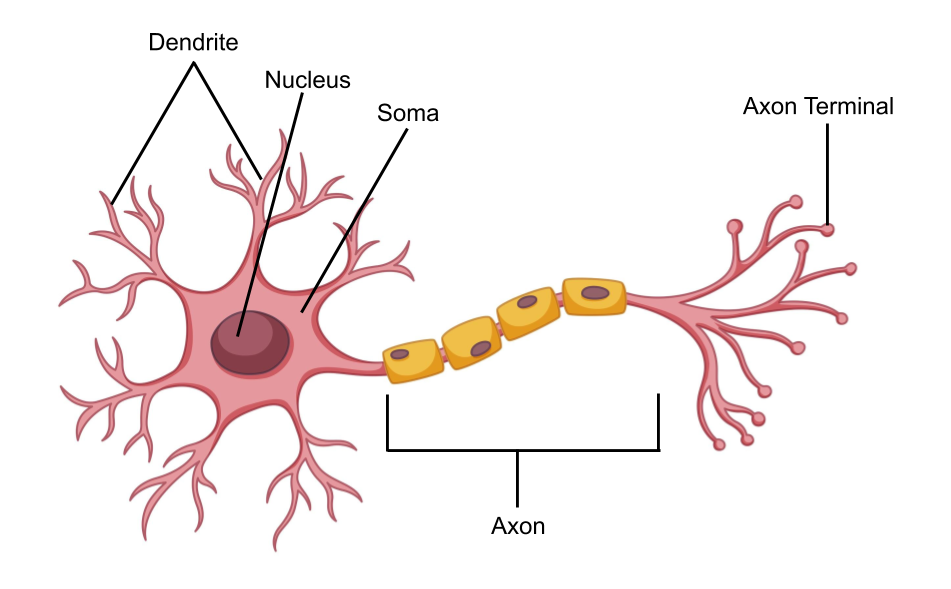
\includegraphics[scale=.25]{neuron.png} 
		\end{center} 
		\caption{\textit{Schematic representation of a neuron \cite{42}.}} \label{neuron}
		
	\end{figure}
	
	The importance of the brain in mammals is by today extremely evident: this vital organ allows us to think,  to capture the stimuli from the environment and elaborate them, enriching our memory and  our learning. The brain is the control center of our movements and our actions, it allows us to speak, to understand other individuals and elaborate responses. Most importantly for this work, however, the brain, from its basic cellular units, can explain our behaviour and our emotions. \\

	
	The brain itself is part of the \textbf{nervous system (NS)}, and its most important cell is the \textbf{neuron}.	Neurons are one of the basic unit needed for the transmission of
	the electric signals, both within the same area and between different areas of
	the brain, allowing the NS to collect information and to react to stimuli,
	elaborating decisions based on them. \\
	The neuron is composed of a central body called \textit{soma}, of the \textit{dendrites}, cellular extensions which collect stimuli from near areas, and of the \textit{axon}, the biological cable connecting one neuron to another, in order to propagate information (Figure \ref{neuron}). 
	Another type of cells present in the NS are the \textbf{glial cells} (like astrocytes), which perform functions of protection, sustainment and nutrition for the neurons. Although glial cells are not the main focus of this work, their contribution to the NS should not be neglected, as it has been shown to be relevant in many important processes \cite{1}. %Semyanov]. \\
	
		
	
	Neurons are \textbf{excitable} and \textbf{conductive} cells, i.e. they can generate an electrical impulse and transmit it to other neurons, forming neuronal microcircuits, often associated with a specific area and/or task of the brain. \\
	Inside every neuron, in the cytoplasm, there is a coexistence of different ionic species (mostly $Na^+, Cl^-, K^+, Ca^{2+}$) which, in equilibrium conditions, assume a certain concentration, concurring to determine a difference between the electric potential assumed inside and outside the cell: we call this quantity the \textbf{membrane potential} of the cell (indeed it is the potential drop formed across the cell's membrane).  In reaction to an external stimulus, the ionic concentrations change rapidly their values, provoking a heavy change in the membrane potential. As a consequence, the excitation of a neuron happens, as well as the formation of an \textbf{action potential}, which will propagate to other neurons along the axon (Figure \ref{membrane}). 
\begin{figure}[H]
	\begin{minipage}{\linewidth}
		\centering
		\begin{minipage}{0.45\linewidth}
			\begin{figure}[H]
				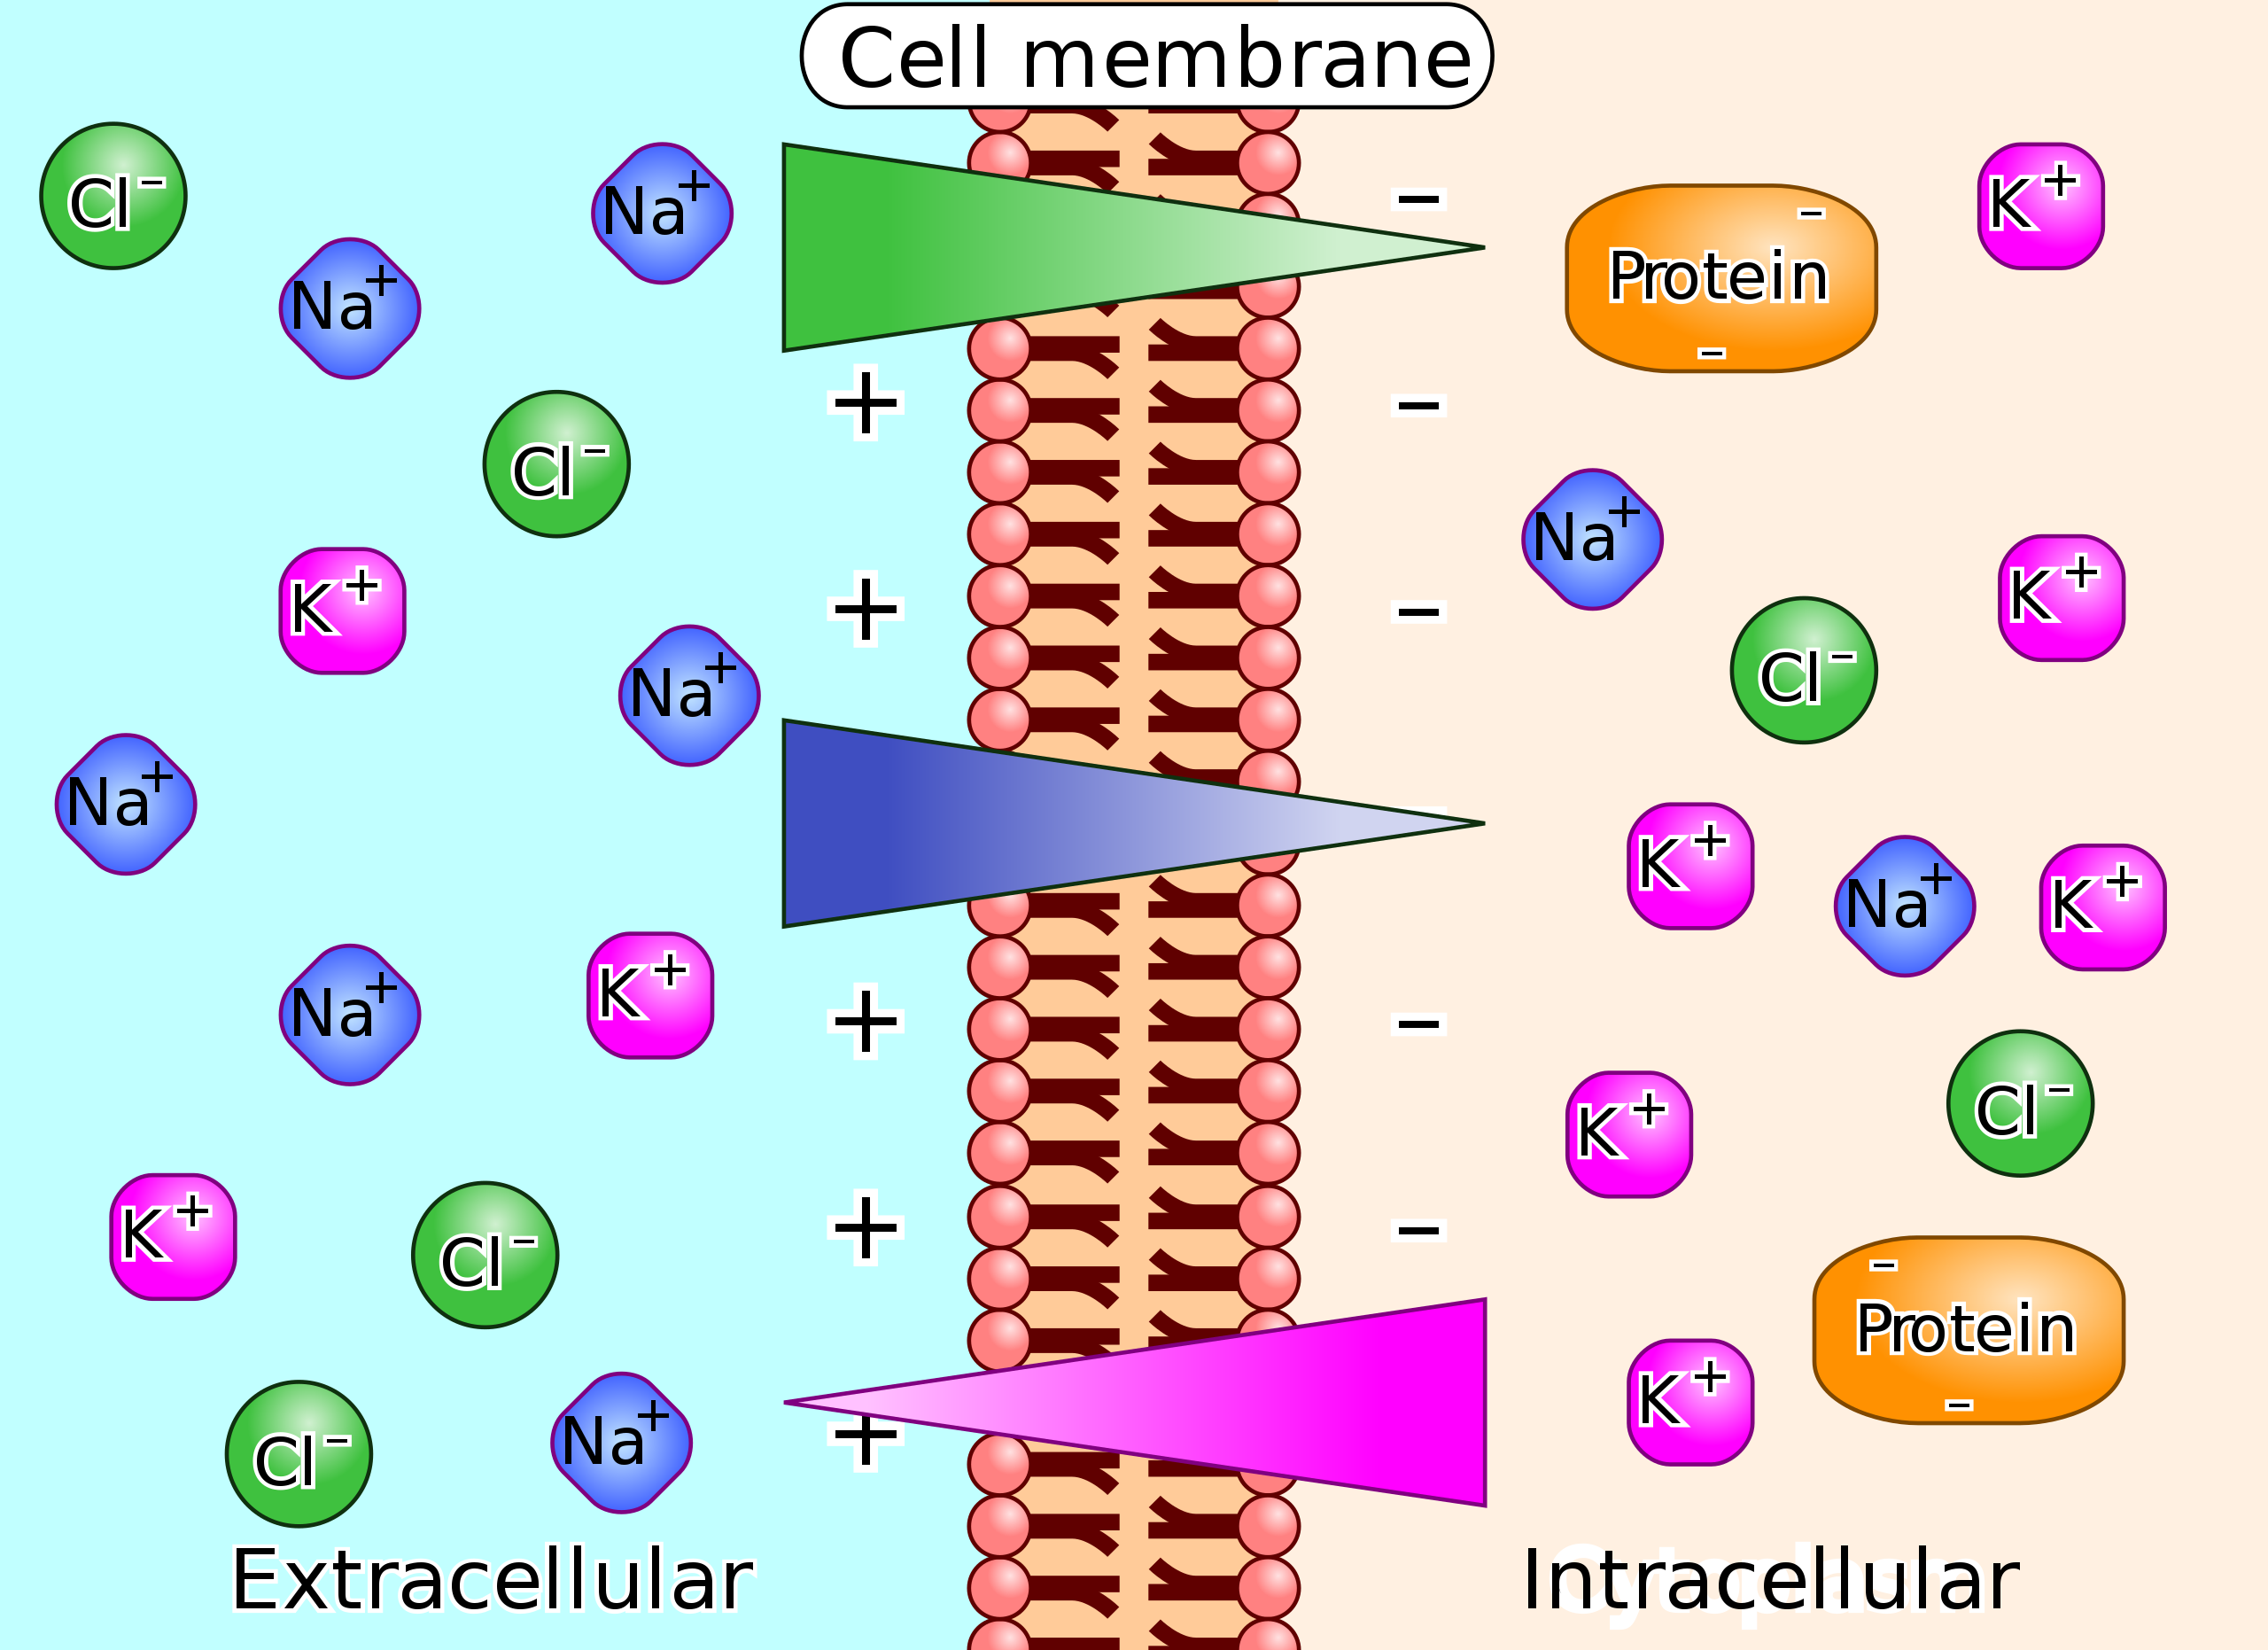
\includegraphics[width=\linewidth]{AP1.png}
				
			\end{figure}
		\end{minipage}
		\hspace{0.05\linewidth}
		\begin{minipage}{0.45\linewidth}
			\begin{figure}[H]
				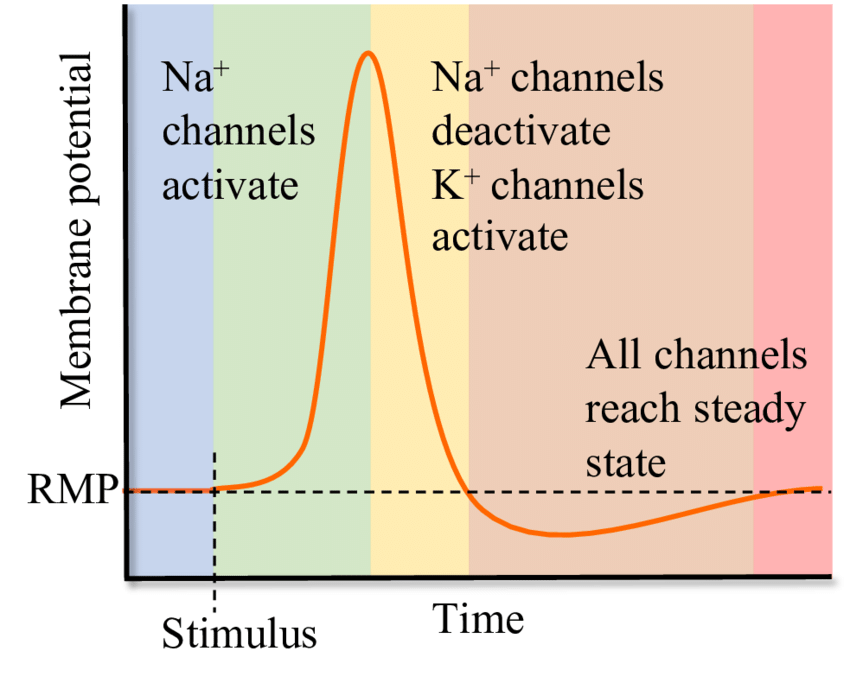
\includegraphics[width=\linewidth]{AP2.png}
				
			\end{figure}
		\end{minipage}
		
	\end{minipage}
\caption{\textit{Left: schematic representation of ionic species inside and outside the cellular membrane. Such species are allowed to pass through the membrane only in specific circumstances through adhibited ionic gates. \\
Right: example of action potential formation in reaction to a stimulus. \cite{43}}}\label{membrane}
\end{figure}

At the end of the axon, the link between a neuron and its neighbour, and the relative passage of the electrical impulse, occurs thanks to a chemical \textbf{synapse} (Figure \ref{synapse}), a particular structure located in the terminal of the axon. Here, special molecules called \textit{neurotransmitters} are syntethized, and the arrival of an action potential allows such molecules to travel towards the \textit{intersynaptic space}, where they can bind to receptors located in the post-synaptic cell. The response of the post-synaptic cell, then, can be either excitatory or inhibitory, based on whether the impulse is preserved in the circuit or supressed.\\
The synapses (and thus their corresponding neuron) can be classified in four main groups, depending on the type of neurotransmitter which they release:  glutamatergic, GABAergic, cholinergic,  adrenergic. The most relevant for this work will be the one of GABAergic synapses, consisting of inhibitory neurotransmitters which reduce the excitability of the neurons.\\

In neurobiology, the conditions under which a neuron can be considered \textbf{active} are not unique and matter of debate. When discussing \textbf{neural activity}, the literature usually means either the already discussed electrical activity, or the \textbf{calcium activity}. The intracellular dynamic of this particular element, in ionic form of $Ca^{2+}$, is known to be essential for the main cellular processes, and is strictly related to the formation of an action potential and subsequent propagation of the electrical impulse.\\
 Indeed, we can usually observe  \textit{strong instabilities} in the intracellular calcium concentration (Figure \ref{oscillations}), which often show fast oscillations and changes, through the formation of sudden peaks: we will define the neuron as \textit{active} in correspondence to these peaks.
 
 
 \begin{figure}[H]
 	\begin{center}
 		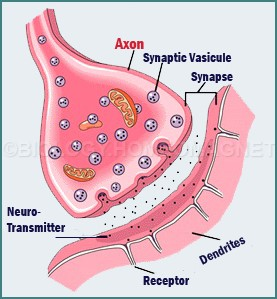
\includegraphics[scale=0.2]{synapse.jpg} 
 	\end{center} 
 	\caption{\textit{Schematic representation of a chemical synapse \cite{44}.}}\label{synapse}
 	
 \end{figure}

\begin{figure}[H]
	\begin{center}
		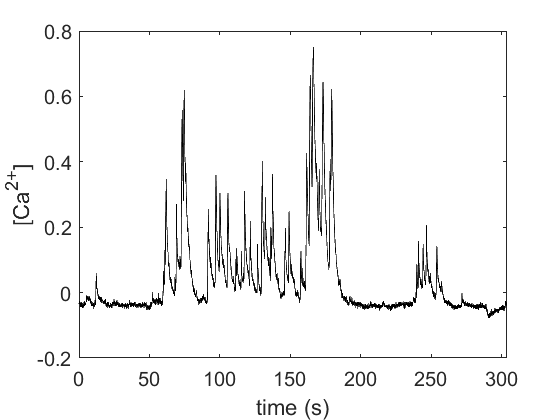
\includegraphics[scale=.50]{Ca_conc.png} 
	\end{center} 
	\caption{\textit{Example of $Ca^{2+}$ concentration recorded in a neuron, as a function of time.}} \label{oscillations}
	
\end{figure}
	
	Having defined the meaning of neural activity, we can ask ourselves whether this activity may be related to aspects like behaviour, emotion, body language, mood: in other words, to investigate whether there is a connection between the activation of some specific neurons, and what animals do.\\
	This topic has fascinated neuroscientists for decades, and from what it has been discovered so far, it seems evident that \textbf{different brain circuits are responsible for different behaviours} (although these distinctions may not always be that marked, unique and easy to detect).

	
	The neurobiology experiments on which this work relies on refer mainly to some particular areas of the brain, which previous studies found to be strictly connected to emotional and behavioral processes \cite{2}: %[Etkin et al. 2011]:
	\begin{itemize}
		
		\item \textbf{Medial prefrontal cortex (mPFC)}:  part of the frontal cortex, the area of the brain located in the frontal lobe. This area is implicated in cognition processes, including socio cognitive abilities,  with strong connections with decision making \cite{3} % [Carlen 2017]
		
		\item \textbf{Anterior Cingulate Cortex (ACC)}: part of the cingulate cortex and situated in proximity of the mPFC,  with which  ACC shares a lot of functionalities. Indeed, experimental evidence of the connection between this area of the brain and emotions have been found \cite{4}. %[Zheng 2020]
		 This area seems also to be implicated in social aspects like morality or empathy \cite{5}, % [Carillo 2019],
		  as reaction to interactions with another individual
		
		\item \textbf{Amygdala}: nuclear complex located in the medial part of the temporal lobe. It is responsible for the elaboration of the emotions, it collects stimuli from the thalamus and elaborate responses: in other words, it plays the role of emotional thermometer of the body and the decision maker for adequate responses \cite{6} %[Banks]
	\end{itemize}


	
	\begin{figure}[H]
		\begin{center}
			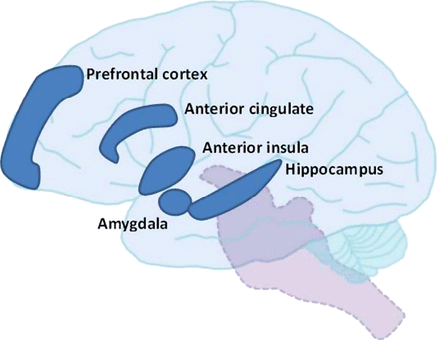
\includegraphics[scale=.75]{brain.png} 
		\end{center} 
		\caption{\textit{Main areas of the brain involved in behaviour and emotion recognition \cite{45}.}}
		
	\end{figure}

\newpage

\section{In vivo studies on mice}

According to the \textit{Foundation of Biomedical Research (FMR)}, approximately $95\% $ of all lab animals are mice or rats, as in the case of the current work. Although very often the final goal of the research is an application useful for humans, the reasons why mice are the first choice for experiments are numerous. First of all, mice are mammals quite similar to humans when it concerns genetics, at the point that scientists have been able to reproduce genes in mice similar to the ones implied in human diseases ("\textit{transgenic mice}" \cite{7}); %[Harari,Abramovich 2014]);
 rodents, indeed, are also easy to manipulate from a genetic point of view. Another reason is definitely the fact that mice are small, easy to control, quite cheap to buy and usually docile. Finally, being the most used animal in research, the largest information and literature which can be found is about them, their anatomy, their typical behaviours, and by today large populations of rodents have been created and used exclusively for experimental purposes, being almost all identical and therefore setting a uniform standard for study and validation of results. \\
In the experiments, through a  \textbf{behavioral task}, one or more mice are put in a particular situation designed to study their reactions, such as a shown behaviour or movement, and, in this context, the goal is to find a relationship with their correspondent neural activity. Therefore, the overall experiment consists in the following steps:
\begin{enumerate}
	\item Preparation of the arena and equipment for the task 
	\item Preparation of the mice for the experiment, both in terms of behavioral conditioning, and for neural activity measurements
	\item Performance of the test with simultaneous recordings of  aspects of interest such as behaviour or neuronal activity
	\item Pre-processing and analysis of the collected data
\end{enumerate}

\begin{figure}
	\begin{center}
		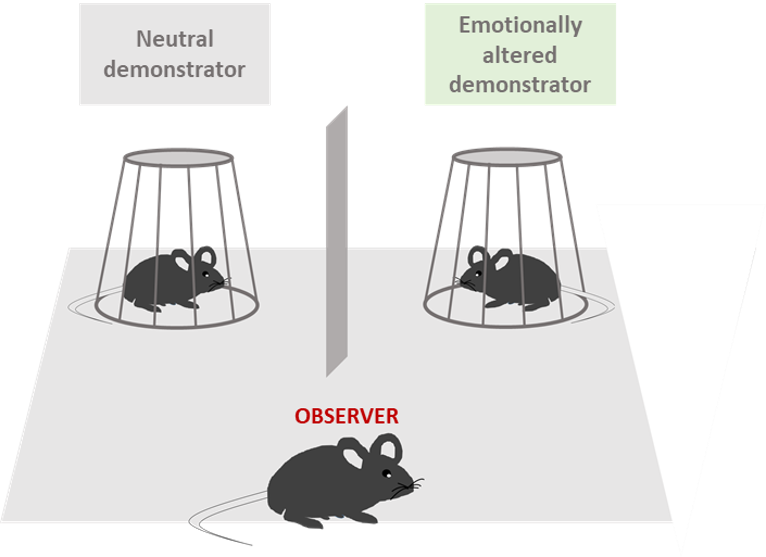
\includegraphics[scale=.70]{mice_task.png} 
	\end{center} 
	\caption{\textit{Basic setting of the emotion discrimination task: one mouse (the \textit{observer}) is free to move in the arena, while the others two (the \textit{demonstrators}) remain inside a cage. One of the demonstrators has a neutral affective state, the other an altered affective state.}} \label{emotion discrimination}
	
\end{figure}
In this work, the behavioural task under investigation in chapter 3 is a particular realization of the \textbf{emotion discrimination task}, schematized in Figure \ref{emotion discrimination}. The first step of these types of tasks, performed in this way several times in the past, sees the presence of three mice: one, called the \textbf{observer}, is a mouse free to move in an arena, while the others two, called the \textbf{demonstrators}, remain in a cage. In the phase preceding the test, the \textit{habituation phase}, one of the two demonstrators is \textit{emotionally altered}: namely, it is subjected to specific conditions and procedures which provoke an alteration of its affective state. This alteration could be either negative (usually stress condition following a 15-minutes period of restrain) or positive (usually relief condition, consisting in water \textit{ad libitum} following water deprivation). The other demonstrator and the observer are instead in a \textit{neutral} state.\\

Previous works on this setup \cite{8} %[Scheggia-Managò]
 were performed using both positively and negatively affected demonstrators. The cellular target consisted in a specific subpopulation of neurons, which is thought to be involved in processes like \textit{affective state discrimination}: the \textbf{somatostatin (SOM+)} interneurons in the medial prefrontal cortex.\\
These neurons, expressing the somatostatin neurotransmitter, form a small
subgroup of inhibitory neurons, distinct from others like pyramidal neurons or parvalbumin interneurons (PV+). Pyramidal neurons, called in this way because of the shape of their soma, are the most common units of \textit{excitatory} type present in the PFC, and are mainly involved in \textit{cognition} processes such as object recognition. On the other side, also PV+ neurons, expressing the \textit{parvalbumin} neurotransmitter,  are  very common in the PFC. However, only SOM+ neurons seem to be directly implicated in the affective state discrimination of a conspecific mouse. The \textbf{CRE system} \cite{8} ensures that the targeted neurons are SOM+: the mice have been genetically modified in such a way that only SOM+ neurons present the Cre-recombinase genetic sequence. Then, the injection of the adenovirus DIO-GCaMP makes it bind only to neurons expressing the Cre sequence. These neurons will present  distinctive features (such as fluorescence) which will allow to recognize them and collect data, using the techniques described in the following. \\
The data analysis on the task showed some remarkable results:

 \begin{itemize}
 	
 	\item The time spent by the observer near the altered demonstrator was significantly higher than the time spent near the neutral demonstrator. A similar consideration holds for the duration of the moments when reciprocal sniffing between two close mice happened (Figure \ref{Scheggia})
 	
 	\item This  discrimination appears to be stronger in the first period of the test
 	
 	\item The discrimination is directly connected to the presence of a mouse in an altered state (both negative and positive), since from the repetition of the task using only two neutral demonstrators no significant differences emerged
 	
 	\item By repeating the task eliminating one sense at a time, it has been shown that the main sense responsible for the discrimination is olfaction. However, in order to achieve the same results of the test, a combination of both olfactory and visual cues is needed
 	
 	
 	\item The neural activity of the observer (both in terms of electrical impulse and  calcium peaks) showed stronger values during the interactions with the altered mouse, rather than the neutral one
 	
 	\item If optogenetic inhibition of SOM+ cells \cite{41} is
 	performed on the observer before the test, the discrimination disappears, namely no relevant differences between time spent and sniffing behaviour have been observed in relation to the altered demonstrator rather than the neutral one
 	
 	
 	\item All the previous considerations do not apply to other neuronal categories like pyramidal or parvalbumin interneurons
 	 
 \end{itemize}
 
 Overall, these results seem to show a \textbf{key role of the somatostatin interneurons in affective state discrimination}.

	\begin{figure}
	\begin{center}
		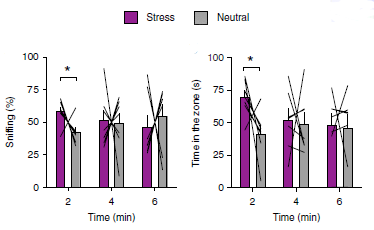
\includegraphics[scale=0.68]{scheggia.png} 
	\end{center} 
	\caption{\textit{Recording of sniffing times (left) and proximity times (right) between observer mouse and stressed demonstrator (purple) and observer mouse and neutral demonstrator (grey).}} \label{Scheggia}
	
\end{figure}


Other examples of emotion discrimination in mice related to SOM+ interneurons can be found in \cite{9}, %[Mariotti et al 2018],
 with a focus on their effect on cortical astrocytes: the main result shown in the study consist in a \textbf{crucial role of somatostatin} in the stimulation of responses by astrocytes.
As a first result, it has been shown that the stimulation of SOM+ interneurons (via 10-pulses light stimulation of calcium indicators), increases the $Ca^{2+}$ response from astrocytes. Also in this case, a comparison with PV+ interneurons show the \textit{critical sensitivity of astrocytes only to SOM+ interneurons, but not PV+}. Overall, this study reveals that a sustained activity in the SOM+ interneuron circuits is complemented by
a sustained activity in the astrocytic network, thus confirming the importance of astrocytes and their link to inhibitory neuronal circuits. 
\\

Somatostatin is not the sole neuropeptide that has been shown to be linked to emotion discrimination. For example, in \cite{10}, % [Ferretti-Maltese 2018], 
the in vivo task on mice targets the \textbf{oxytocin (OXT)} neurotransmitter, studying its release in the central amygdala. The behavioral task of this study has a similar structure to \cite{8}, in which neutral and altered demonstrators were contraposed to an observer mouse. Also this case shows evidence of  discrimination caused by the altered mouse (for example, through an increased sniffing activity), as well as the importance of olfactory clues in the process of such discrimination.\\
A reduction of  OXT level in the central amygdala resulted in the \textit{abolishment} of emotion discrimination, while a new increase of such level resulted in the rescue of the former conditions, thus remarking the central role of the OXT neuropeptide in the emotion discrimination.
\\

When targeting a specific neuronal subpopulation, the hope is to always find  more evidence on its connection with  properly shown tendencies, emotions or behaviors that are common to known diseases. In the case of the emotion discrimination task targeting SOM+ interneurons in the mPFC, for example, the observed effects in the abolition of discrimination, following photoinhibition of such neurons, could be similar to the ones observed in neurodevelopmental disorders such as autism spectrum disorders (ASDs) or schizophrenia. Therefore, this approach aims to investigate the causes of a specific issue at a basic and detailed level such the one of single neuron precision, with the ultimate goal of acting on such level to perform a change on the macroscopic effects.\\
In order to do so, the paradigm of the task has to be defined in a way that it allows a collection of unbiased results, but an adequate way to perform an imaging of the neuronal activity of interest is necessary as well (and described in the following sections). As a final step, a proper data analysis on those results has to be performed (in the present case, using the methods introduced in Chapter 2).


\section{Calcium imaging through Inscopix} \label{section 1.3}



\begin{figure}[H]
	\begin{center}
		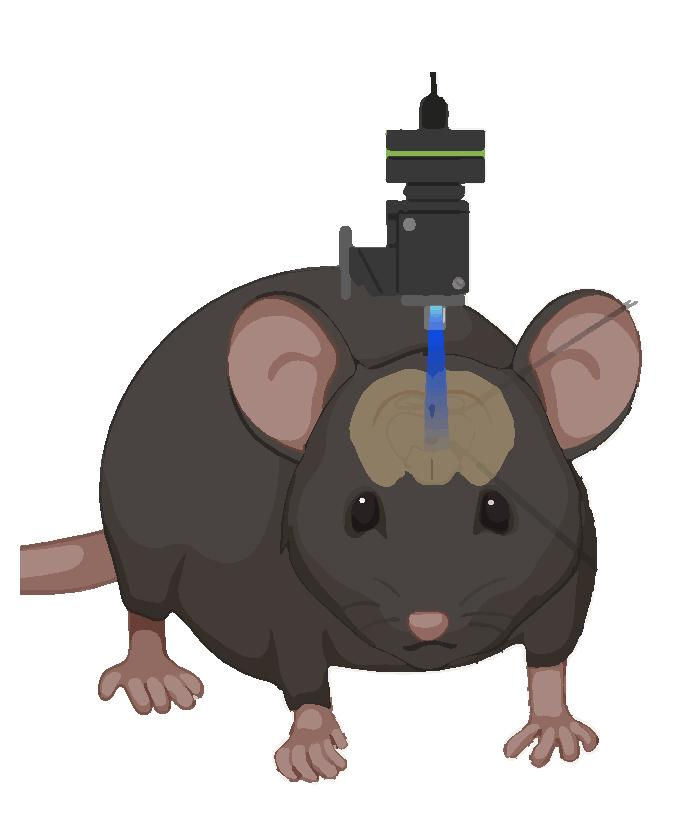
\includegraphics[scale=.35]{Inscopix.jpg} 
	\end{center} 
	\caption{\textit{The Inscopix miniscope.}}
	
\end{figure}


In this section, a powerful tool for single neuron calcium imaging will be presented: \textbf{microendoscopic calcium imaging}. The Inscopix company \cite{11} %[https://www.inscopix.com/]
 provides tools and software to extract calcium tracks as one photon measurements from in vivo experiments on mice.\\
To measure the intracellular $Ca^{2+}$ concentration in a single neuron of a mouse during a behavioral task, the first step is the performance of a surgery on the mouse to implant a miniscope in the \textit{region of interest (ROI)} of the brain to be investigated. On the same mouse, \textbf{genetically encoded calcium indicators (GECI)}, such as the \textbf{GCaMP} protein, are adopted. These types of proteins, when bound to $Ca^{2+}$, emit a fluorescent light, which intensity will be captured by the miniscope. At the end of the test, the miniscope will be able to give back a video of the ROI, in which the evolution of the fluorescence through time can be appreciated  in the neurons, as shown in Figure \ref{inscopix}. In this way, it is possible to obtain a representation of the intracellular calcium oscillations behaviour during the whole task. This information can be combined with behavioural or positional data of the mice in the arena, making it possible to start a data analysis and look for correlations between behaviour and neural activity.\\
In order to have the data ready to be analyzed, the Inscopix software manages also the pre-processing part, which goes through the following steps:

\begin{figure}[H]
	\begin{center}
		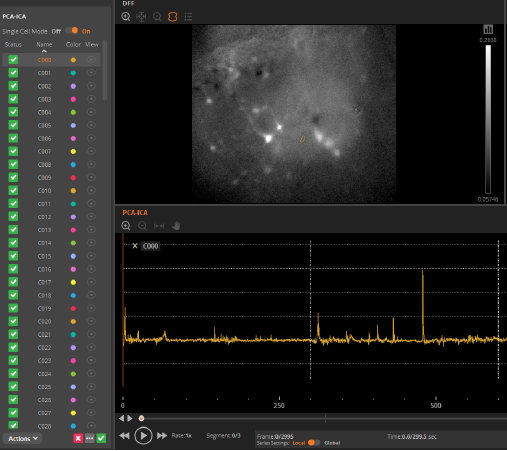
\includegraphics[scale=.80]{Inscopix2.png} 
	\end{center} 
	\caption{\textit{Example of pre-processing work through the Inscopix software. We can appreciate: the list of detected neurons (left), a segment of the video in the ROI (top-right) and an example of the calcium track recorded in a single neuron through time (bottom-right).}}
	\label{inscopix}
\end{figure}

\begin{enumerate}
	
	\item If needed, more videos recorded from the task can be combined, in order to obtain a single final video of the ROI through time
	
	\item \textbf{Spatial and temporal downsampling} are performed, selecting the appropriate scale factors of space and time which allow to capture all the important information
	
	\item \textbf{Spatial filtering} of the image: it removes low and high frequencies with a bandpass filtering. The filter has the form
	
	$$ M_f^{band} = GB(M_f,\sigma_{high}) - GB(M_f,\sigma_{low})$$
	
	Where $M_f$  represents the frame $f$ of movie $M$, $GB$ is the \textit{Gaussian Blur} function, and the standard deviations $ \sigma_i = \frac{2 ln(2)}{2 \pi \lambda_i}$ are computed from the cut-off values $ \lambda_{high}$ and $ \lambda_{low}$
	
	\item \textbf{Motion correction}: it accounts for the motions between different frames of the videos, applying a correction to let every pixel staying at the same place along the different frames of the movie
	
	\item \textbf{Pixel normalization}: each pixel of a frame represents a different luminosity, caused by the fluorescence obtained from the reaction with the GCaMP. After the preprocessing, the value of the fluorescence (which estimates the calcium concentration) is expressed as 
	$$\frac{\Delta F }{F} = \frac{F(x,y,t) - F_b}{F_b}$$
	where $F(x,y,t)$ represents the measured fluorescence at the point $(x,y)$ at time $t$, while $F_b$ is a baseline fluorescence value (usually the mean value of the movie, in some cases the minimum). After this step, the returned value for every pixel is an adimensional relative value of fluorescence
	
	\item The \textbf{PCA-ICA algorithm} attempts to recognize the neurons of the ROI in the movie. Based on given information such as average cell's diameter, a principal component analysis (PCA) is performed, followed by an independent component analysis (ICA), until convergence. In particular, the frames of the movie, represented as matrices, are rasterized into 1D vectors and they are normalized on mean and standard deviation. At this point, a principal component analysis is performed, in order to reduce dimensionality. Every frame is then approximated by a weighted sum of the principal trace components. Finally, an ICA algorithm is launched. At the end of this process, every neuron will be identified, labeled, and gifted with a calcium activity value (which is actually  $\frac{\Delta F }{F}$) for every time instant of the movie. 
	
	\item \textbf{Final adjustements}: appropriate algorithms or manual fixing are performed to take into account some imperfections, such as mistakes in neuron identification, inaccuracies due to overlapping neurons, excessive noise in the calcium traces for a neuron (discarding the corresponding cell from the analysis)
	
	\item \textbf{Data import}: finally, data are imported in a csv file and are ready to be analyzed (in this work, using the software \textsc{Matlab})
	
\end{enumerate} 


At the end of all these steps, the final data available consist of a list of every neuron detected, and the corresponding recorded value of $\frac{\Delta F }{F}$ associated  with each neuron for each time instant. The preprocessing step is now over, and the calcium traces of every neuron in the ROI are available for the data analysis process.	


\newpage
\section{Calcium imaging through Fiberphotometry} \label{section 1.4}

\begin{figure}[H]
	\begin{center}
		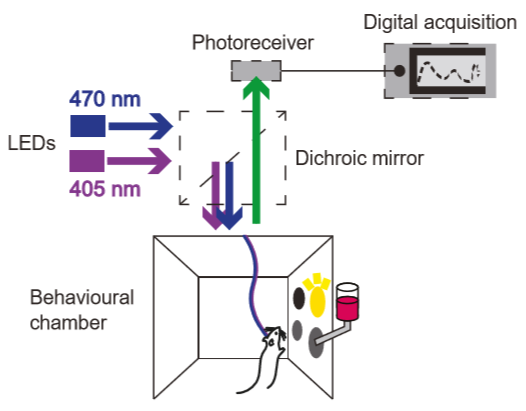
\includegraphics[scale=.55]{fiberphotometry.png} 
	\end{center} 
	\caption{\textit{Fiberphotometry experimental setup}}
	\label{fiberphotometry}
\end{figure}

In the previous section, it has been shown a calcium imaging technique based on single neuron traces, measured with single photon miniscopes. In this section, another common technique for calcium imaging is under investigation: \textbf{Fiberphotometry} (Figure \ref{fiberphotometry}). \\
Although the main goal of this technique is the same as the Inscopix imaging one, technical equipment, methodology and results present substantial differences.\\
Relying on genetically encoded calcium indicators such as GCaMP, with fiberphotometry the fluorescence signal is recorded through \textit{optic fibers}, typically of length $300-400$ $ \mu m$. An excitation of GCaMP is performed using a blu LED light at the appropriate wavelength ($470$ $ nm$), which is transmitted through the optical cannula implanted in the mouse, while an emission green light ($525$ $ nm$) is relayed to a photoreceiver. Often, a second excitation light (violet, $405$ $nm$), is used as well, to take into account autofluorescence and produce an isosbestic (calcium-independent) control signal \cite{12}. \\% [Girven].\\
 Finally, a software manages the output signal in order to perform filtering and return a collective raw signal, separating the two contributions from blu and violet lights. Such signal, unlike the miniscope neuronal imaging, can only be an \textit{aggregate} signal of the observed area. This implies that the Fiberphotometry technique produces signals at lower spatial resolution than the previously introduced technique of microendoscopic imaging. However, this technique is becoming increasingly popular because its smaller accuracy is compensated by several positive factors:

\begin{itemize}
	
	\item The overall experimental setup for Fiberphotometry results cheaper than the one for miniscope imaging 
	
	\item The procedure operated in mice are less invasive, and the subjects are more suitable to long freely behaving experiments
	
	\item The implant of the cannula is relatively easy to perform, and a good signal is collected even with fiber placements in the neighborhood of GECI-expressing populations 
	
	\item Multiple areas of the brain can be investigated at the same time 
	
	\item Fiberphotometry can be used for other fluorescent indicators, such as norepinephrine, % (Feng et al., 2019),
	 GABA, %(Marvin et al., 2019), 
	 glutamate, % (Liang et al., 2015),
	acetylcholine, % (Jing et al., 2018) 
	and dopamine \cite{12} %(Patriarchi et al., 2018)
	
	
	
\end{itemize}


\section{Synchronization of neural activities} \label{section 1.5}

\begin{figure}[H]
	\begin{minipage}{\linewidth}
		\centering
		\begin{minipage}{0.6\linewidth}
			\begin{figure}[H]
				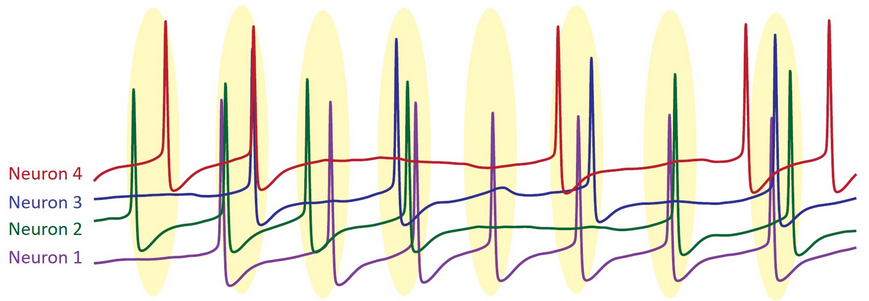
\includegraphics[width=\linewidth]{synch.png}
				
			\end{figure}
		\end{minipage}
		\hspace{0.05\linewidth}
		\begin{minipage}{0.6\linewidth}
			\begin{figure}[H]
				\includegraphics[width=\linewidth]{Intebrain.png}
				
			\end{figure}
		\end{minipage}
		
	\end{minipage}
\caption{\textit{Top: single neuron synchronization.
		Bottom: overall activity synchronization}} \label{synch}
\end{figure}

In the previous sections, the concept of \textit{neural activity} has been introduced in its different shapes. Not only it can be identified with the electrical and calcium activity, but \textit{activity} necessarily refers to a specific area: it can be the activity of a single neuron or of a group of neurons in a ROI (often, in this case, the activity is attributed to the whole animal for that specific context). In any case, the main object of interest is a \textbf{signal evolving in time}.\\
While, historically, the study of neural activity has been mostly dealing with signals of single individuals treated one by one, the focus, in the most recent years, is extending to cover as well a more complex topic: the \textbf{synchronization between different brain activities}. The definition of synchronization between signals, not unique and assuming different shapes for different needs (Chapter 2), can involve two types of correlations (Figure \ref{synch}):

\begin{itemize}
	
	\item \textbf{Intraneuronal synchronization}: the signals of  single neurons show a correlated activity.The relevance of this phenomenon is to look for correlations \textit{within} the same region of interest (ROI), namely for correlations among the neurons of the same animal in a particular area of its brain. However, the correlation could be investigated as well between different areas of the same individual
	
	\item \textbf{Interbrain synchronization}: the synchronization is studied among two different individuals. This could be done either considering neurons from the two subjects firing simultaneously, or defining the whole activity of one individual (for example through a mean of its neuronal activities) and looking for its synchronization with the whole activity of another individual
	
\end{itemize}

In the first type of synchronization,  the correlation between a subset of neurons in the same individual is a property of a \textit{neural circuit}: it has been observed that the chain of firing of neurons (both in electrophysiology and calcium imaging) often exhibits some \textbf{patterns}. This means that some neurons tend to show simultaneous peaks through time, or a similar order and timing of firing. The presence of correlated activity in a ROI has been shown to be linked with expressed behaviours \cite{13}, %[Frost et al. 2020], 
leading to the conclusion that \textbf{different behaviors can cause the synchronizations of different  subpopulations of neurons}.\\
This phenomenon could be independent by a rise of neural activity as consequence of an observed behaviour, in the sense that, in principle, it may happen that a rise in a correlated activity does not correspond to a rise in neural activity and viceversa. One of the goals of the correlation analysis is the \textbf{identification of a group of neurons encoding a specific behaviour}. The neuronal ensemble in terms of synchronization may be different from the neuronal ensemble in terms of activity peaks (even if often the intersection of the two is quite significant \cite{8}).\\
In the second type of synchronization, the \textbf{interbrain synchronization}, the correlation analysis is performed between signals of different individuals; this could be intended both for single neurons and for  overall individual activities. Therefore, this type of synchronization is studied through an \textit{interaction} between two subjects. Again, the goal is either to find an ensemble of neurons which tend to correlate to the partner ones, or to show that in specific situations the correlation between subjects increases or decreases.\\

\begin{figure}[H]
	\begin{center}
		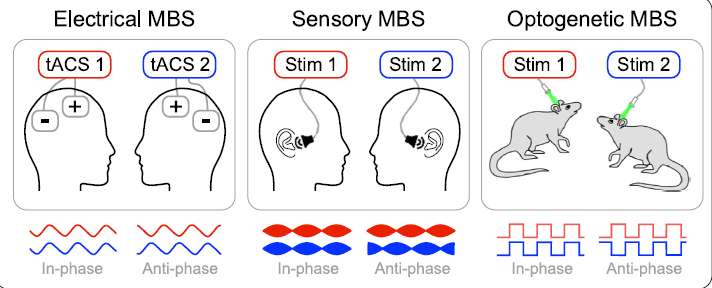
\includegraphics[scale=.70]{novembre.png} 
	\end{center} 
	\caption{\textit{Example of multi brain stimulation techniques.}} \label{mbs}
	
\end{figure}
Previous works \cite{14} % ([Wass et al. 2020])
 have been performed on humans in order to investigate the causes and effects of interbrain synchrony (often referred to as \textit{hyperscanning}). Performing an \textbf{electroencephalography (EEG)} on two interacting subjects, a strong connection has been identified between a rise in synchronization  and aspects like interpersonal coordination, cooperation and communication. In \cite{15}, %[Novembre et al. 2021], 
 this relationship is further inspected: the simultaneous presence of synchronization and behaviour is not enough to establish a \textit{causality} between the two, which, instead, can be shown only by studying the effects which the manipulation of the first causes on the second, or viceversa. This is achieved through \textbf{multi brain stimulation (MBS)} (Figure \ref{mbs}): stimulation processes (usually of non invasive type in humans, invasive on animals) are performed on the subjects, and the provoked effects measured. Therefore, a correct analysis should combine the two approaches (hyperscanning and MBS) to be able to show true causality between interbrain synchrony and behaviour.
\\

As for Interbrain analysis on mice based on microendoscopic calcium imaging, few works have been done and the topic is still largely unexplored. In one of the most significant papers, \cite{16}, % [Kingsbury et al. 2019],
 intracellular calcium has been recorded from neurons of the mPFC in two subjects interacting in an open arena.  The mean activity ($\frac{\Delta F }{F}$) has been computed for every mouse, and the correlation between the two corresponding signals has been computed as well (using mostly cross-correlation, see Chapter 2). The first result was that animals engaged in social interaction showed higher interbrain synchronization, reporting higher values of correlation during social interaction rather than solitary periods. Moreover, the abolishment of physical interaction, using a barrier, resulted as well in the inhibition of interbrain correlation, meaning that the synchronization is not due to environmental factors, but instead strictly related to the direct interaction between conspecifics (Figure \ref{kingsbury}).\\

\begin{figure}[H]
	\begin{center}
		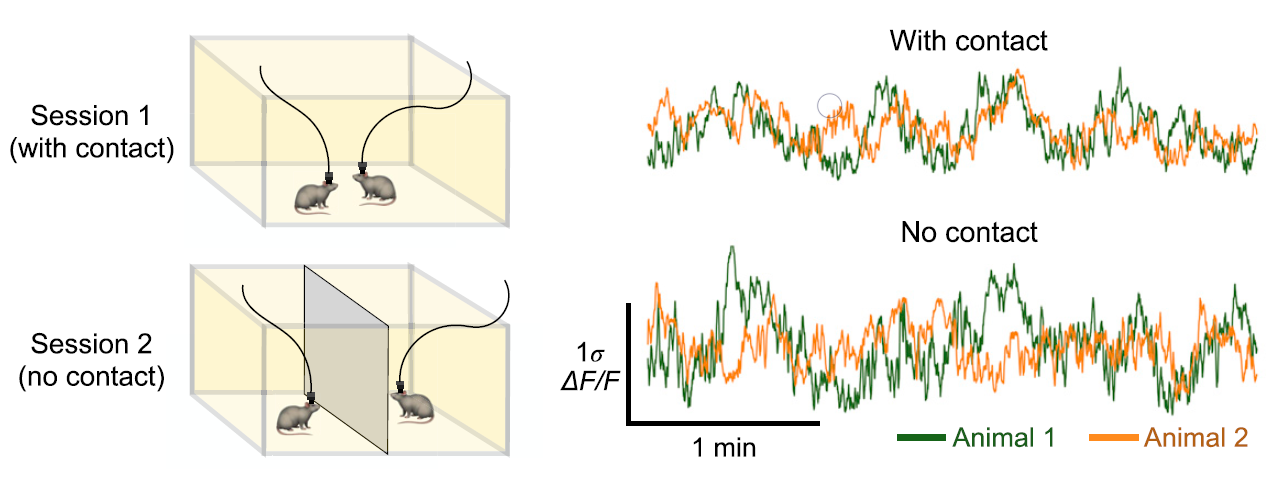
\includegraphics[scale=.45]{kingsbury.png} 
	\end{center} 
	\caption{\textit{Comparison of neuronal activities in the two mice with and without contact.}} \label{kingsbury}
	
\end{figure}


The second task performed in the experiment was the \textit{tube test}, in which the two subjects were placed facing each other in a horizontal tube, allowing the passage of only one individual. In this configuration, the mice can assume three types of behaviours: \textit{approach, push}, and \textit{retreat}; here animals showed again synchronization during the competitive encounters. In particular, a classification of neurons as behavioral cells allowed to link subgroups of neurons with the three types of behaviors depending on their activity values (Figure \ref{classification}). Interestingly, the removal of these behaviour cells resulted in a marked reduction of the correlated activity. Finally, between the two animals, it was evident that one would tend to assume the role of \textit{dominant} (prevalence of push behaviour), while the other of \textit{subordinate} (prevalence of retreat). Through generalized linear models (GLMs), it has been proposed a description of the dependence between the behaviour of one mouse and the neural activity of the other, observing that cells in subordinates responded more to the ones of the dominant than vice-versa. The consequence at synchronization level is that the dominant dictates the \textit{rhythm} for the subordinate's signal, making it able to predict the expected behaviour of one mouse based on the activity of the other.







\begin{figure}[H]
	\begin{minipage}{\linewidth}
		\centering
		\begin{minipage}{0.35\linewidth}
			\begin{figure}[H]
				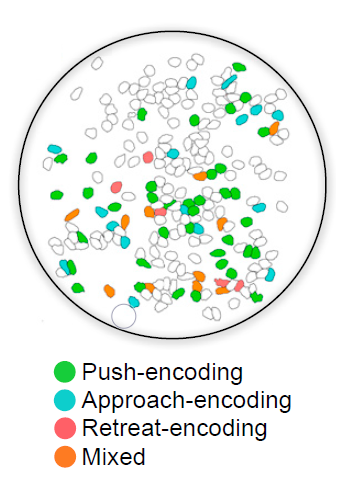
\includegraphics[width=\linewidth]{kingsbury2.png}
				
			\end{figure}
		\end{minipage}
		\hspace{0.05\linewidth}
		\begin{minipage}{0.4\linewidth}
			\begin{figure}[H]
				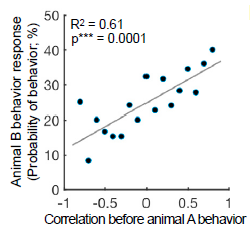
\includegraphics[width=\linewidth]{kingsbury3.png}
				
			\end{figure}
		\end{minipage}
		
	\end{minipage}
	\caption{\textit{Left: identification of behavioural neurons in the ROI.
			Right: correlation between the interbrain synchronization preceding behaviour in one animal and the response probability of the interacting partner.}} \label{classification}
\end{figure}

\newpage



\chapter{Main tools for synchronization analysis} 

In this chapter, the main tools for the analysis of synchronization between signals will be presented, with a focus on their mathematical definition and their role in the application of \textit{Intebrain synchronization}.\\
After dealing with the problem of \textit{what} synchronization actually means in this context and which measures \textit{should not} be considered, the two main tools corresponding to the two different synchronization discussed in Section \ref{section 1.5} will be presented:\textbf{ cross-correlation}, to be computed considering overall activity signals, and \textbf{peak-synchronization}, to be computed between single neurons. Each one of these tools has a specific purpose and meaning, and they will all be considered in the analysis of this work, in order to give different shapes to the concept of synchronization and to try to study it under the largest possible perspective.\\
Finally, when observing the presence of correlation between two signals, a different (although strongly connected) question may arise: "which is the \textit{relationship} of such connection?", or, in other words, "is one signal determining the behaviour of the other?". To answer such questions, a sophisticated tool will be object of study: the \textbf{Granger causality}.


\section{Understanding synchronization}

\begin{figure}[H]
	\begin{center}
		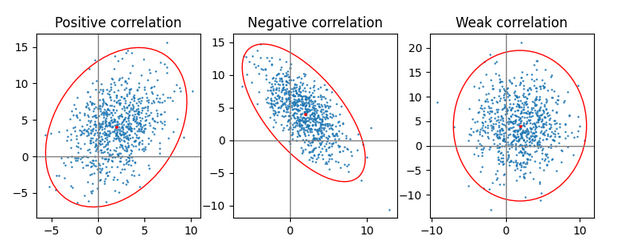
\includegraphics[scale=.75]{pearson.png} 
	\end{center} 
	\caption{\textit{Geometrical interpretation of the Pearson correlation: such coefficient gives a measure of how well the pairs obtained from the two samples distribute linearly along the diagonal of an ellipse covering the scatterplot. \cite{46}}} \label{pearson figure}
	
\end{figure}

One of the main goals of this work will be to perform a data analysis on the Interbrain synchronization of neural signals, recorded in behavioural tasks. In order to do so, first one has to clarify the meaning of the term  \textit{synchronization}.\\
In a statistical sense, the synchronization between two time series can be seen as a measure of the \textbf{correlation} between them: the more two series are correlated, the more similar and connected they will be. This leads inevitably to the fact that, when talking about synchronization, the definition can't be unique, since the similarity between two series can be assumed in different ways, depending on the particular aspect of interest. \\
However, a first hint about what to look for or not can be found in the type of signal which is under analysis. In the present case, dealing with single neuron measurements of the intracellular concentration of $Ca^{2+}$ means dealing with \textit{strongly nonlinear and unstable signals}, which exhibit sudden peaks and are often chaotic and difficult to predict.\\
For this reason, the most commonly adopted measure of correlation, namely the \textbf{Pearson correlation}, is not suited to describe such signals. Given two random samples $ \textbf{x} = \{x_i\}_{i=1}^N$ and  $ \textbf{y} = \{y_i\}_{i=1}^N$, the Pearson correlation (PC) between  $ \textbf{x}$ and  $ \textbf{y}$ is defined as

\begin{equation}
	 \rho(x,y) = \frac{Cov(x,y)}{\sigma_x \sigma_y} = \frac{\sum_{i=1}^{N}(x_i-\bar{x}) (y_i-\bar{y})} {\sum_{i=1}^{N}(x_i-\bar{x})^2 \sum_{i=1}^{N} (y_i-\bar{y})^2} \label{pearson}
\end{equation}


where:
\begin{itemize}
	\item $ \bar{x} = \frac{1}{N}\sum_{i=1}^{N}x_i$ is the sample mean
	
	\item $Cov(x,y) = \frac{1}{N}\sum_{i=1}^{N}(x_i-\bar{x}) (y_i-\bar{y})$ is the sample covariance
	
	\item $\sigma_x = \sqrt{\frac{1}{N}\sum_{i=1}^{N}(x_i-\bar{x})^2}$ is the sample standard deviation
\end{itemize}

The PC measures the \textit{linear correlation} between two quantities, as represented in Figure \ref{pearson figure}. This implies that this type of correlation should be used to inspect a linear relationship between two variables, which have a distribution close to the Gaussian one, and a uniform variance (i.e. reduced presence of outliers) \cite{17}. %[Applied multivariate statistics book by Johnson].
 Unfortunately, with the type of data incoming from the neural recordings, all these hypoteses fail, and it follows that other correlation measures should be inspected instead.


\section{Cross-correlation} \label{cc_section}

When investigating the similarity between two time-dependent signals, the first tool to be considered is the \textbf{cross-correlation}.\\
Formally, given two functions $ f = f(t)$ and $ g = g(t)$, we define the cross-correlation between them as

\begin{equation}
[f(t) \star g(t)] (\tau) = \int_{-\infty}^{+\infty} f(\tau)g(t+\tau) dt \label{cc_def}
\end{equation}


Given that the \textbf{convolution} between such functions is defined as 
\begin{equation}
[f(t) * g (t)](t) = \int_{-\infty}^{+\infty} f(t) g (t-\tau) d\tau
\end{equation}

it follows that
\begin{equation}
[f(t) \star g(t)](t) = [f(-t) * g (t)](t) 
\end{equation}

This means that the cross-correlation coincides with a convolution in which one function is considered backward in time. Moreover, in the common form of cross-correlation, as shown in (\ref{cc_def}), the resulting quantity is not expressed as a function of the time variable $t$, but as a function of $\tau$, i.e. the \textit{lag} or \textit{delay} between the signals. The interpretation is straightforward: when, for a given value of the delay $\tau$, simultaneous peaks of the two signals are both present, the contribution of their product in the integral will be more relevant for the computed value of cross-correlation correspondent to  that specific lag.\\
As a consequence of this, once computing the cross-correlation between two time-dependent functions, one can identify its maximum value and retrieve the corresponding value of the lag $\tau$, from which it is possible to obtain an estimation of the delay between the two functions. To summarize, a cross-correlation analysis allows to:
\begin{enumerate}
	\item Compute the cross-correlation between the two signals as a function of the lag value  $\tau$
	
	\item Estimate the real delay between such signals, observing when the peak of cross-correlation occurs
\end{enumerate}

When the cross-correlation is computed between the same function, it takes the name of \textbf{autocorrelation}. Confronting two identical signals, there will always be a peak of correlation (equal to $1$ using \textit{normalized} cross-correlation) corresponding to the lag $\tau = 0$. Moreover, the shape of the cross-correlation will be always symmetrical (see Figure \ref{autocorr}).

\begin{figure}[H]
	\begin{center}
		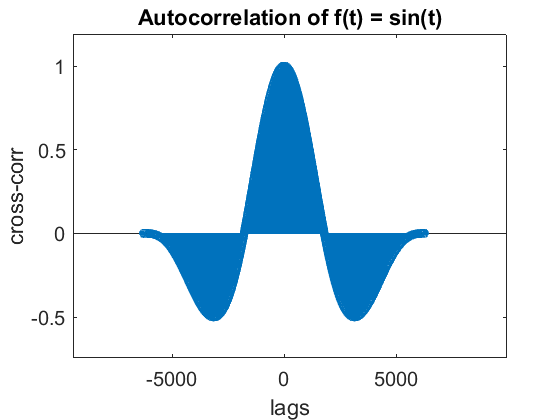
\includegraphics[scale=.75]{autocorr.png} 
	\end{center} 
	\caption{\textit{Aurocorrelation of the function $ f(t) = \sin(t) $.}} \label{autocorr}
	
\end{figure}


While the autocorrelation represents an ideal case, when dealing with two different functions $f(t)$ and $g(t)$, the significance of their cross-correlation will be given by the amount of shared properties to the case of autocorrelation; however, depending on the current application, it can be reasonable to expect a peak value in correspondence to a nonzero value of the lag, as a representation of an actual physical delay.
\\

Given two time series $ \textbf{x} = \{x_i\}_{i=1}^N$ and  $\textbf{y} = \{y_i\}_{i=1}^N$, the discrete approximation of (\ref{cc_def}) reads:


\begin{equation}
	[\textbf{x} \star \textbf{y}] (m) =  \sum_{n=1}^{N-1} x_n y_{n+m} \hspace{2cm} m_{min} < m < m_{max}
\end{equation}  

where $m$ is the approximate lag value, chosen in an appropriate interval.



\section{Peak-synchronization} \label{section 2.3}

Cross-correlation is a general and widely used tool to quantify the similarity between two signals evolving in time. With the following concept of \textbf{peak-synchronization}, the focus of the analysis is restricted to the characteristic type of signal of this work: recording of intracellular calcium activity.\\
As shown in Chapter 1, a typical recording of the activity of a single neuron is characterized by the presence of rapid and intense \textit{peaks}, which define the neuron as \textit{active}. It follows that a way to intend synchronization between neurons could be related to the presence of \textit{close} or \textit{simultaneous} peaks observed at the same time. In other words, two signals (hence, neurons) are synchronized, under the peak-synchronization point of view, if a \textit{pattern} of simultaneous firing occurs. 
\\

In order to quantify the peak-synchronization between two signals, the following steps have to be faced:

\begin{figure}[H]
	\begin{center}
		\hspace*{-0.7 cm}
		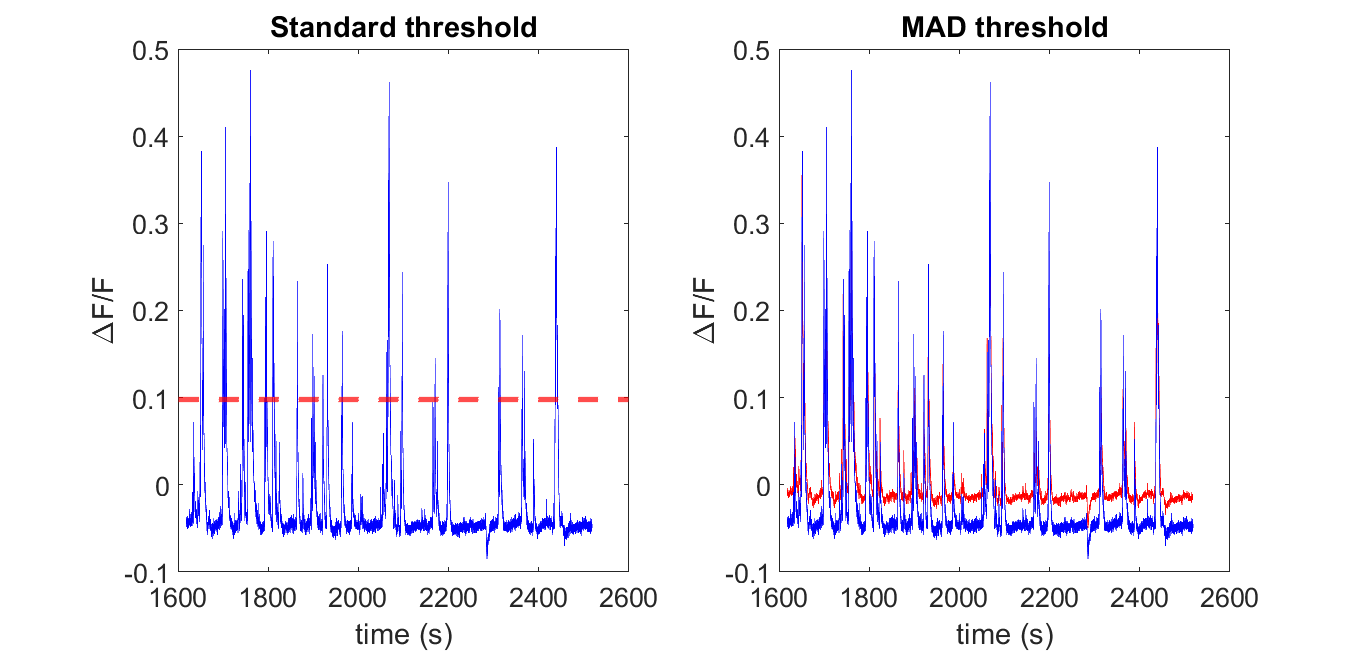
\includegraphics[scale=.45]{thresholds.png} 
	\end{center} 
	\caption{\textit{Example of a calcium signal (blue). The red curves are the thresholds built from the two algorithms: standard threshold (left panel) and MAD threshold (right panel).}} \label{threshold}
	
\end{figure}

\begin{enumerate}
	
	\item Identify when a neuron is \textit{active}, i.e. when we are in presence of a peak
	
	\item Choose an appropriate time interval in which two neurons firing simultaneously can be considered as synchronized
	
	\item Quantify the correlation between the two neurons
	
\end{enumerate}



The way to solve all of these three steps is not unique, but it is strictly depending on the current biological application under study and by the choice of appropriate algorithms for the activity detection and  synchronization quantification. In this work, the following considerations and choices have been made:




\begin{enumerate}
	
	\item  Given a discrete time series, several algorithms are available, or could be designed to detect, when a peak is occurring. A straightforward idea is to establish a threshold for the activity, in such a way that all the points above the threshold are active and all the ones below non active. Therefore, the output of such algorithm is of binary type ($1$ for activity, $0$ for non-activity).\\
	A naive way to define the threshold could be to consider a horizontal line, for example given by the equation $ y = \mu + 2\sigma $,	where $\mu$ and $\sigma$ are the mean and the standard deviation of the signal. In this way, all the values higher than $y$ will be considered active and vice versa. This approach is good enough when dealing with "well-behaving" signals, presenting a baseline low activity alternated by huge peaks, however it seems to fail when dealing with more complex and noisy signals.\\
	\begin{algorithm}
		\caption{Standard threshold algorithm}\label{tresh}
		\begin{algorithmic}[1]
			
			
			\State Consider a horizontal threshold given by $ y = \mu + 2\sigma $
			
			\State Confront every point of the signal with each corresponding point of the threshold
			
			\State Every point above the threshold is labeled as $1$, all the points below as $0$
		\end{algorithmic}
	\end{algorithm}
	
	
	For this reason, a different algorithm can be considered as well \cite{11}: the \textbf{MAD threshold} algorithm. The threshold established by this algorithm is not constant, but it "follows" the signal, in order to better capture its dynamics.\\

	
	
	\begin{algorithm}
		\caption{MAD threshold algorithm}\label{mad}
		\begin{algorithmic}[1]
			
			
			\State Start from a baseline threshold given by $ MAD = median(X_i - median(X))$, being $X$ the available dataset and $X_i$ a specific instance of it
			
			\State Identify the points where the slope changes from positive to negative (PN) and from negative to positive (NP)
			
			
			\State At every PN point, the threshold value is the MAD value plus the previous NP point's value
			
			\State The overall threshold is obtained from linear interpolation of the threshold points
			
			\State Every point above the threshold is labeled as $1$, all the points below as $0$
		\end{algorithmic}
	\end{algorithm}
	
		The two types of threshold resulting from the algorithms are schematized in Figure \ref{threshold}.
	
	
	\item A typical time interval in which neuronal firing occurs usually strongly depends on the specific case. However, in general it is safe to say that the peak of a neuron usually has a duration of $500-1000$ ms. Such value will define the reference time window. 
	
	\item Finally, once the binary vectors of activations are available, as well as a reference time window, to quantify their synchronization, a common tool adopted is the \textbf{Peak-correlation index} \cite{18},%[Cutts and Eglen], defined as 
	
	\begin{equation}
		i_{AB} = \frac{N_{AB} T}{2 N_A N_B dT} \label{peak index}
	\end{equation}
	 
	Here $T $ is the overall signal time window, $dT$ is the synchronization time window, $N_A$ is the number of peaks in signal A, $N_B $ is the number of peaks in signal B and finally $N_{AB} = \sum_{i=1}^{N_A} \sum_{j=1}^{N_B} I_{[-dT,dT]}(|a_i - b_j|) $ is the sum of simultaneous peaks within each synchronization window.
	
\end{enumerate}

The peak correlation index gives a representation of how well two signals (neurons) are peak-synchronized. However, it should be noticed that such measure is not normalized, meaning that the value of one index considered by itself has no real meaning, and this measure should be used only as tool to compare the same pair of signals through different phases.





\section{Granger causality} \label{section granger}


\begin{figure}[H]
	\begin{center}
		\hspace*{-1cm}
		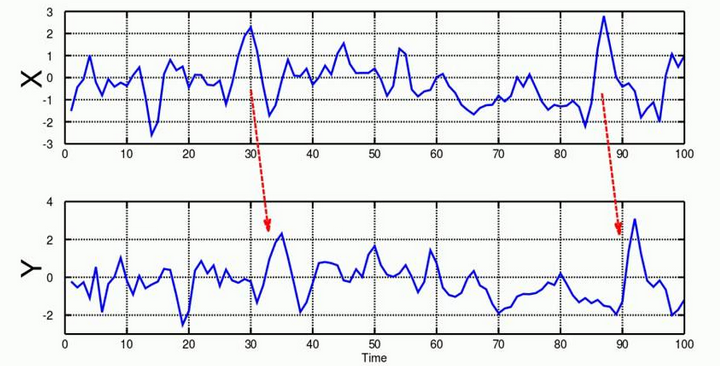
\includegraphics[scale=.6]{GC.png} 
	\end{center} 
	\caption{\textit{Example of signal X Granger-predicting signal Y. }} 
	
\end{figure}

As already mentioned in Section \ref{section 1.5}, observing a correlation between two time series 
is not enough to establish a \textit{relationship} between them. Indeed, a further indicator of  the synchronization between signals is the presence of an underlying \textit{cause-effect} mechanism. If such relationship is found, besides observing a synchronization, one can determine also which signal (and, in this case, mouse) is responsible for causing the opponent's one.\\
In situations like the EEG experiment in \cite{15} % [Novembre et al.]
 discussed in Section \ref{section 1.5}, such relationship is investigated through a manipulations on the experimental level (via \textit{Multi-brain stimulation}). In  the current work, once dealing with data already measured, a different and sophisticated approach is adopted, based on statistical principles: the \textbf{Granger causality}.\\
The Granger causality (\textbf{G-causality}) is a method aimed to identify causal relationship between time series data. The word "casuality" is mainly due to historical reasons, since many debates about its correctness are still ongoing, and it would be probably more precise to refer to it as "Granger \textit{prediction}".
\\

Given two time series $ \textbf{x} = \{x_i\}_{i=1}^N$ and  $\textbf{y} = \{y_i\}_{i=1}^N$, the G-causality method is based on the following scheme:

\begin{enumerate}
	
	\item Generation of a \textbf{vector autoregressive model (VAR)} of order $p$, where $p\ge 1$ is an integer to be determined, for one of the two time series, considering its previous values
	
	\begin{equation}
	\hat{x}_t = a_0 + a_1 x_{t-1} + a_2 x_{t-2} + \dots + a_p x_{t-p} \label{var}
	\end{equation}
	
	
	\item Generation of a second autoregressive model, in which the values of the second series $\textbf{y}$ are added  to  (\ref{var})
	\begin{equation}
	\hat{x}_t = a_0 + a_1 x_{t-1} + a_2 x_{t-2} + \dots + a_p x_{t-p} + b_1 y_{t-1} + \dots + b_p y_{t-p} \label{var2}
	\end{equation}
	
	
	\item Comparison between the two models: if  (\ref{var2}) is more significant  than  (\ref{var}) (in a way to be clarified in the following), then signal $\textbf{y}$ \textit{Granger-predicts} signal \textbf{x} 
	
\end{enumerate}

More formally \cite{19}, % [Barnett-Seth], 
given two stochastic processes $ \textbf{X} = \{X\}_{i=1}^N $ and $ \textbf{Y} = \{Y\}_{i=1}^N $, process Y \textit{does not} G-causes process X if X, conditional its past, is independent by the past of Y. A vector autoregressive model for a process $U$ takes the form

\begin{equation}
\textbf{U}_t = \sum_{k=1}^{p} A_k \textbf{U}_{t-k} + \varepsilon_t \label{Ut}
\end{equation}



where $p$ is the \textbf{order} of the model, $\{ A_k\}_{k=1}^p$ are the \textbf{regression coefficients} and $\varepsilon_t$ the \textbf{residuals}, assumed normally and independently distributed. The \textbf{ residual covariance matrix} of the model is defined as $ \Sigma = Cov(\varepsilon_t) $ and it is assumed to be stationary. The process $U$ can then be identified both as $X$ and $Y$. Given a VAR model of the form (\ref{Ut}), the \textbf{autocovariance sequence} $ \{\Gamma_k\}_{k=1}^p $ is defined as $ \Gamma_k = Cov(\textbf{U}_t,\textbf{U}_{t-k})$, and it is possible to relate this quantity to the autoregression coefficients $\{ A_k\}$ thanks to the \textbf{Yule-Walker} equations \cite{20} %[Anderson,1971]

\begin{equation}
\Gamma_k = \sum_{i=1}^{p} A_i \Gamma_{k-i} + \delta \Sigma \hspace{1 cm }  k = 1, \cdots, p \label{Yule-Walker}
\end{equation}\\

Standard VAR theory \cite{21} %[Hamilton]
 requires the condition $ \sum_{k=1}^{N}||A_k||^2 < \infty $. Moreover, defining the \textbf{characteristic polynomial} as 
$$ \phi_A(z)= \det \left( I - \sum_{k=1}^{p} A_k z^k \right) $$
it must be that the \textbf{spectral radius} $\rho(A) := \max_{\phi_A(z)=0}|z|^{-1}$ is strictly less than $1$, as a \textit{stability} condition.
\\

Considering now a process in which $ \textbf{U}_t = \begin{bmatrix} \textbf{X}_t  \\  \textbf{Y}_t \end{bmatrix} $, its VAR formulation reads

\begin{equation}
\textbf{U}_t = \sum_{k=1}^{p} \begin{bmatrix} A_{xx,k}  &  A_{xy,k} \\  A_{yx,k}  & A_{yy,k} \end{bmatrix} \textbf{U}_{t-k} + \begin{bmatrix} \varepsilon_{x,t}  \\  \varepsilon_{y,t} \end{bmatrix}
\end{equation}


and its residual covariance is $ \Sigma = Cov\left(\begin{bmatrix} \varepsilon_{x,t}  \\  \varepsilon_{y,t} \end{bmatrix}\right) = \begin{bmatrix} \Sigma_{xx}  &  \Sigma_{xy} \\  \Sigma_{yx}  & \Sigma_{yy} \end{bmatrix} $.\\

This augmented formulation contains both the regression models for process $X$ and $Y$. For example, its first component reads

\begin{equation}
\textbf{X}_t = \sum_{k=1}^{p} A_{xx,k} \textbf{X}_{t-k} + \sum_{k=1}^{p} A_{xy,k}  \textbf{Y}_{t-k} + \varepsilon_{x,t}
\end{equation}

If the process $Y$ does not G-cause the process $X$, it follows that the coefficients $\{A_{xy,k}\}_{k=1}^p $ are all equal to $0$, and the model becomes

\begin{equation}
\textbf{X}_t = \sum_{k=1}^{p} A'_{xx,k} \textbf{X}_{t-k} + \varepsilon'_{x,t} \label{G-model}
\end{equation}

Therefore, a statistic test checking  the null hypothesis \{$ H_0:  Y \hspace{0.2cm} \text{does not G-predicts} \hspace{0.2 cm} X $\} has the form

\begin{equation}
H_0: A_{xy,1} = A_{xy,2} = \cdots = A_{xy,p} = 0
\end{equation}


If  $\Sigma'_{xx} = Cov(\varepsilon'_{x,t}) $ is the residual covariance matrix of model (\ref{G-model}), standard theory \cite{22} %[Edwards, 1992]
 suggests the use of the \textbf{(log-)likelihood statistics} to obtain a \textit{maximum-likelihood} estimator of the G-causality between $Y$ and $X$ (here referred as $ \mathcal{F}_{Y \rightarrow X} $):

\begin{equation}
\mathcal{F}_{Y \rightarrow X}  = \ln \frac{det(\Sigma'_{xx})}{det(\Sigma_{xx})} \label{test stat}
\end{equation}


Since the determinant of a covariance matrix (i.e. the \textit{generalized variance}) quantifies the \textit{prediction error} of its regression model, the interpretation of (\ref{test stat}) is that the G-causality statistics  $ \mathcal{F}_{Y \rightarrow X} $ is a measure of how much the prediction error is reduced when also the process $Y$ is included in the regression model. Clearly, this same procedure applies to the statistics  $ \mathcal{F}_{X \rightarrow Y} $, in which the directionality of the relationship is inverted. It can be proven \cite{23} %[Wilks \& Wald]%
 that, under the null hypothesis, $ (N-p)\mathcal{F}_{Y \rightarrow X} \sim \chi^2(d)$, where $ d = pN^2$.
\\
To summarize, the typical workflow for G-causality estimation, consists in the following steps:

\begin{enumerate}
	\item Estimatation of the model order $p$ via appropriate criterion (such as AIC and BIC)
	
	\item Estimatation of the autocovariance sequence $\Gamma_k$ and the VAR coefficients $(A_k, \Sigma)$ through the Yule-Walker equations (\ref{Yule-Walker}), both for reduced and augmented models. Verify that $ \sum_{k=1}^{N}||A_k||^2 < \infty $ and  $\rho(A) < 1$
	
	\item Computation of the G-statistics $ \mathcal{F}_{Y \rightarrow X} $ and $ \mathcal{F}_{X \rightarrow Y} $ through (\ref{test stat})
	
	\item Evaluation of the significance of the statistical tests against the null hypotesis, computing the $p$ -values of the two tests 
	
\end{enumerate}





\newpage
\chapter{Interbrain data analysis: emotion discrimination task}

In this chapter, the main results on the data analysis for the emotion discrimination task are presented. After describing the phases of the task and identifying the appropriate way  to represent the data through normalization, a first set of considerations on the neural activity of mice, in relation to their behaviour, are taken into account. Then, the focus goes to the main part of the analysis: the \textit{Interbrain synchrony} among neural activities. The different concepts of synchrony introduced in Chapter 2 are  investigated, i.e. the cross-correlation between the mean activities of the mice and the peak synchronization among neurons. Finally, the topic of causality between signals is dealt using the tool of Granger prediction.\\
All the results refer to two versions of the emotion discrimination task: a standard task, where the observer is in a \textit{neutral condition}, and the \textbf{self-experience task}, in which the observer has been stressed before the task.


\section{Emotion discrimination task}

\begin{figure}[H]
	\begin{center}
		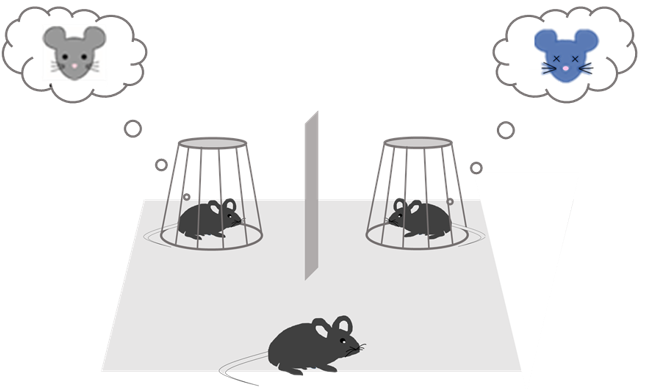
\includegraphics[scale=.65]{emotion_discrimination.png} 
	\end{center} 
	\caption{\textit{Scheme of the emotion discrimination task.}} \label{edt}
	
\end{figure}

In the \textit{emotion discrimination task}, an \textbf{observer} mouse is facing two \textbf{demonstrators} in an open arena, as shown in Figure \ref{edt}. One demonstrator is in a \textit{neutral} state, the other in a \textit{stressed} state, meaning that it has been subjected to a \textit{stress protocol} (forced restrainment) before the test. The task consists of three main parts:

\begin{enumerate}
	
	\item \textbf{Homecage restrainment}: the three mice are kept separate in their cages in normal conditions. \\
	$\longrightarrow$ \textit{Duration}: 5 minutes
	
	\item \textbf{Habituation}: the observer mouse is free to move in an empty open arena; in the meantime the neutral demonstrator is kept in the cage, while the stressed demonstrator is being subjected to the stress procedure. \\
	$\longrightarrow$  \textit{Duration}: 15 minutes
	
	\item \textbf{Test}: the demonstrators join the observer in the arena. Only the observer is free to move, since the two demonstrators are kept behind a cage allowing sight, sniffing but no direct contact. \\
	$\longrightarrow$  \textit{Duration}: 15 minutes
\end{enumerate}

During all the three phases, the neural activities of the three mice are recorded via microendoscopic calcium imaging, as described in Section \ref{section 1.3}, in which the target is the set of \textit{somatostating-expressing} interneurons in the anterior cingulate cortex (SOM+ in the ACC, Section \ref{first section}). Moreover, the position of the observer mouse along time is recorded during habituation and test phases, and TTL signals (binary recordings of events) of the reciprocal sniffing between one observer and  demonstrators have been recorded during the test. Finally, spatial data of the neurons in the \textit{region of interest (ROI)} captured by the miniscope, are available as well, such as their position and size.\\
These types of data can lead to several analyses:
\begin{itemize}
	
	\item Inspecting if there exist correlations among the neural activity levels of one mouse and what is happening during the task, such as the stressing procedure, proximity or sniffing between two mice
	
	\item Testing the presence of \textit{activity synchronization} among the neural signals of two mice, as described in chapter 2, in relation to what is happening in the test (proximity of two subjects, sniffing)
	
	\item Investigating whether the activity in one mouse is \textit{predicting} the activity in another, for example via  Granger causality analysis introduced in Section \ref{section granger}
	
	\item Investigating whether the neuronal firing in single mice seems to follow \textit{patterns}, or if it is possible to predict mathematically such chain of events (problem dealt in chapter 6)
\end{itemize}


The analyses involve two types of data: in the first one, a neutral observer interacts with the demonstrators, while the second one investigate the so called \textbf{self-experience} setting, in which, before the test, also the observer is subjected to a stress protocol. For each one of the two cases, two triplets of mice have been tested with the same procedure, and the results have been averaged among them.\\
It is worth to observe that the phases of homecage and habituation play the role of a \textit{control} in the data analysis: given a quantity measured from the data of calcium concentrations (such as the level of synchronization), we can assume that a result is significant, and thus related to the interaction between mice, if it is present in the test phase but not in the control phases of homecage and habituation, in which the mice cannot interact and are located in different places.

\section{Normalization of the dataset} \label{norm}


\begin{figure}[H]
	
	\begin{center}
		\hspace*{-1cm}
		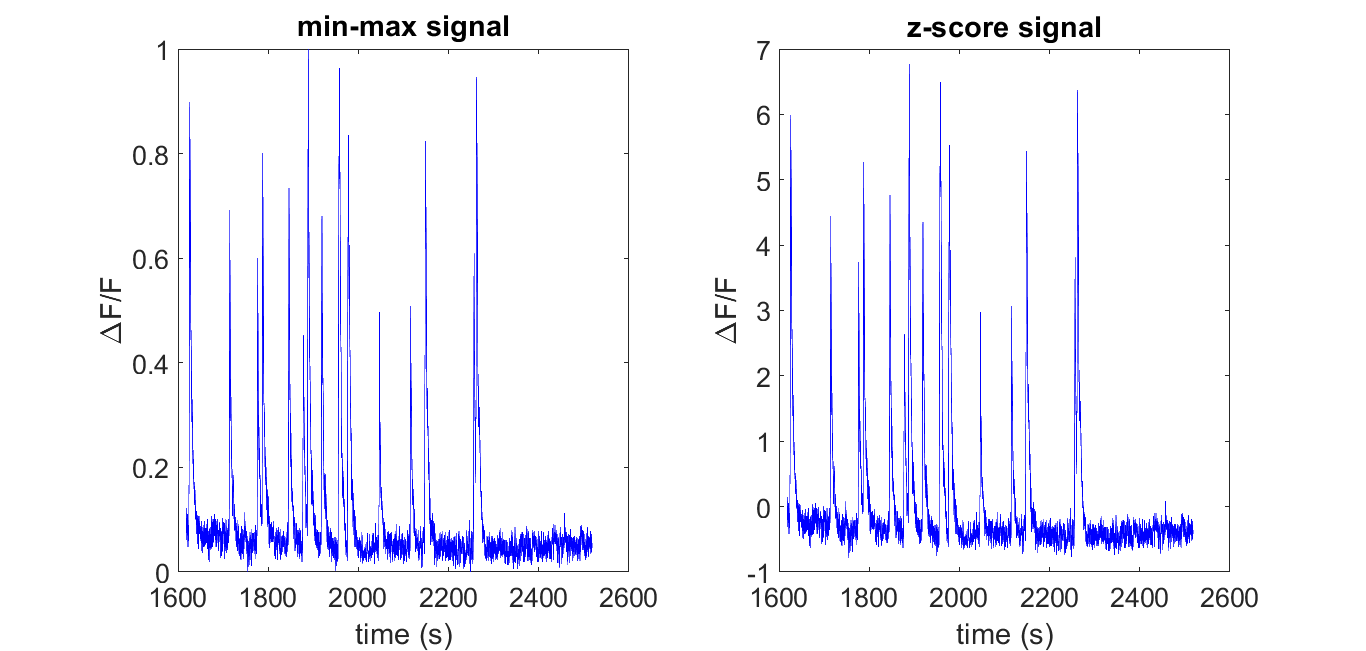
\includegraphics[scale=.47]{normalizations.png} 
	\end{center} 
	\caption{\textit{Different normalizations of the signal. Left: min-max normalization, in which the signal assumes values in $[0,1]$. Right: z-score normalization, with no constraint on the scale of the $y$-axis. }}
	\label{normalizations}
\end{figure}

The main object of the analysis is given by the calcium signals recorded in every single neurons, expressed in terms of relative fluorescence $\frac{\Delta F}{F}$. Such signals can be subjected to operations and comparisons, either among neurons of a single mouse, or among activities in different mice. Based on this scenario, it necesessarily follows that it is fundamental to choose a proper \textit{normalization} of the data which can allow such processes. The literature proposes several ways to treat data, (see Figure \ref{normalizations}):

\begin{enumerate}
	
	\item \textbf{Raw approach}. The raw data, coming from the Inscopix pre-processing described in Section \ref{section 1.3}, are usually not ready to be analyzed yet. Although processes of normalizations on the ROI videos, filtering and noise detection  have been already performed, the single information of a fluorescence value $\frac{\Delta F}{F}$ needs to be treated carefully. Every single neuron is characterized by a baseline activity, alternated with rapid and huge spikes. Such baseline value, which biologically represents the \textit{non activity} of a neuron, can take different values across different neurons. Moreover, the values reached by the spikes can appear in different magnitudes, but this does not necessarely reflect  what is really happening in the reality: a spike may exhibit smaller amplitudes for the simple fact that less GCaMP protein, which reacts with calcium and emits flourescence, was present at that moment, and consequently the spiking of that neuron assumed smaller values. 
	
	\item \textbf{Min-max normalization}. With the min-max normalization, every value $x_t$ of the signal $ x = \left\{ x_t\right\}_{t=1}^N$ at time $t$ is normalized through
	
	\begin{equation}
	x_t^{mm} = \frac{x_t -  \min(x)}{\max(x) - \min(x)}
	\end{equation}
	
	With the min-max normalization, all the signals are bounded in the interval $[0,1]$, where the values $0$ and $1$ occur in correspondence of the lowest and  highest values, respectively. Therefore, using this normalization, all the signals are treated in the same way, since they are all in the same interval, whatever their original value and scale was in the raw dataset.
	
	\item \textbf{$Z$-score normalization}. For a value  $x_t$ of the signal $ x = \left\{ x_t\right\}_{t=1}^N$, the z-score normalization reads. 
	
	\begin{equation}
	x_t^{z} = \frac{x_t -  \mu}{\sigma}
	\end{equation}
	
	where $\mu$ and $\sigma$ are the mean and standard deviation of the signal, respectively. The goal of this normalization is to obtain signals with $0$  mean and unitary standard deviation, making them comparable without constrains on their values, as in the case of the min-max normalization. For this reason, $z$-score is the most used type of normalization in the literature.
	
	
\end{enumerate}


All the different normalizations do not modify the shape of the signals, but their \textit{scale}. As for this work, we chose a modification of the $z$-score normalization, defined as \textbf{$z$-score on baseline}, in which signals are aligned and then divided by their standard deviations. Therefore, the proposed approach belongs to the $z$-score case, but the alignment is not performed on the mean of each signal, but on their baseline activities. The reason for this is that two signals coming from neurons, when subtracted by their own mean, can still exhibit different values of the baseline. Therefore, with the chosen normalization the alignment is done on such baselines, which are set to $0$ for every neuron, and operations on signals, such as sum or direct comparison, can become meaningful.



\section{Behavioural analysis of the task}


\begin{figure}[H]
	
	%\begin{center}
	\centering
	
	\hspace*{-1 cm}
	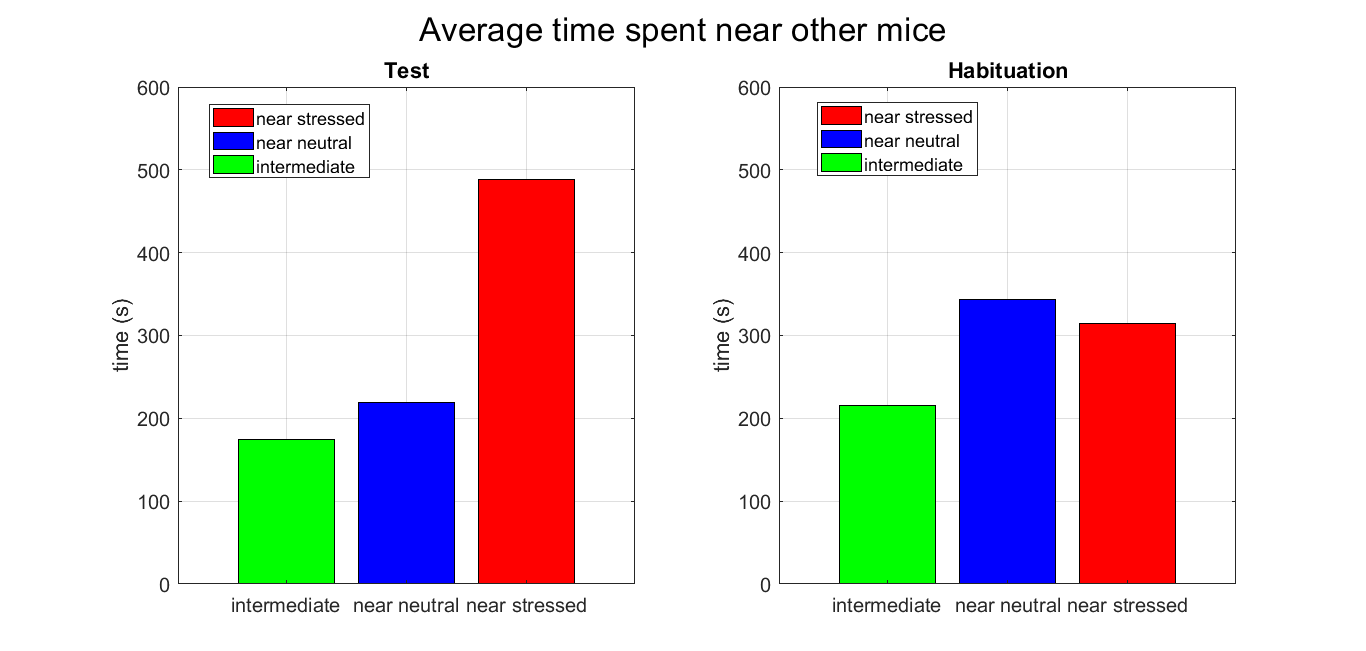
\includegraphics[scale=.45]{times.png} 
	%\end{center} 
	\caption{\textit{Average time spent by the observer near the demonstrator cages, or in the intermediate area. Left: results during the test. Right: results during the habituation. }} \label{times}
	
\end{figure}

In \cite{8}, the same neuronal population, namely the somatostin interneurons, was observed during a task following a protocol similar to the current emotion discrimination task. In that case, however, the area of interest was the medial prefrontal cortex, and the main focus on the electrophyisiological activity. As results, it was evident that the observer mouse spent more time near the stressed demonstrators, and its neural activity (in terms of action potentials) showed higher values during those periods.\\
In this work, we obtained the following results:

\begin{itemize}
	\item The observer spent a significantly higher time near the stressed demonstrators, rather than near the neutral one or in an intermediate zone (see Figure \ref{times}). Moreover, in order to rule out the possiblity that this effect was due to spatial factors present in the cage where the stressed mouse was located, a comparison with the habituation has been performed. During the habituation, the observer is free to move in the arena for the same time as in the test, but in the arena the two cages for the demonstrators are empty. The results show clearly that in this situation the observer doesn't show a particular tendency for proximity, and in particular spends considerably less time near the cage of the stressed mouse.
	
	\item In the analysis of the calcium activity, no evidence of correlation between activity  and proximity to demonstrators seemed to emerge during the test: from the recorded neurons, the observer maintains an overall similar average activity through the different areas of the arena. As for the demonstrators, only the neutral appears to show an increase activity during the sniffing with the observer (Figure \ref{activity_barplot}).
	\\
	
	Next, a comparison on the average activity of mice during the phases of the task have been taken into account (see Figure \ref{activities}). The results showed that, in general, the mean activity seems to be higher during the habituation. This happens in particular for the stressed mouse, coherently with the fact that during the habituation, it is  subjected to the stress protocol (forced restrainment), for which it is expected to show higher activity. Overall, the neutral mouse shows smaller values of calcium activity, during both habituation and test, compared to the observer and the stressed conspecifics.
	
\end{itemize}


\begin{figure}[H]
	
	\begin{center}
		\hspace*{-1.cm}
		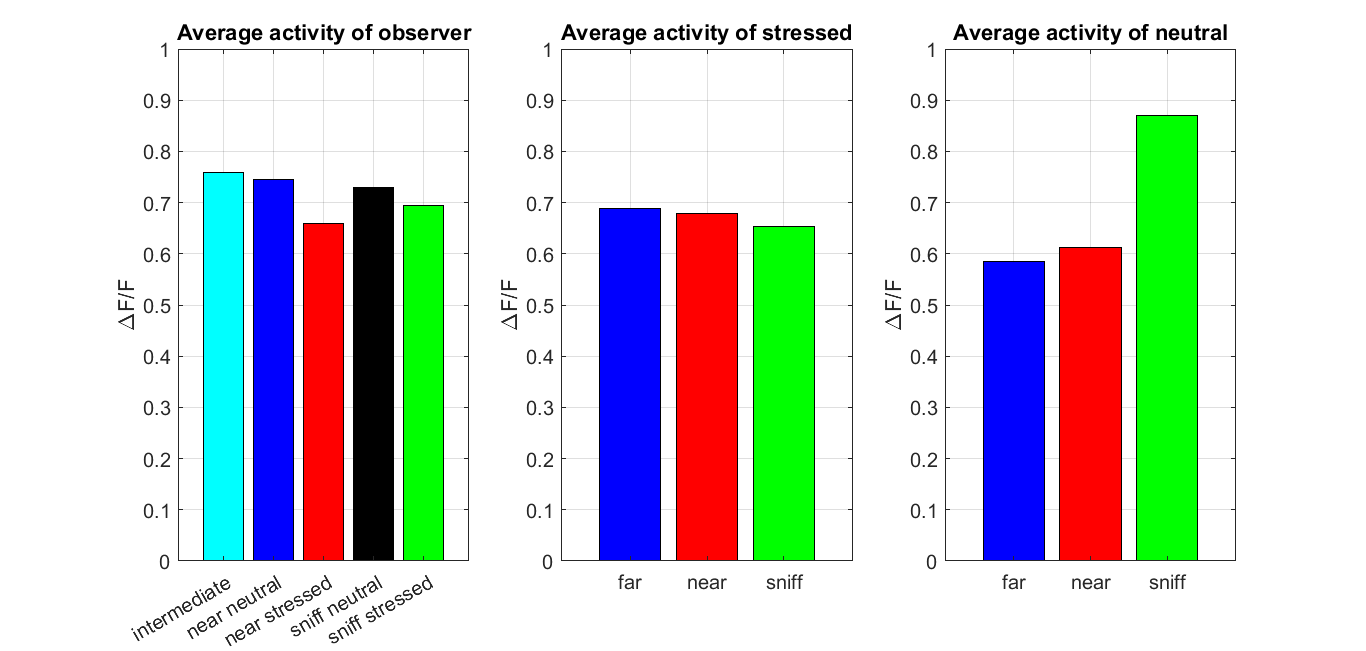
\includegraphics[scale=.47]{activity_barplot.png} 
	\end{center} 
	\caption{\textit{Average activity of the mice during the test. Left: observer. No tendencies seem to emerge when it is in intermediate area, close to demonstrators or sniffing with demonstrators. Center: stressed.  Right: neutral.}} \label{activity_barplot}
	
\end{figure}


\begin{figure}[H]
	
	\begin{center}
		
		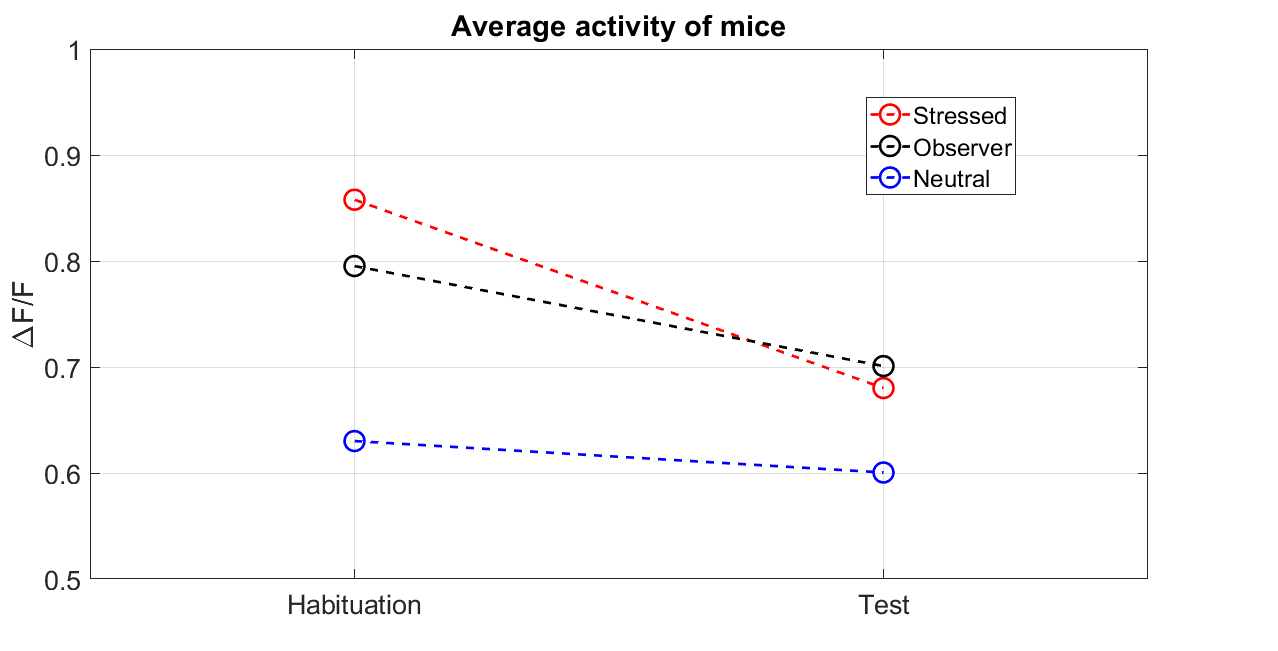
\includegraphics[scale=.45]{activities.png} 
	\end{center} 
	\caption{\textit{Evolution of the average activity of the three mice from the habituation to the test.}}
	\label{activities}
\end{figure}


\section{Cross-correlation analysis for the mean activity}

\begin{figure}[H]
	
	\begin{center}
		\hspace*{-1.4cm}
		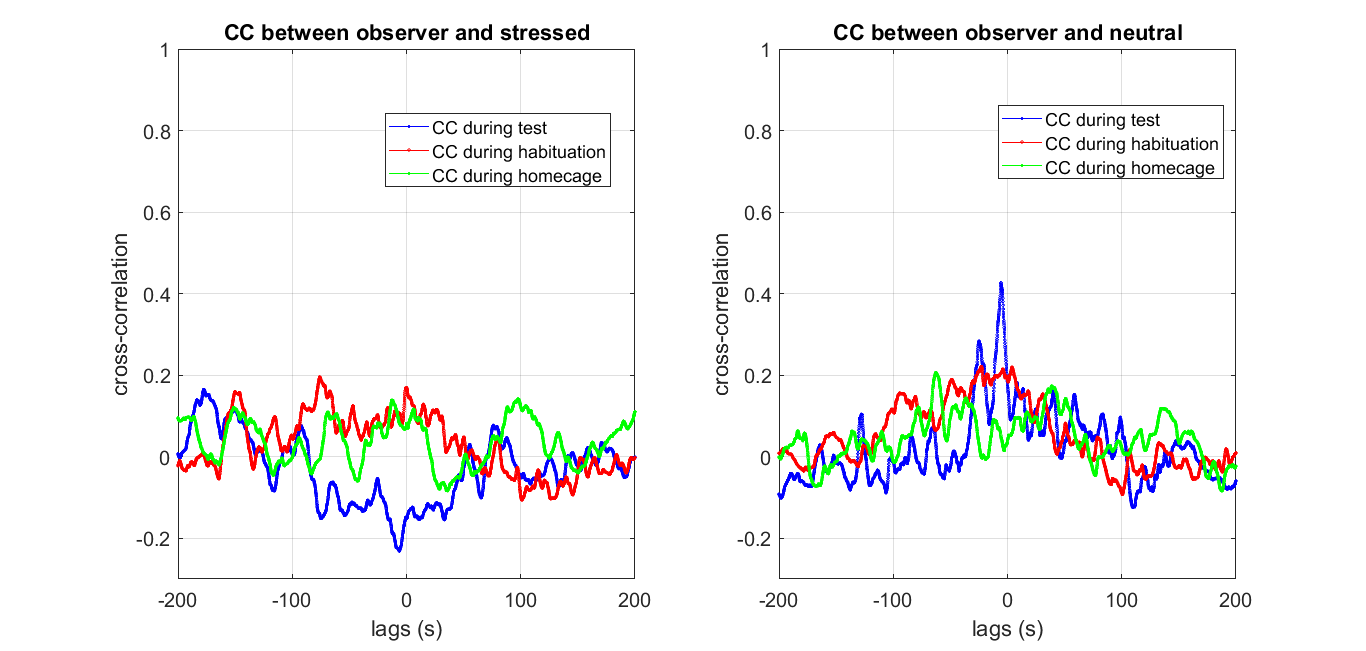
\includegraphics[scale=.5]{average_cc.png} 
	\end{center} 
	\caption{\textit{Left: average cross-correlation between observer and stressed. Right: average cross-correlation between observer and neutral.}} \label{cc}
	
\end{figure}

With the \textit{Interbrain analysis}, we study whether the interactions between two mice are followed by a synchronization of their neural activities. As explained in Section \ref{cc_section}, one of the main tools for the synchronization analysis is the \textbf{cross-correlation}.\\
As first step, following the approach of \cite{16}, every mouse has been gifted with its \textit{overall activity}, consisting in a mean of the activities of all its recorded neurons. The spatial data on the position of the observer in the arena during habituation and test, made it possible to divide such mean activities in several parts::

\begin{enumerate}
	\item Restriction to the times of proximity between the observer and the stressed
	\item Restriction to the times of proximity between the observer and the neutral
	\item Restriction to the times of reciprocal sniffing between two mice
\end{enumerate}

The above subdivision allows us to analyze the correlation among the activities of two mice when they are actually close to each other. In this context, a cross-correlation analysis on the mean activity has been performed, comparing what happens during the homecage, habituation and test. During homecage and habituation phases, the three mice are kept separate. Therefore, inspecting the correlation among the activites during these phases is a useful \textit{control}, i.e. a case of comparison in order to see what to expect when correlation should not be present.
\\

After computing the mean of all the $\frac{\Delta F}{F}$ signals in each neuron for every mouse, and applying the above classification $1.-3.$, the cross-correlation between observer and stressed and between observer and neutral mean activies has been computed, as described in Section \ref{cc_section}. As shown in Figure \ref{cc}, analyzing the average cross-correlation between the two experiments, one can notice the presence of a peak around $ lag=0 $ for the pair observer-neutral in the test phase. This tendency is not present in the control cases of habituation and homecage, making it a proper feature of the test. On the other side, the cross-correlation between observer and stressed does not show any particular difference with respect to the homecage and habituation phases. A further verification has been given by observing the cross-correlation between the observer and one demonstrator, but considering the periods when the observer was visiting the opposite demonstrator. As a result, the cross-correlation between observer and neutral is inhibited considering the instants when the observer was visiting the stressed, and the cross correlation between observer and stressed remains non significant when the observer is visiting the neutral (Figure \ref{distant}).\\
 Overall, these results may show the presence of a synchronization between neural activities of the observer and the neutral demonstrator, but not between the observer and the stressed one, and this effect is present only during the test and during the proximity of the two mice.

\begin{figure}[H]
	
	\begin{center}
		\hspace*{-1.4cm}
		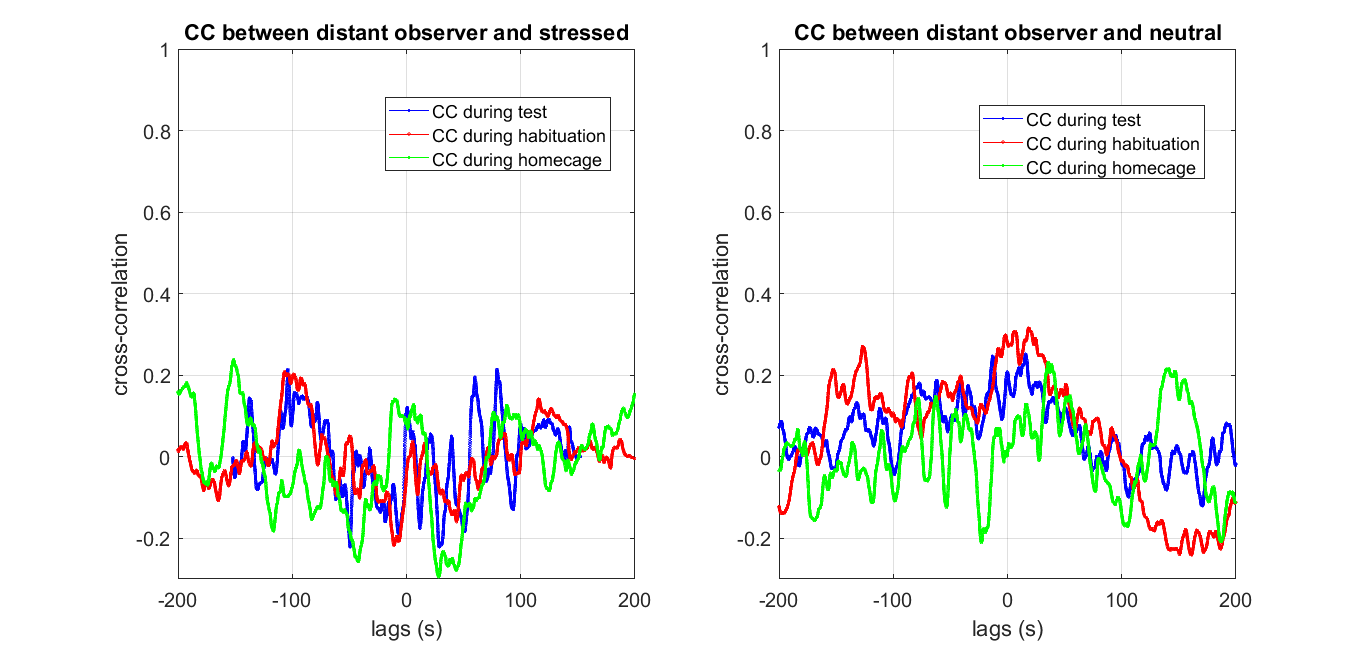
\includegraphics[scale=.5]{cc_distant.png} 
	\end{center} 
	\caption{\textit{Left: average cross-correlation peaks between observer and stressed when the observer is visiting the neutral. Right: average cross-correlation peaks between observer and neutral when the observer is visiting the stressed.}} \label{distant}
	
\end{figure}


Then, two particular cases have been considered: the sniffing interactions and the restriction to the first part of test (first 2 minutes of the test). The sniffing is known to be one of the most direct interactions that two mice can display between each other, and therefore is of a particular interest for what could happen at synchronization level. The restriction to the first two minutes of the test is of interest based on previous results \cite{16}, which show that the first period of interactions among mice is the one which determines some most relevant neural tendencies, such as the display of synchronization.\\
The obtained results allowed us to draw the following conclusions (Figure \ref{initial}):

\begin{itemize}
	\item Data measurements during the sniffing interactions are coherent with those obtained during the whole test: a peak around $lag=0$ is present only in the cross correlation computed between observer and neutral, but not between observer and stressed
	
	\item Consistent with previous results, the peak of cross-correlation between observer and neutral is higher if we restrict the analysis to the first two minutes of interaction.
	
\end{itemize}

A summary of the cross-correlation results can be seen in Figure \ref{cc_average}. For every case, the values refer to the cross-correlation peak recorded around $lag=0$. While for the observer-stressed case no significant differences arise, between observer and neutral the test phase shows higher correlations, in particular in the sniffing and at the beginning of the test.



\begin{figure}[H]
	
	\begin{center}
		\hspace*{-1.4cm}
		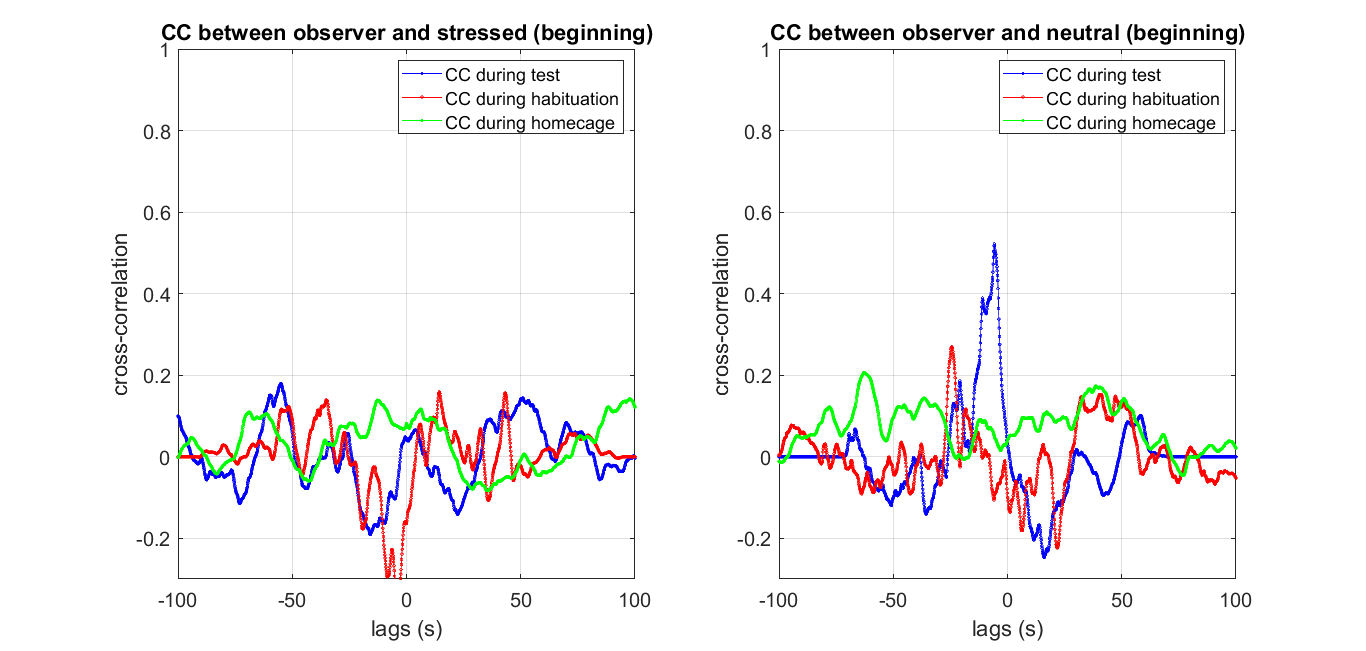
\includegraphics[scale=.5]{average_cc_initial.png} 
	\end{center} 
	\caption{\textit{Left: average cross-correlation between observer and stressed, during the first two minutes of test. Right: average cross-correlation between observer and neutral, during the first two minutes of test.}}
	\label{initial}
\end{figure}

\begin{figure}[H]
	
	\begin{center}
		\hspace*{-1.4cm}
		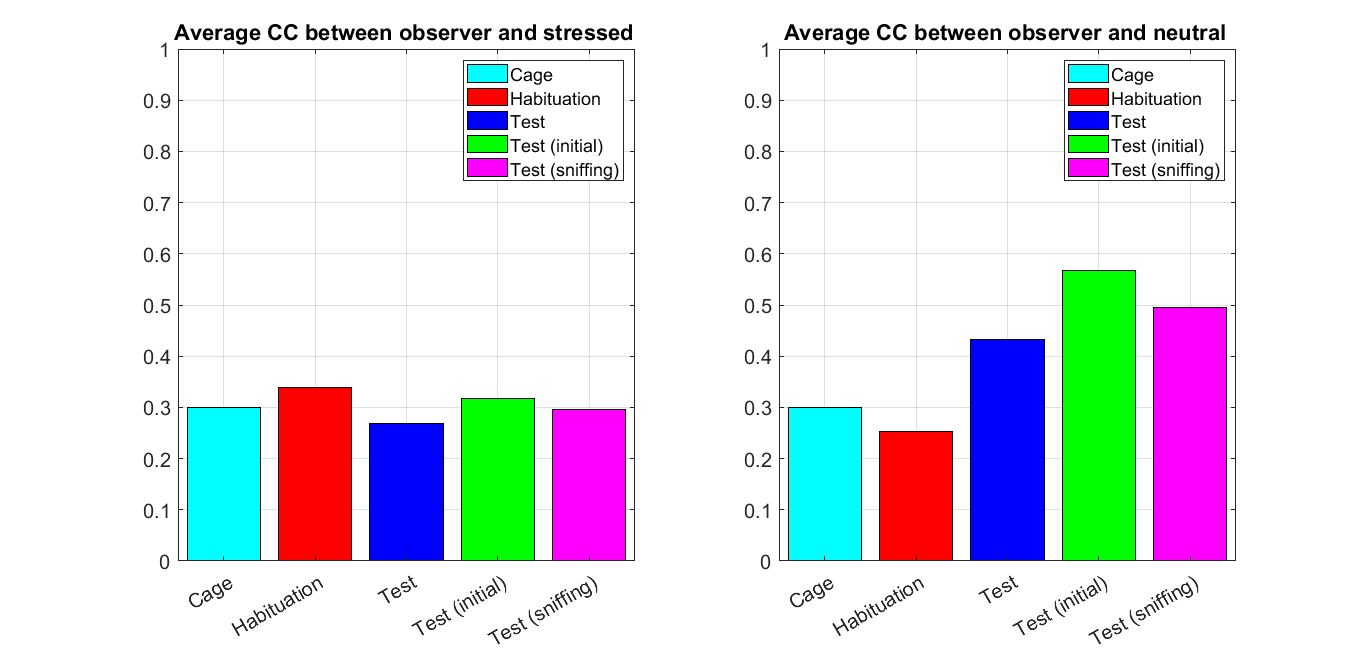
\includegraphics[scale=.5]{cc_average.png} 
	\end{center} 
	\caption{\textit{Left: average cross-correlation peaks between observer and stressed. Right: average cross-correlation peaks between observer and and neutral.}}
	\label{cc_average}
\end{figure}



\section{Peak synchronization analysis}

\begin{figure}[H]
	
	\begin{center}
		\hspace*{-1cm}
		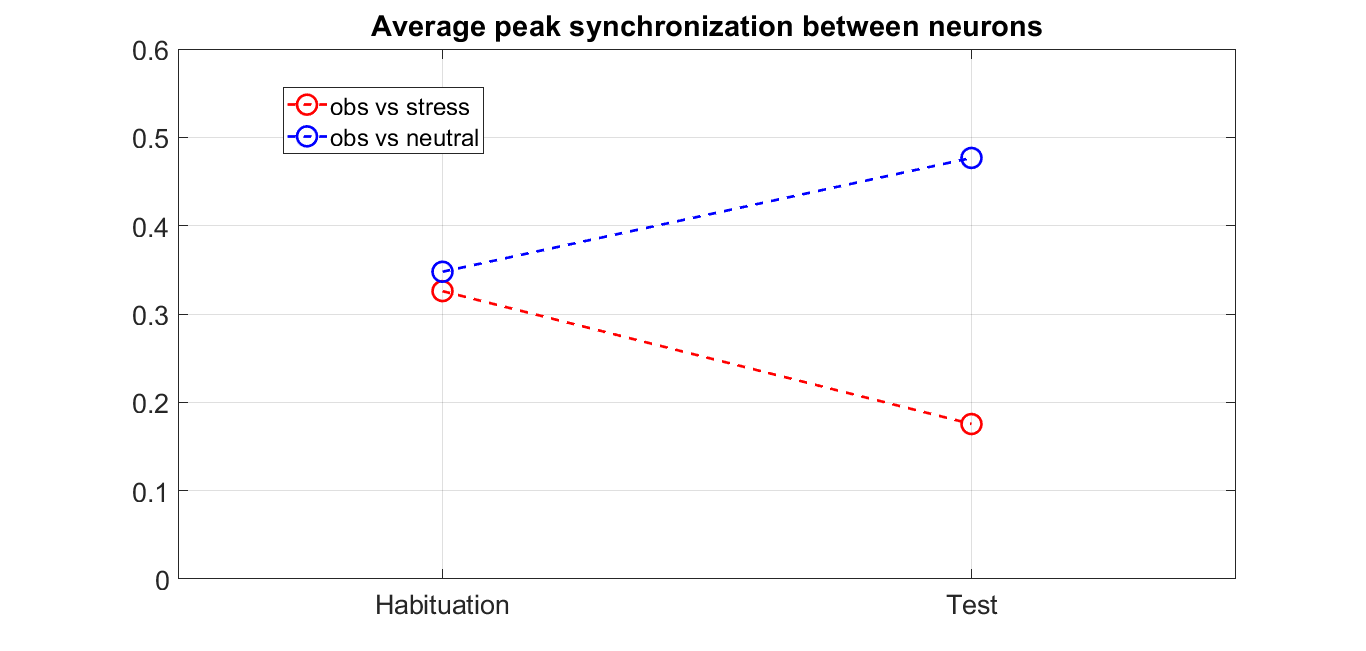
\includegraphics[scale=.45]{avg_pks.png} 
	\end{center} 
	\caption{\textit{Evolution of the average peak synchronization index from the habituation to the test, for the cases observer-stressed and observer-neutral.}} \label{avg_pks}
	
\end{figure}

From the mean activity of the mice, the focus goes now to single neuron synchronization. As presented in Section \ref{section 2.3}, a useful tool to quantify the degree of simultaneous firing between two neurons is given by the \textbf{peak correlation index} (\ref{peak index}), which takes into account the number of simultaneous peaks observed during a synchronization time window $dT$ between two signals. As for the present work, the chosen time window, in which two peaks are considered simultaneous, has been set to $dT = 1 s$. The analysis of peak correlation proceeds according the following steps:

\begin{enumerate}
	
	\item Computaton of the peak correlation index for every pair of neurons between the observer and one demonstrator 
	
	\item Computation of the average of the indices for a couple of mice during the test, to be confronted with the same average obtained during the habituation. In this way we can compare the change in simultaneous firing between two neurons from one phase of the task to the other
	
	\item The result on the evolution of the mean correlation index is accompanied by a \textit{one-way ANOVA} test \cite{17} on the significance of the difference between the two groups of indices. The null hypothesis of the ANOVA states that there is no significance in the difference between the two pupulations, i.e. that $ \mu_1 = \mu_2$,  $\mu_1$  and $ \mu_2$ being the  means of the two populations. Such hypothesis is \textit{rejected} for low $p$-values of the associated test.
	
\end{enumerate}

The obtained results are shown in Figure \ref{avg_pks}. Consistently with the cross-correlation results for the mean activity, the average peak correlation index shows higher values in the test, rather than in the habituation, only for the observer-neutral pair, while for the observer-stressed pair it actually decreases. This average result is consistent between all the two investigated datasets, and in both cases the difference between the indices computed in the test and the ones computed in the habituation is significant ($p$-values of $p = 0.0025$ and $p = 0.0128$ for the two datasets from the ANOVA test)


\section{Granger causality analysis}

Granger analysis has been performed in accordance to Section \ref{section granger}, to investigate whether the activity of one mouse is Granger-predicting the activity of another one. This analysis consists in two statistical tests with null hypothesis
$$ H_0:  Y \hspace{0.2cm} \text{does not G-predicts} \hspace{0.2 cm} X $$
where in this case $X$ and $Y$ represent the mean activities of the observer and one demonstrator, respectively. In the two analyzed datasets, the results of the tests, in terms of $p$-values, are summarized in Table \ref{Granger table}. Some considerations are in order:

\begin{itemize}
	\item In the first dataset, there is significance to conclude that the observer activity is G-predicting the demontrator ones (both stressed and neutral), while in the second dataset there is evidence only for the prediction from observer to stressed
	
	\item In all cases, it seems that,  when the observer is visiting a demonstrator, the same demonstrator is influenced by the observer, which G-predicts its activity, i.e. the \textit{directionality} of the prediction goes from the observer to the demonstrator
	
	\item The only coherent result is the one involving the stressed demonstrator, whose activity is always G-predicted by the observer one. However, more data should be available in order to draw more definitive conclusions
\end{itemize}



\begin{table}[H]
	\begin{center}
		\begin{tabular}{ |c|c|c|c| } 
			\hline
			\textbf{Dataset} & \textbf{Directionality} & \textbf{p-value} \\
			\hline
			First & observer $\rightarrow$ stressed & $p = 0.02$ \\ 
			\hline
			First & observer $\rightarrow$ neutral & $p = 0.005$ \\
			\hline
			Second & observer $\rightarrow$ stressed & $p  =  0.01$ \\
			
			\hline
		\end{tabular}
		
	\end{center}
	\caption{\textit{Results of the Granger analysis.}} \label{Granger table}
\end{table}



\section{Self-experience task}


\begin{figure}[H]
	
	\begin{center}
		\hspace*{-1.4cm}
		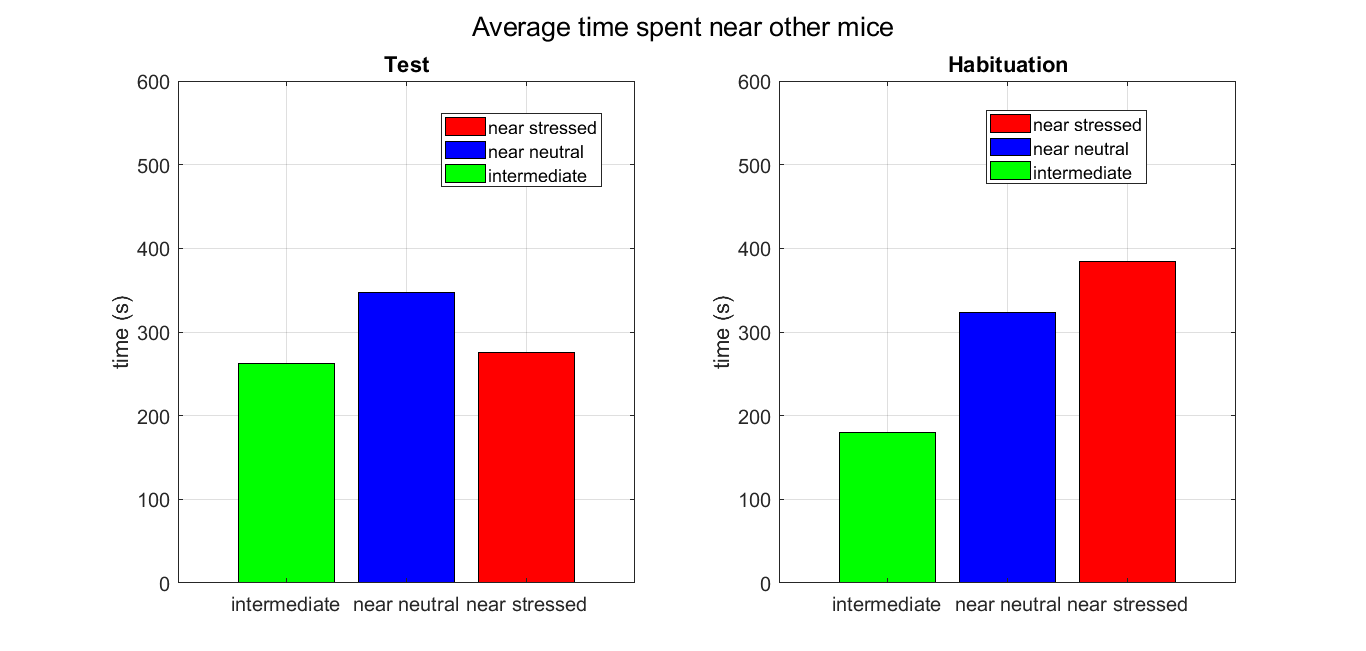
\includegraphics[scale=.5]{times_self.png} 
	\end{center} 
	\caption{\textit{Average time spent by the observer near the demonstrator cages, or in the intermediate area, for the self-experience task. Left: results during the test. Right: results during the habituation.}}
	\label{times_self}
\end{figure}


Two more datasets of the emotion discrimination task have been analyzed. This time, however, they refer to the \textbf{self-experience} configuration, in which the observer has been stressed before the task. The same analyses with the same data normalization as in the standard configuration have been performed. The obtained results are the following:

\begin{itemize}
	\item The observer spends, on average, less time near the stressed, compared to the standard case of non-stressed observer (see Figure \ref{times_self}). This is consistent with an \textit{avoidance} behaviour between two stressed individuals, already observed in past studies \cite{24} %[Ayash]
	
	\item As for the average activity displayed by the three mice, no relevant differences seem to emerge with respect to the standard case. Once again, the strongest activity is observed during the sniffing between observer and neutral (Figure \ref{activity_barplot_self})
	
	\begin{figure}[H]
		
		\begin{center}
			\hspace*{-1.2cm}
			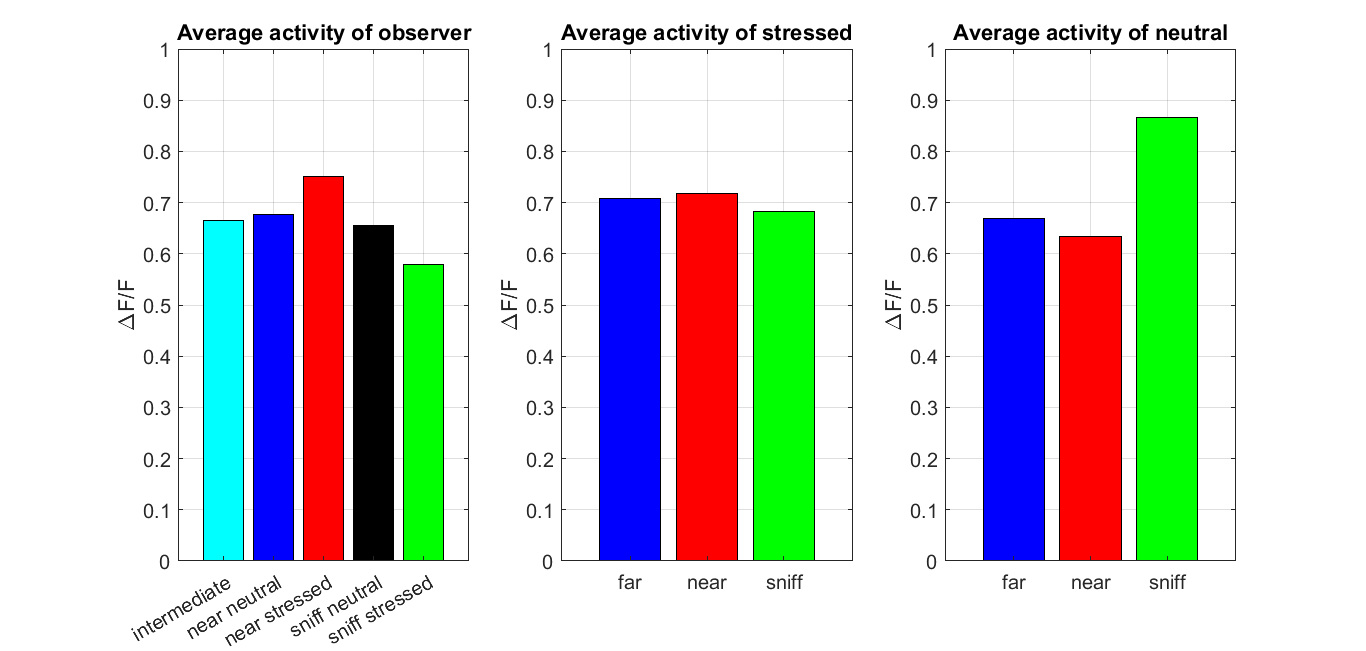
\includegraphics[scale=.48]{activity_barplot_self.png} 
		\end{center} 
		\caption{\textit{Average activity showed by the mice in the self-experience task. Left: observer. Center: stressed. Right: neutral.}}
		\label{activity_barplot_self}
	\end{figure}
	
	\item The cross-correlation peak, observed in the standard case between observer and neutral as shown in Figure \ref{cc}, now is not present. For both analyzed datasets of self-experience type, no correlation seems to emerge between any pair of mice, not even considering the first two minutes of the task (Figure \ref{average_cc_self})
	
	\begin{figure}[H]
		
		\begin{center}
			\hspace*{-1.4cm}
			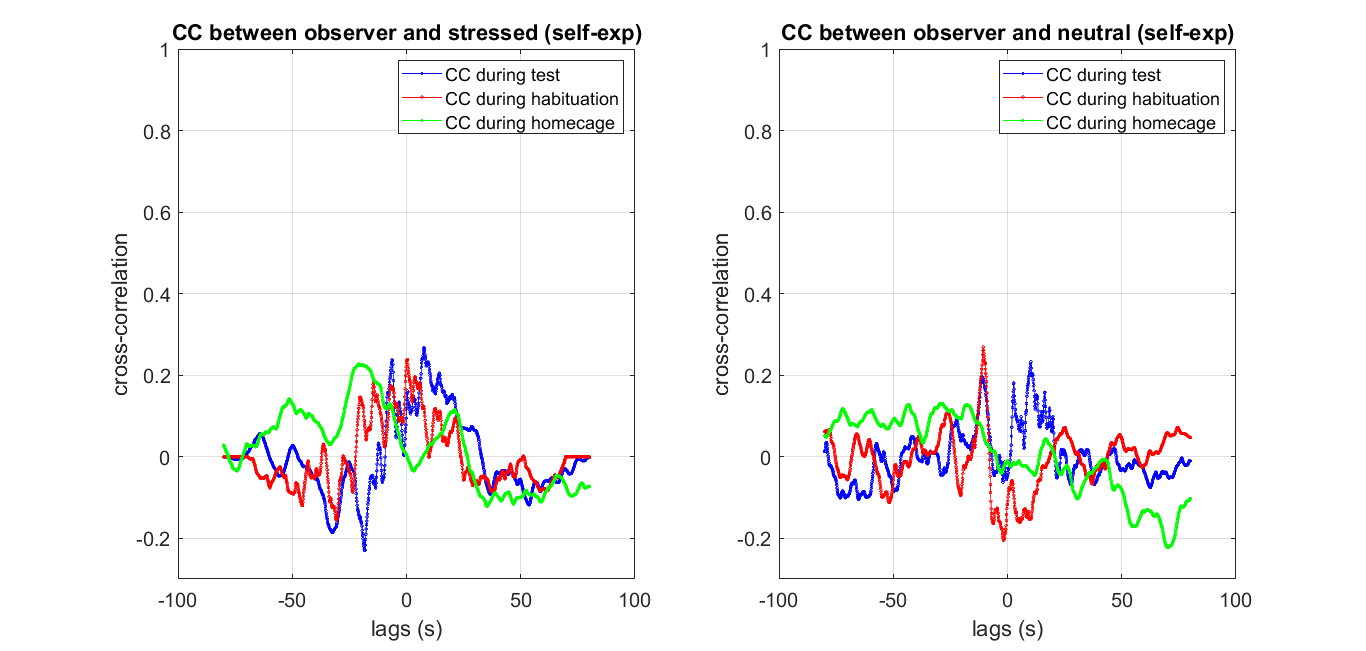
\includegraphics[scale=.5]{average_cc_self.png} 
		\end{center} 
		\caption{\textit{Average cross-correlation, during the first two minutes, in the self-experience task. Left:  between observer and stressed. Right: between observer and neutra.l}}
		\label{average_cc_self}
	\end{figure}
	
	\item The average correlation index slightly decreases in the observer-neutral case and increases in the observer-stressed. These results, however, do not show significance to the ANOVA test (Figure \ref{avg_pks_self})
	
	\begin{figure}[H]
		
		\begin{center}
			\hspace*{-1cm}
			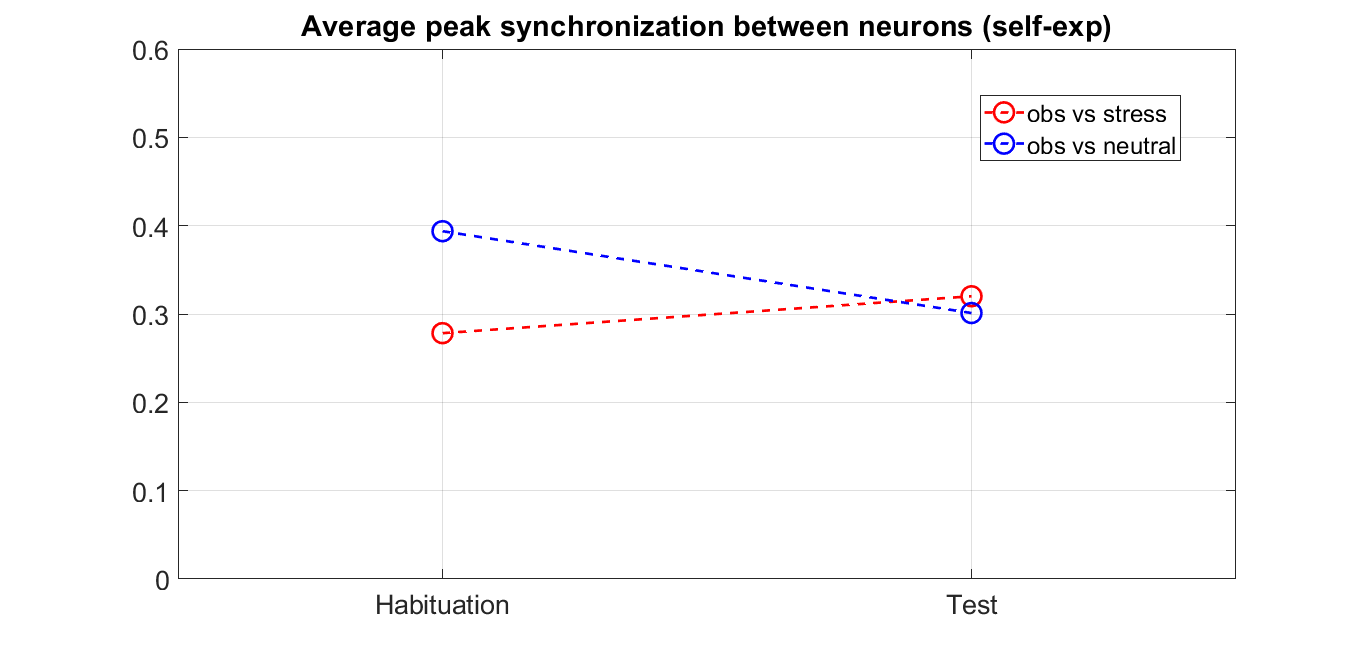
\includegraphics[scale=.45]{avg_pks_self.png} 
		\end{center} 
		\caption{\textit{Evolution of the average peak synchronization index from the habituation to the test, for the  observer-stressed pairs and observer-neutral, in the self-experience task.}}
		\label{avg_pks_self}
	\end{figure}
	
	
	\item Concerning the Granger analysis, in both the analyzed datasets, no significance of Granger prediction in any directionality has been found, both for observer-neutral  for observer-stressed pairs
	
\end{itemize}


\section{Conclusions on the emotion discrimination task}


The analyses on the available data (two experiments performed in the standard configuration, two in the self-experience configuration), suggest the manifestation of some unified tendency in the results, and allow us to make some conclusive considerations:

\begin{itemize}
	
	\item The relevant factor explaining the onset or inhibition of the synchronization among neural activities of SOM+ interneurons in the ACC, seems to be the \textit{stress condition}. Indeed, in the standard emotion discrimination task, a higher synchronization of mean neural activities appears between observer and neutral mice, but not observer and stressed, such as in the peak synchronization between neuron pairs. On the other side, when the observer itself is in a stress condition, also the results with the neutral demonstrator are not present, and the other analyses are less significant. This indicates that a stressed mouse may loose the ability to synchronize
	
	\item In order to have credibility, such conclusions need to be repeated in more experiments to be analyzed, since the consistency observed so far only refer to a small dataset
	
	\item In any event, the conclusions do not apply to the whole brain activity of mice. Rather, the conducted analyses consider a very specific neuronal population in a very specific area ( SOM+ neurons in the ACC). It is possible, and actualy plausible, that different areas and different neurons show a different response in activity synchronization
	
\end{itemize}





\newpage
\chapter{Activity of amygdala in altruistic decision making}

In this chapter, a new aspect of the behavioural analysis from in vivo tasks on mice will be investigated: the ability of mice to display selfish or prosocial choices towards other individuals.\\
Through the \textit{altruism task}, two mice are put in a situation in which they can choose whether to perform an altruistic or selfish choice, while having their neural activity recorded. In this context, however, the employed technique for calcium imaging is not microendoscopic calcium imaging, but \textit{Fiberphotometry} (discussed in Section \ref{section 1.4}), from which an overall signal for the calcium activity is obtained.\\
As for the area of the brain under investigation, in this case the focus is on the \textbf{basolateral amygdala (BLA)}, which has been shown to be connected with prosocial choices in rodents (as anticipated in Section \ref{first section}).\\
While, in the first sections, the task and its main behavioural results are presented, the present contribution to the altruism task is addressed in Section \ref{section 4.5}, and it concerns with the analysis of the calcium tracks recorded via Fiberphotometry. In particular, the main focus is on their relative change with respect to a baseline activity, when making prosocial or selfish choices, with the ultimate goal of investigating whether the BLA is undergoing an \textit{activation state}.


 


\section{Social decision making in mammals}

Living in groups, mammals have to perform decisions based on their \textit{social interactions}. Often, such decisions are strictly egoistic and selfish, in order to survive as a single individual and obtain the best for itself. However, evolution taught us that \textbf{altruistic} decisions, engaged with the purpose of creating a benefit for the entire community, are present as well, and are actually necessary in order to survive in social groups \cite{25}. \\% [Batson, C. D.].\\
The reasons behind whether a social choice may be of altruistic rather than selfish type are often nontrivial and may depend on several factors, such as the presence of a \textit{dominance} relation inside a group, the degree of closeness between two individuals, or biological factors like age and gender.\\
In the first years of study of social interactions and decision making, the term \textit{altruism} was used only for humans; however, along the years, the increase of discoveries of similar attributes in other animals changed the situation. For example, frequent habits of sharing food have been observed in parrots \cite{26} %[Brucks, D. \& von Bayern]
 and monkeys \cite{27}. % [Krupenye, C., Tan, J. \& Hare].
 Mice do not differ: rodents have been shown to display altruistic decision making such as consolatory and collaborative behaviours, or help to conspecific in case of need \cite{28}. % [Bartal, I. B.-A., Decety, J. \& Mason]. \\
Moreover, a dysfunctional behaviour in social decision making, such as a lack of empathy, could be strictly related to many psycho-pathologic conditions such as schizophrenia, autism, Alzheimer's disease or dementia. \\
Through the years, the interest in observation of social decision making in groups of mammals has been growing. However, very often the focus of such studies is limited to the \textit{expressed} behaviour, rather than the characterization of the underlying neural causes. Recently, studies on primates \cite{29} % [Dal Monte, O., Chu, C. C. J., Fagan]
 seem to have identified the neural circuits responsible for social interactions and decision making in the basolateral amygdala (BLA), and following studies on mice confirmed such conclusions \cite{30}.% [Felix-Ortiz, A. C., Burgos-Robles, A., Bhagat].

\section{Description of the altruism task}

\begin{figure}[H]
	\begin{center}
		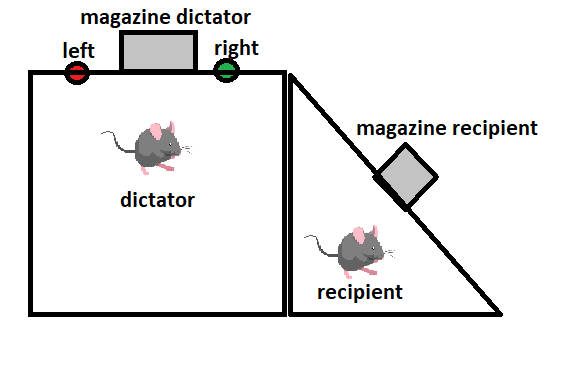
\includegraphics[scale=0.55]{altruism.png} 
	\end{center} 
	\caption{\textit{Main setting of the altruism task: a dictator mouse (left) can choose between two pokes, one of which will deliver a food pellet to a recipient mouse (right).}} \label{altruism}
	
\end{figure}

The \textit{altruism task} is a task in which two mice are tested in their social decision making. It consists in two mice located in adjacent compartments, separated by a metal mesh which allows them to see and sniff each other, but not enter in direct contact (Figure \ref{altruism}). One mouse, called the \textit{recipient}, assumes only a passive role: it stays in its space and, when a food delivery happens from an apposite box (called \textit{magazine}) it can eat the delivered food pellet. 
In contrast, the other mouse, called \textit{dictator}, has to perform a social choice. Indeed, in any case a food delivery to its own magazine will happen by poking one of two buttons available, but even if both types of pokes will provoke a pellet delivery for the dictator, only one of them will give food to the recipient as well. It follows that the two choices of the dictator can be classified as \textit{selfish} and \textit{altruistic} decisions.\\
In order to stimulate the seeking for food, mice have been kept at $ 90 \%$ of their standard body weight before the test. The setup is organized as follows:

\begin{itemize}
	
	\item Before the tasks were performed, both mice were kept together in same sex pairs for two weeks 
	
	\item The animals were tested for $5$ days. The first day involves a \textit{learning} process for the dictator to understand the food delivery mechanism. The main test is considered to be during the following $3$ days, and finally the process is considered well assimilated by the dictator during the final day	
	
	\item The position of the altruistic and selfish pokes (i.e. of the two buttons providing or not the food delivery to the recipient) has been randomized through the different days of the test, in order to rule out spatial causes for the results
	
	\item A control test has been performed in parallel. Here, the recipient mice were replaced by inanimate objects, in order to determine the effective relevance of their presence in the task
	
	\item During the performance of the $5$ days of the test, the calcium activity in the basolateral amygdala of the dictator has been recorded using the Fiberphotometry technique, giving as result a collective signal of the BLA activity (as discussed in Section \ref{section 1.4})
	
\end{itemize}



\section{Behavioural results in the altruism task}


\begin{figure}[H]
	\begin{minipage}{\linewidth}
		\centering
		\begin{minipage}{0.46\linewidth}
			\begin{figure}[H]
				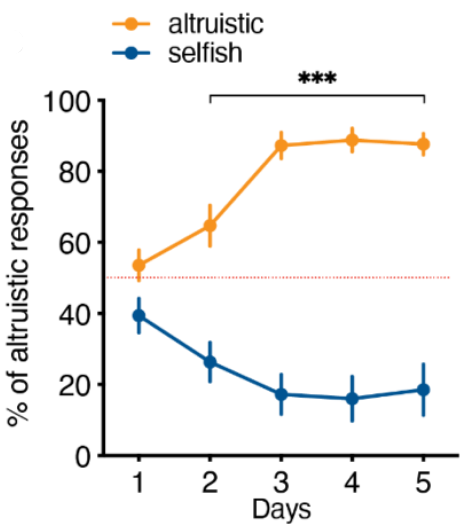
\includegraphics[width=\linewidth]{altr_self.png}
				
			\end{figure}
		\end{minipage}
		\hspace{0.05\linewidth}
		\begin{minipage}{0.46\linewidth}
			\begin{figure}[H]
				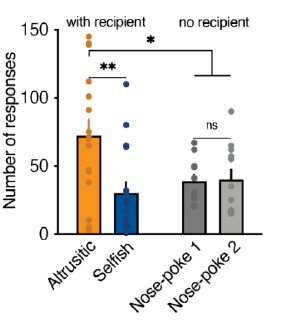
\includegraphics[width=\linewidth]{norecip.png}
				
			\end{figure}
		\end{minipage}
		
	\end{minipage}
	\caption{\textit{Left: Percentage of change in altruistic response (i.e in the number of altruistic pokes) for altruistic and selfish mice. Right: difference in number of altruistic and selfish pokes by the dictator when the recipient is present or not}} \label{altr_first}
\end{figure}



As shown in Figure \ref{altr_first}, the first evident result of the altruism task is that, when a recipient mouse was present and same sex pairs adopted, the dictator mice showed an increase in the number of altruistic pokes during the test days. In contrast, when recipient mice were replaced by inanimate objects, no appreciable difference between altruistic and selfish preferences have been detected. Such differences started to emerge from the second day of the test, as confirmation of a successful learning period on the first day. \\
An important difference has been observed between male and female mice:  only male dictators showed altruism preference, while female ones did not show an appreciable difference between selfish and altruistic pokes.\\
Next, the spatial exploration of the mice has been under investigation. Results indicate that altruistic dictators (i.e.dictators which showed preference for altruistic pokes) tend to explore more the area in proximity to the recipient, in contrast with selfish dictators which did not show particular interest in their partners.\\
To test whether visual interaction plays a role determining the altruistic preferences, the task has been repeated replacing the metal mesh with an opaque screen, which still allowed olfactory and auditory stimuli, but not visual ones. In this situation, mice showed a marked decrease in the altruistic responses, with respect to the previous case in which a metal mesh was used. This implies that the dictator mouse needs to be able to see the recipient partner getting the food delivery, in order to be able to select the altruistic alternative.\\
Finally, to further determine the ability of the dictator mice to \textit{learn} from experience and change their habits in light of an altruistic choice, dictators were tested with no partner in the adjacent cage, to trigger one nose poke over the other. Subsequently, the recipient mouse was put in the near cage, and the location of the altruistic poke, delivering food to it as well, has been assigned to the poke less pressed by the dictator. Despite this, the dictator showed through days a change in its preference towards the altruistic poke. Changing the recipient with an inanimate object, such preference decreased once again. The conclusion is straightforward: the presence of the recipient is the determining factor for the altruistic preference by the dictator.
\\

Once, in normal conditions, the altruistic preference has been established, one may ask under which conditions such preference is maintained. To this purpose, the task was repeated changing the rules of food delivering. Now, two nose pokes were necessary for the food delivery in the altruistic poke, while only one in the selfish one. Even with this additional effort, male and female mice which previously showed altruistic preferences, increased the number of altruistic over selfish preferences also in this case. Increasing the necessary number of pokes to $4$, male dictators kept their altruistic preferences, while female dictators did not show anymore a significant difference. Finally, requiring $6$ nose-pokes for altruistic delivery still kept male mice in their altruistic preference, while made female ones prefer the selfish one, and only from $8$ pokes, also males stopped to be altruistic. Overall, these results showed that \textit{male mice tend to share food with their cagemates partners, even at costly conditions} (Figure \ref{number_pokes}).\\
Finally, mice were tested in two more conditions: absence of rewards for both dictator and recipient mouse, and absence of reward for dictator, but not for the recipient mouse. While, in the first case, no preference between the two pokes was expressed by the dictator, in the second case there was an altruistic preference. This means that the dictator can choose an altruistic decision even if there is no direct benefit for itself.


\begin{figure}[H]
	\begin{center}
		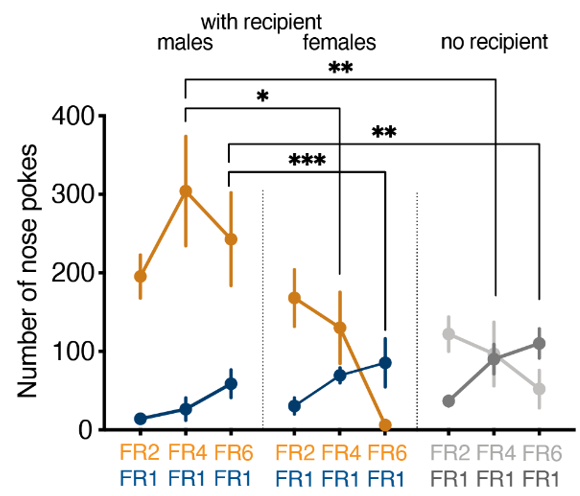
\includegraphics[scale=0.55]{number_pokes.png} 
	\end{center} 
	\caption{\textit{Number of nose pokes of male and female mice, with and without recipients, changing the number of nose-pokes necessary for a food delivery.}} \label{number_pokes}
	
\end{figure}

\section{The role of social hierarchy in altruism display}

\begin{figure}[H]
	\begin{center}
		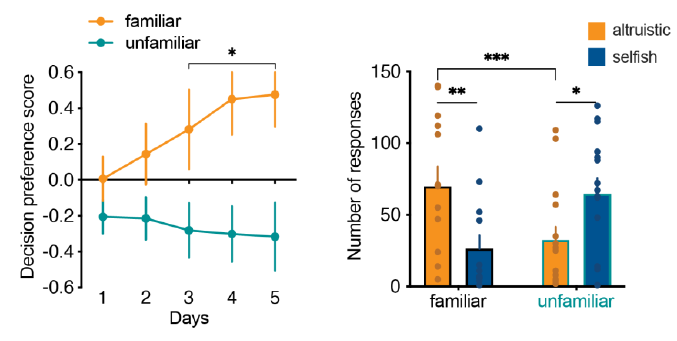
\includegraphics[scale=0.5]{familiar.png} 
	\end{center} 
	\caption{\textit{Left: decision preference score with familiar and unfamiliar recipients. Right: Number of responses by selfish and altruistic dictators, with familiar and unfamiliar recipients.}} \label{familiar}
	
\end{figure}

As of today, it has been recognized that familiarity between individuals plays a key role in social relationships \cite{31}. % [De Waal, F. B. M. \& Preston].
 In the case of the altruism task, it is to be expected that the altruism shown by the dictator is strictly depending on the period preceding the test, in which dictator and recipient have been cagemates for two weeks. To test this hypothesis, the task has been repeated using unfamiliar recipients, showing no preference for altruistic choices, where indeed most of dictator mice showed preference for the seflish pokes (Figure \ref{familiar}). This has been measured through the \textbf{decision preference score} 

\begin{equation}
DPS = \frac{A -S}{A+S}
\end{equation}

where $A$ and $S$ are the number of altruistic and selfish responses, respectively.\\
Next, a \textit{dominant/follower} relationship has been established through the \textbf{tube test}, in which two mice have been paired in a tube allowing the passage of just one individual. This test helped to figure out whice of the two was the \textit{dominant} individual, i.e. the one pushing the other, and the \textit{follower} individual, i.e. the one retreating. The dominance has been quantified through the \textbf{Normalized David's score} \cite{32} % [De Vries, H., Stevens, J. M. G. \& Vervaecke]

\begin{equation}
NDS = \frac{1}{N}\left(DS + \frac{N(N-1)}{2}\right)
\end{equation}

where $N$ is the number of tested subjects and $DS$ is the David's score, i.e. the ratio of wins.\\
The analysis of 9 pairs of mice ($N=18$) yielded the main following results:

\begin{enumerate}
	\item The dominance relationship is \textit{transitive}: if mouse A is dominant with respect to mouse B, and mouse B is dominant with respect to mouse C, then mouse A dominates also mouse C 
	
	\item Dictator mice showing selfish preferences in the altruism task displayed low scores in the $NDS$ compared to their recipients, which means that selfish dictators  tend to be less dominant than their corresponding recipients
	
	\item No significant differences have been detected between the dominance scores of altruistic dictators and their recipients
	
	\item The more a dictator has a higher dominance value $NDS$, the more it is willing to perform altruistic preferences in the altruism task
	
\end{enumerate}

Next, the study tested the hypothesis that \textit{an increase in altruism is related to an increase in affective state matching between individuals}. To do so, the recipient has been subject to a manipulation of its emotional state, in this case a fear conditioning paradigm through mild shocks. In the meantime, the dictator mouse (here assuming the role of \textit{observer}) was allowed to see the recipient through a transparent separating wall.\\
The main result was that altruistic mice displayed an increased freezing behaviour during this phase, compared to selfish ones. Since these latter are the dominant ones, this result leads to the conclusion that \textit{dominant mice tend to show more empathic-like behaviours}, from altruism to emotional contagion.

\section{Analysis of calcium activity in the BLA} \label{section 4.5}

\begin{figure}[H]
	\begin{center}
		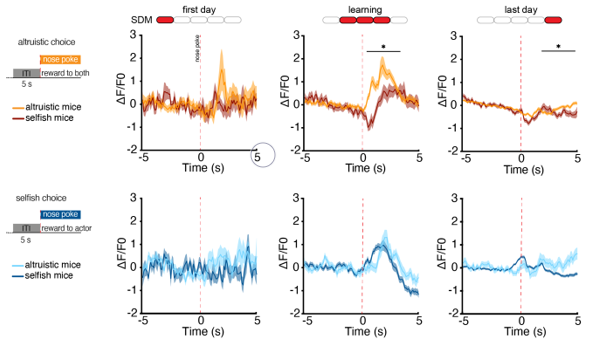
\includegraphics[scale=0.55]{psth.png} 
	\end{center} 
	\caption{\textit{Top row: PSTH of selfish and altruistic mice during nose pokes in altruistic pokes. Bottom row:  PSTH of selfish and altruistic mice during nose pokes in selfish pokes. Results have been averaged on all nose pokes.}}
	\label{psth}
\end{figure}

The Fiberphotometry analysis of the calcium activity in the BLA allowed us to establish a connection between the type of choice adopted by dictator mice and their corresponding neural activity. In order to analyze the relative change of such activities during altruistic or selfish pokes, the raw data from the photometry have been subjected to a \textbf{peristimulus time histogram (PSTH)} analysis. Such analysis goes through the following steps:

\begin{enumerate}
	
	\item Set a START and STOP time for the analysis, i.e. set the time window in which considering the variation of the neural activity (in this case START = STOP = $5$ $s$ for a window of $10$ $s$)
	
	\item For every time point $t$, presenting an activity given by Fiberphotometry $x_t$, consider the interval $[t-START , t+STOP]$
	
	\item Compute the mean $ \mu_t$ and standard deviation $\sigma_t$ of the activity in such interval
	
	\item The value of the PSTH for the selected time point is then
	$$ P_t = \frac{x_t - \mu_t}{\sigma_t}$$
\end{enumerate}
Next, in order to quantify the intensity of the activity, \textbf{areas under the curve (AUC)} were estimated numerically using the trapezoid quadrature rule [Quarteroni-Sacco].\\

The overall analysis on raw photometry data, PSTH tracks and AUC showed some remarkable results (Figure \ref{psth}):

\begin{itemize}
	
	\item Dictator mice showed an increased activity in the BLA when a recipient mouse was present, compared to the case where an inanimate object was placed in the near cage
	
	\item During the first and last day, in all cases no significant differences emerged in the activation of BLA
	
	\item In the intermediate days of learning, however, altruistic mice showed a strong activation during the nose poking in the altruistic pokes, but not in the selfish ones. Selfish mice, in contrast, did not show any particular activation of their neural activity during both pokes
	
	\item The AUC analysis suggested that the levels of activity were higher during the intermediate days, rather than in the first and last day
\end{itemize}


To further inspect the role of BLA neurons in empathy display, such neurons have been silenced via a \textbf{chemogenetic procedure} \cite{33}. % [Qi-Gang Zhou, Ashley D Nemes]. 
In this approach, a viral vector, carrying specific receptors, is injected into the area of interest. Such receptors, called  \textbf{hM4D receptors}, belong to the group of \textit{inhibitory designer receptors exclusively activated by designer drugs (DREADD)}, which activate themselves only when in contact with a particular drug, the \textbf{Clozapine N-oxide (CNO)}. In this way, mice injected with hM4D-CNO will exhibit an \textit{inhibition} of BLA-neurons. In contrast a control group of mice was injected with CNO only, without hM4D receptors.\\
The obtained results after these injections, displayed in Figure \ref{silencing}, showed a significant reduction of freezing behaviour in the dictators, while their recipient partners were subject to emotion conditioning as previously described. This confirms the conclusions of previous studies \cite{34}, % [Allsop, S. A. et al],
 namely a \textit{critical role of the amygdala in emotional matching}. Silencing BLA neurons revealed to be correlated also to the amount of altruism preferences. Indeed, mice with silenced BLA neurons failed to show a marked preference for altruistic choices, in contrast with the control case. Indeed, while approximately $3$ out of $4$ mice showed altruistic preferences in control conditions, a similar percentage of BLA-silenced mice showed preference for selfish pokes.\\
BLA silencing did not affect the number of responses or the latency of choices, rather it affected the type of the social decision. This is a further evidence of the primary role of BLA in altruism display.
\\
Finally,  silencing of BLA neurons appeared to reduce also the dominance (Figure \ref{sil_dom}): a higher number of BLA-silenced mice assumed a subordinate role with respect to control mice. In particular, if transitive relationships of dominance are distributed in levels $ \alpha \rightarrow \beta \rightarrow \gamma \rightarrow \delta $, silenced mice belong only to levels $ \gamma $ and $ \delta $.

\begin{figure}[H]
	\begin{center}
		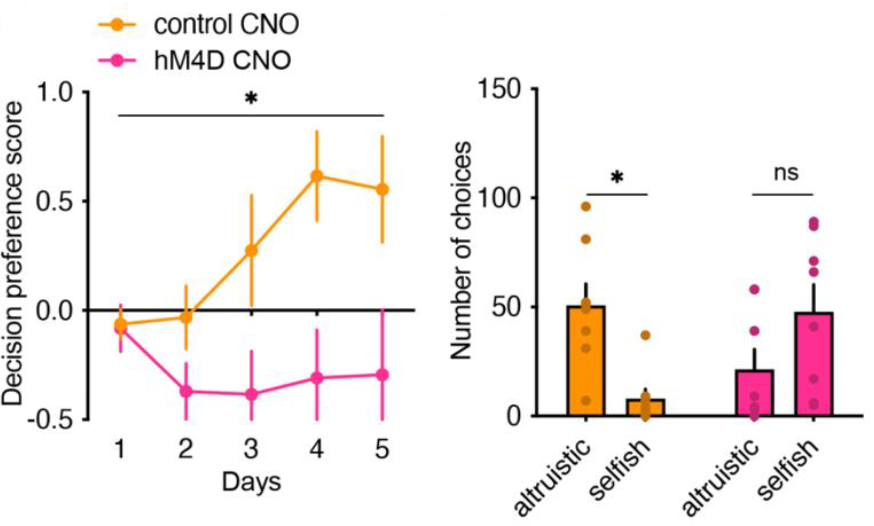
\includegraphics[scale=0.6]{silencing.png} 
	\end{center} 
	\caption{\textit{Left: Decision preference score in BLA-silenced mice (hM4D CNO) and non-silenced mice (control CNO). Right: number of selfish and altruistic pokes in BLA-silenced mice (hM4D CNO) and non-silenced mice (control CNO). }} \label{silencing}
	
\end{figure}


\begin{figure}[H]
	\begin{center}
		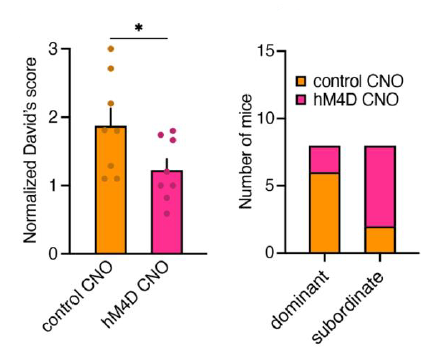
\includegraphics[scale=0.6]{sil_dom.png} 
	\end{center} 
	\caption{\textit{Left: Normalized David's score in BLA-silenced mice (hM4D CNO) and non-silenced mice (control CNO). Right: number of dominant and subordinate mice in BLA-silenced mice (hM4D CNO) and non-silenced mice (control CNO). }} \label{sil_dom}
	
\end{figure}

\newpage

\chapter{Mathematical modeling in cellular electrophysiology}

In Section \ref{first section}, the concept of \textit{excitability} of neurons has been introduced: neurons are able to generate and transmit \textbf{electrical impulses} as a response to external stimuli. These impulses are a direct consequence of rapid changes in intracellular end extracellular \textit{ionic concentrations} of main chemicals such as $Na^+, Cl^-, K^+, Ca^{2+}$. The change of such concentration values determines a change in the electric potential difference formed across the cell's membrane, and thus the formation of an \textbf{action potential}. \\
In this chapter, mathematical models to describe cellular electric activity are presented. After introducing the main assumptions of the models, the equivalent electric circuit formulations for cellular electrophyioslogy will be presented, along with different ways to describe its electrical components. Finally, the main model to describe the propagation of the action potential between two neurons will be considered, namely the \textbf{cable equation model}. All these models consist in either \textbf{ordinary differential equations (ODEs)} or \textbf{partial differential equations (PDEs)}, to be numerically solved through appropriate techniques, briefly discussed in the final part of the chapter.

\section{Electric activity in neurons}


\begin{figure}[H]
	\begin{center}
		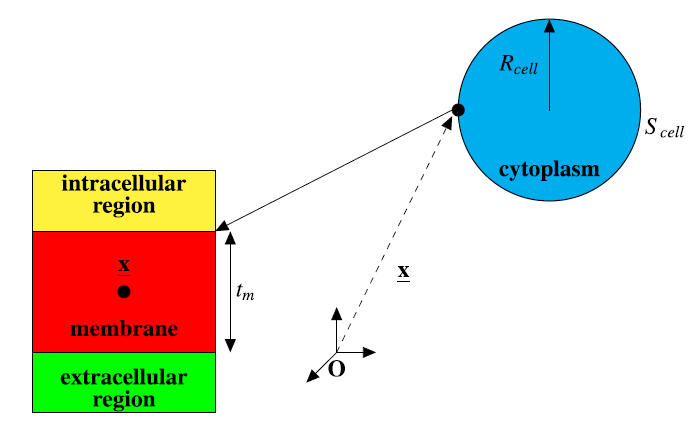
\includegraphics[scale=0.7]{first.png} 
	\end{center} 
	\caption{\textit{Schematic model of a cell with a focus on a local point $\textbf{x}$ of the membrane.}}
	\label{first}
\end{figure}




In order to mathematically describe the main electric functionalities of a cell, we first need to understand the set of phenomena which characterize this complex component of our body, such as the processes leading to its condition of \textit{dynamical equilibirium}, called the \textbf{cellular homeostasis}. The cellular homeostasis is achieved through the equilibrium of several forces acting on the cell, which can be of fluid, mechanical, chemical or electric nature, although the focus in this work will regard only the elctrical part.\\
The \textit{intracellular} environment of a cell consists mainly in a water solution contaning vital nutrients and elements in ionic form such as  $Na^+, Cl^-, K^+, Ca^{2+}$, making the solution behaving like a charged fluid. The intracellular environment is separated by the extracellular one by the \textbf{membrane} of the cell (see Figure \ref{first}). The membrane, schematized in Figure \ref{membrane scheme}, is formed by a bilayer of lipids (of thickness considerably smaller than the cell's radius) which does not allow passage of substances through it. The passage of some ions is still allowed through specific sites called \textbf{ionic channels}, each of one allowing, under certain conditions, the passage of a single ionic species. The movement of one ionic species from the intracellular to the extracellular environment, or viceversa, is caused by the different concentration of such quantity in the two regions, leading to an \textit{electrochemical gradient} which forces positive charges to move from high to low potentials, and thus forming a potential difference across the membrane. We call this quantity the \textbf{membrane potential} of the cell. The main role of the mathematical models for cellular electrophysiology is to describe the evolution of such quantity over time and space.
\\
\begin{figure}[H]
	
	
	\centering
	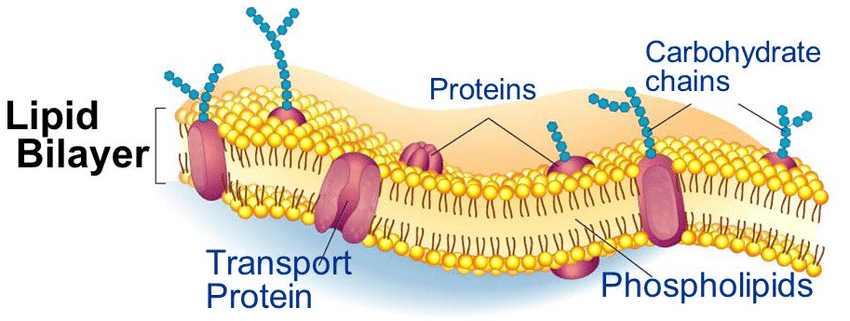
\includegraphics[scale=0.55]{membrane.png}
	
	
	
	\caption{\textit {Schematic representation of the cellular membrane.}} \label{membrane scheme}
	
\end{figure}
The particular biology of the cell makes it at the same time a \textit{dielectric} and a \textit{conductor}: the lipid layers of the membrane isolate the intracellular environment from the external environment, and cause the accumulation of charges of opposite sign around the internal and external surfaces of the membrane. This effect is typical of dielectric materials such as capacitors, and it will cause a \textit{capacitive} current across the membrane. This current is not associated with motion of ions, but to the time rate of change of the surface charge on each side of the membrane. On the other side, when an ionic channel is open, there is a passage of ions which makes the cell behaving like a conductor. Both of these contributes need to be taken into account in the modeling of the cell, as done in the next Section.
\\

In order to start modeling these electrical phenomena, let us consider a geometrical setting representing the relevant components of a cell in its electrical activity, with the following assumptions:

\begin{enumerate}
	
	\item The cell is modeled as a sphere of radius $R_c$ and surface $ S_c = 4\pi R_c^2$
	
	\item The intracellular environment $\Omega_{in}$ is separated by the extracellular region $\Omega_{out}$ by the membrane, with internal surface $\Sigma_{in}$ and external surface $\Sigma_{out}$.% Define the outward unit normal vectors to these surfaces as $\textbf{n}_{in}$  and  $\textbf{n}_{out} = - \textbf{n}_{in}$
	
	\item The thickness of the membrane $t_m$ is such that $ \eta_c := \frac{t_m}{R_c} << 1$. This allow us to neglect it and assume that $\Sigma_{in} \sim \Sigma_{out} \sim \Sigma$ \label{ass 3}
	
	\item The dielectric behaviour of the membrane is expressed by a \textbf{membrane capacitance}  $ c_m = \frac{\varepsilon_m}{t_m} $, where $\varepsilon_m$ is the dielectric constant of the membrane \label{ass 4}
	
\end{enumerate}

Let us consider now two points $ \textbf{x}' \in \Sigma_{in}$ and $ \textbf{x}'' \in \Sigma_{out}$, as represented in Figure \ref{intra}. The axis connecting $ \textbf{x}'$ and $ \textbf{x}''$ is denoted by $x$ and $\textbf{e}$ is the unit vector oriented from $\Omega_{in}$ to $\Omega_{out}$. For any time $ t \in [0,T]$, we introduce the electric potentials $ \psi^{in} (\textbf{x}',t) $ and  $ \psi^{out} (\textbf{x}'',t) $. The \textbf{membrane potential} at $ \textbf{x} \in \Sigma$ is 

\begin{equation}
\psi_m (\textbf{x},t) = \psi^{in} (\textbf{x}',t) -  \psi^{out} (\textbf{x}'',t) \hspace{0.5 cm}  t \in [0,T], \hspace{0.5 cm} \textbf{x} \in \Sigma
\end{equation}


\begin{figure}[H]	
	
	\centering
	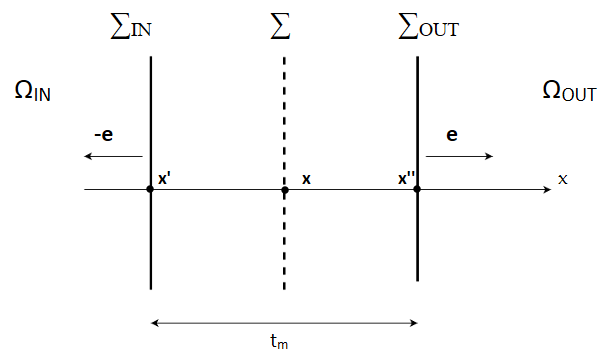
\includegraphics[scale=0.65]{intra.png}
	
	\caption{\textit {Mathematical representation of the cellular membrane.}} \label{intra}
	
\end{figure}

Having introduced the above geometrical description of the cell's membrane, we define the \textbf{total current density}  as

\begin{equation}
\textbf{e} J^{TOT}(\textbf{x},t) =	\textbf{J}^{TOT}(\textbf{x},t) = \textbf{J}^{cond}_{TOT}(\textbf{x},t) +\textbf{J}^{cap}(\textbf{x},t) 
\end{equation}	

which consists in the following two contributions:

\begin{itemize}
	
	\item \textbf{Conduction current density}: 
	\begin{equation}
	\textbf{J}^{cond}_{TOT}(\textbf{x},t) = \sum_{\alpha} \textbf{J}_{\alpha}(\textbf{x},t)
	\end{equation}
	where $\textbf{J}_{\alpha}(\textbf{x},t) = \textbf{e} J_{\alpha}(\textbf{x},t)$ is the current associated with the conduction of ion species $\alpha$ along the ionic channel.
	
	\item \textbf{Capacitive current} 
	
	\begin{align}
	\textbf{J}^{cap}(\textbf{x},t) &= \frac{\partial \textbf{D}(\textbf{x},t)}{\partial t}\\	
	\textbf{D}(\textbf{x},t) &= \varepsilon_m \textbf{E}(\textbf{x},t)
	\end{align}
	
	
	
	
	where $\textbf{D}(\textbf{x},t)$ is the electric displacement vector at $\textbf{x}$ $\forall t \in [0,T]$ and $\textbf{E}(\textbf{x},t)$ is the electric field. Assuming quasi-static conditions we have
	
	\begin{equation}
	\textbf{E}(\textbf{x},t) = - \nabla \psi(\textbf{x},t)
	\end{equation}
	
	so that
	
	\begin{equation}
	\textbf{J}^{cap}(\textbf{x},t) = -\varepsilon_m \frac{\partial}{\partial t}\nabla \psi(\textbf{x},t)
	\end{equation}
	
	
	
	Using assumption (\ref{ass 3}), we may write 
	
	$$ - \nabla \psi(\textbf{x},t) \simeq - \textbf{e} \frac{\psi(\textbf{x}'',t) - \psi(\textbf{x}',t)}{t_m} = \textbf{e} \frac{\psi_m(\textbf{x},t) }{t_m} $$
	
	Finally, using assumption (\ref{ass 4}), the capacitive current density takes the form
	\begin{equation}
	\textbf{J}^{cap}(\textbf{x},t) = \textbf{e} c_m \frac{\partial \psi_m (\textbf{x},t)}{\partial t}
	\end{equation}
\end{itemize}	

In conclusion, the total current density flowing across the cell membrane at $ \textbf{x} \in \Sigma$ $\forall t \in [0,T]$ is given by

\begin{equation}
\textbf{J}^{TOT}(\textbf{x},t) = \sum_{\alpha} \textbf{e} J_{\alpha}(\textbf{x},t) + \textbf{e} c_m \frac{\partial \psi_m (\textbf{x},t)}{\partial t} \label{Jtot}
\end{equation}

In the next sections, we are going to use Eq. (\ref{Jtot}) in the construction of local and global models for the electric activity of the cell. While the quantity $c_m$ is typical of the cell and taken from experimental observations, the modeling will involve the conduction current. 

\begin{remark}
	The quantity $\textbf{J}^{cap}$ is defined to as capacitive current density because it mathematically represents the effect of the time rate of change of the surface charge density 
	
	$$ \sigma(\textbf{x},t) = c_m \psi_m (\textbf{x},t) = c_m \left(\psi(\textbf{x}',t) - \psi(\textbf{x}'',t) \right)$$
	which accumulates with opposite sign on the internal ($\sigma_{in}$) and external ($\sigma_{out}$) surfaces $\Sigma_{in}$ and $\Sigma_{out}$ in such a way that
	
	$$ \sigma_{in} = -\sigma_{out} $$
	
	According to this interpretation, the cell membrane, in the neighbourhood of $ \textbf{x} \in \Sigma$, can be regarded as a capacitor with plane plates separated by a dielectric medium (the lipid bilayer) with specific capacitance $ c_m = \frac{\varepsilon_m}{t_m}$ and surface charge density $\sigma(\textbf{x},t)$.
\end{remark}












\begin{table}[H]
	\begin{center}
		\begin{tabular}{ |c|c|c|c| } 
			\hline
			\textbf{Electric quantity} & \textbf{Name} & \textbf{Unit measure} \\
			\hline
			$t_m$ & Membrane thickness & $m$ \\ 
			\hline
			$R_c$ & Cell radius & $m$ \\
			\hline
			$\psi_m$ & Membrane potential & $V$ \\
			\hline
			$J$ & Current density & $A/m^2$ \\
			\hline
			$I$ & Current & $A$ \\
			\hline
			$\sigma$ & Surface charge density & $C/m^2$ \\
			\hline
			$c_m$ & Specific membrane capacitance & $F/m^2$ \\
			\hline
			$C_m$ & Membrane capacitance & $F$ \\
			\hline
			$g_m$ & Specific membrane conductance & $S/m^2$ \\
			\hline
			$G_m$ & Membrane conductance & $S$ \\
			
			\hline
		\end{tabular}
		
	\end{center}
	\caption{\textit{Main electrical quantities in cellular electrophysiology.}}
\end{table}


\section{ODE local and global models}

\begin{figure}[H]
	
		
	
			\begin{figure}[H]
				\centering
				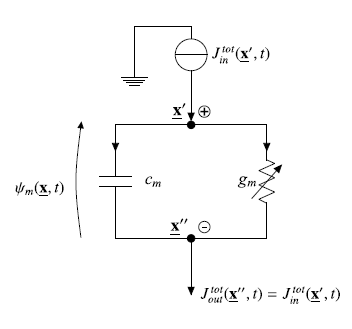
\includegraphics[scale=0.6]{ode_circuit.png}
				
			\end{figure}
		
	\caption{\textit{Equivalent circuit for a fixed point $\textbf{x} \in \Sigma$ (local model).
		}} \label{circuit}
\end{figure}


Considering  a point $\textbf{x} \in \Sigma$, equation (\ref{Jtot}) expresses a balance law for the current densities $J^{TOT}$, which can be divided in two contributions (capactive and conduction), where the capacitive current assumes the form $$J^{cap}(\textbf{x},t) = c_m \frac{\partial \psi_m(\textbf{x},t)}{\partial t}$$
The conduction current takes the general form 

\begin{equation}
J^{cond}_{\alpha}(\textbf{x},t) = g_m(\textbf{x},t,\psi_m(\textbf{x},t)) [\psi_m(\textbf{x},t) - E_{c,\alpha}] \label{conduction current}
\end{equation}

where $g_m$ is the \textbf{specific conductance}, depending on $\psi_m$, and $E_{c,\alpha}$ is the \textbf{Nernst potential}, which corresponds to the  membrane potential for which the ion conduction current is equal to $0$.\\
The two above expressions for the current densities can be syntethized in a \textit{circuital form}, in which their two contributions (capacitive and conduction) are modeled respectively through a specific capacitance and a specific conductance (see Figure \ref{circuit}). Then, an application of the Kirchhoff current law  gives the current balance for the circuit.\\
For any fixed $\textbf{x} \in \Sigma$,  equation (\ref{Jtot}) is an \textbf{ordinary differential equation (ODE)} in the unknown $\psi_m$. This model is a \textit{local} model, since the focus has been on a specific point of the membrane $\textbf{x}$.
\\
If instead of a specific $\textbf{x} \in \Sigma$, the aim is to write a current balance across the whole cell's membrane $\Sigma$, the resulting differential equation, which in this case expresses a \textit{global} whole cell model, is obtained by integration of (\ref{Jtot})  over the surface $\Sigma$,  which yields the conservation of the total current 

\begin{equation}
I_{\alpha}^{TOT} = \int_{\Sigma} \textbf{J}_{\alpha}^{TOT} \cdot \textbf{n}_{out} dS 
\end{equation} 
In this case, we need to define the whole cell membane conductance $ G_m$ and capacitance $ C_m $, so that the current balance takes the form

\begin{equation}
I_{\alpha}^{TOT}(t) = I_{\alpha}^{cap}(t) + I_{\alpha}^{cond}(t)
\end{equation}

where $  I_{\alpha}^{cap}(t) = C_m \frac{d \psi_m(t)}{d t}$ and $ I_{\alpha}^{cond}(t) = G_m(t,\psi_m) [\psi_m(t) - E_{c,\alpha}]$.\\
While the (specific) capacitance is an intrinsic value of the cell, the conduction current, and  in particular the (specific) conductance $G_m$, need to be modeled. In the next sections, three main models used in literature for this purpose will be presented: the \textbf{linear resistor model (LRM)}, the \textbf{Goldman-Hodgkin-Katz (GHK)} model and finally the \textbf{Hodgkin-Huxley (HH)} model.\\




\section{The Linear Resistor Model (LRM)}

\begin{figure}[H]
	\begin{center}
		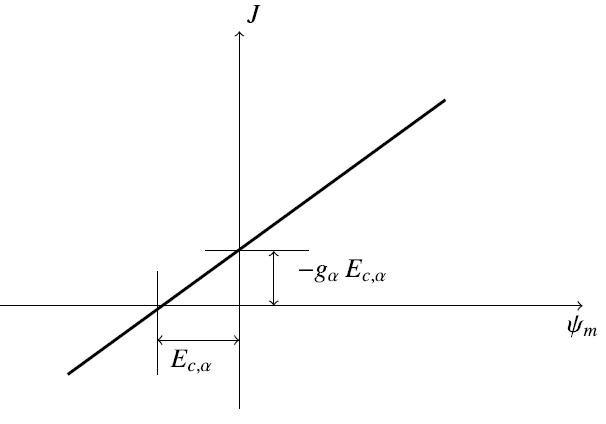
\includegraphics[scale=0.65]{LRM.png} 
	\end{center} 
	\caption{\textit{Characteristic curve for the linear resistor model.}} \label{LRM}
	
\end{figure}

The \textbf{linear resistor model (LRM)} makes the simplest assumptions 

\begin{equation}
g_{m,\alpha}(\textbf{x},t,\psi_m(\textbf{x},t)) = g_{m,\alpha}^0 = const \hspace{1.5 cm} E_{c,\alpha}(\textbf{x},t) := E_{c,\alpha}^0 = const \hspace{1cm} \forall \alpha
\end{equation}

Therefore, this model assumes the conductance and the Nernst potential as constant.
The resulting expression for the conduction current density is
\begin{equation}
J_G(t) = g_{m,\alpha}^0 [\psi_m -  E_{c,\alpha}^0]
\end{equation}

This law defines a straight line in the plane $J_G$ vs $\psi_m$ (Figure \ref{LRM}), such that there exists a unique value of membrane potential for which $J_G=0$. This value is exactly the Nernst potential $E_{c,\alpha}^0$ .


The Nernst potential $E_{c,\alpha}^0$is related to the concept of  \textbf{thermodynamic equilibrium}. Micorscopic theory assumes that ion particles in the channel are subjected to two different contributions: diffusion process caused by the chemical gradient, and a transport caused by the presence of an \textit{electrical field} $\textbf{E}(\textbf{x},t)$ \cite{35}.% [Sacco-Guidoboni].
 This phenomenological perspective leads to the \textbf{drift-diffusion (DD)} model for the conduction current density, which reads

\begin{equation}
\textbf{J}_{\alpha}^{DD} = \textbf{J}_{\alpha}^{DIFF} + \textbf{J}_{\alpha}^{DRIFT} = -Fz_{\alpha}D_{\alpha}\nabla C_{\alpha} + F|z_{\alpha}| C_{\alpha}\mu_{\alpha}\textbf{E}
\label{DD}
\end{equation}
where 
\begin{itemize}
	
	\item $F$ is the \textbf{Faraday constant}, such that $F = q N_{av}$, being $q$ the elementary charge and $N_{av}$ the Avogadro's constant
	
	\item $z_{\alpha}$ is the \textbf{ion number}, positive for cations and negative for anions
	
	\item $\mu_{\alpha}$ is the \textbf{ion electrical mobility}
	
	\item $C_{\alpha}$ is the molar density of ion $\alpha$
	
	\item $D_{\alpha}$ is the \textbf{ion diffusivity}. this value can be retrieved from the \textit{Einstein-Smoluchowki} relation \cite{36} %[Md. Akhtarul Islam]
	 $D_{\alpha} = V_{TH}\frac{\mu_{\alpha}}{|z_{\alpha}|}$, where $ V_{TH} \sim 26$ $mV$ is the \textit{thermal voltage}
\end{itemize}

\begin{theorem}
	Let us assume a one dimensional gemetry as in Figure \ref{intra}. Then, the thermodynamic equilibrium, for which $\textbf{J}_{\alpha}^{DD} = 0$ and  the drift current density balances the diffusion current density, is obtained in correspondence of the value of the membrane potential
	
	\begin{equation}
	E_{c,\alpha}^0 = \frac{V_{TH}}{z_{\alpha}}\ln\left(\frac{C_{\alpha}^{OUT}}{C_{\alpha}^{IN}}\right)
	\end{equation}	
	
	
\end{theorem}




\section{The Goldman-Hodgkin-Katz model (GHK)}
With the \textbf{Goldman-Hodgkin-Katz (GHK)} model, the modeling of the conduction current becomes nonlinear. Here, the following assumptions are adopted: 

\begin{itemize}
	
	\item The electric field in the ionic channel assumes a constant value of $ E = \frac{\psi_m}{t_m}$, i.e. the ratio between the membrane potential and the membrane thickness
	
	\item The geometrical setting is one dimensional
	
	\item The conduction current $\textbf{J}_{\alpha}^{cond}$ varies only in time, i.e. is constant in space and $ \frac{\partial J_{\alpha}^{cond} }{\partial x} = 0$. This means that there is no production or consumtpion of ions along the channel
	
\end{itemize}

Applying these hypothesis to Eq. (\ref{DD}), it can be shown that the conduction current density takes the form

\begin{equation}
J_{\alpha}^{GHK}(\psi_m,t) = -qz_{\alpha}P_{\alpha}\left[n_{\alpha}^{out} \mathcal{B}(\beta_m) - n_{\alpha}^{in} \mathcal{B}(-\beta_m) \right] \label{GHK}
\end{equation}

where $P_{\alpha} = \frac{D_{\alpha}}{t_m}$ is the \textbf{membrane permeability}, $ \beta_m := \frac{z_{\alpha} \psi_m}{V_th}$ and $ \mathcal{B}(x) = \frac{x}{e^x -1}$ is the \textbf{inverse Bernoulli function}.\\
It can be proven \cite{35} that (\ref{GHK}) can be written in the general form (\ref{conduction current}) by setting:

\begin{equation}
g_{\alpha}(\psi_m,t) = P_{\alpha}\frac{q z_{\alpha}^2N_{av}C_{\alpha}^{in}(t)}{V_{TH}} 
\end{equation}

\begin{equation}
E_{c,\alpha}(\psi_m,t) = P_{\alpha}\frac{V_{TH}}{z_{\alpha}} \left(\frac{C_{\alpha}^{out}(t)}{C_{\alpha}^{in}(t)} - 1\right)\mathcal{B}(\beta_m)
\end{equation}



\section{The Hodgkin-Huxley model (HH)}

\begin{figure}[H]
	\begin{center}
		\includegraphics[scale=0.65]{HH.png} 
	\end{center} 
	\caption{\textit{Equivalent circuit for the Hodgkin-Huxley model}} \label{HH}
	
\end{figure}


In 1963, Hodgkin and Huxley (HH) published in a paper a revolutionary work, which awarded them the Nobel prize, on mathematical modeling of the electrophyisiogical activity of cells, with the focus on the neurons of the giant squid \cite{37}.  %[Hodgkin-Huxley]. 
The equivalent circuit of the HH model is shown in Figure \ref{HH}. The main assumptions of the model can be resumed as follows:

\begin{itemize}
	
	\item The total current density $J^{tot}$ can be split in two contributions: a capacitive transmembrane current $J_{cap}^{tm} = c_m \frac{\partial \psi_m}{\partial t}$, where the capacitance is assumed to be a constant quantity, and, for every ion considered, a conduction transmembrane current  $J_{cond}^{tm}$ to be modeled. The main ions considered are \textit{potassium} ($K^+$) and \textit{sodium} ($Na^+$). The remaining contribution is mostly due to \textit{chlorine} ($Cl^-$) and is summarized in a \textit{leakage} current $J_L^{tm}$
	
	\item With every ion $\alpha$ is associated its Nernst potential $E_{c,\alpha}$, representing the value for which thermodynamic equilibrium is achieved for each ion current density
	
	\item In order to better describe what happens at a biological level of the cell membrane, the ionic channel have a \textit{state}, i.e. an associated probability value which expresses the percentage of their opening. Indeed, the behaviour of ionic exchange between the cytoplasm and the extracellular environment, strongly depends on the closing and opening of the ionic channel. With the HH model, the attempt is to mathematrically describe the opening status of the channel along time
	
	
\end{itemize}	


In the original form of the paper, a change of variable is performed: let us define the equilibrium potential of the whole cell as $E_m$, and define for every ion $\alpha$ the quantities

\begin{equation}
v_\alpha := E_{c,\alpha} - E_m \hspace{2cm}  v := \psi_m - E_m
\end{equation}

In this way, the form of the current density of ion $\alpha$ becomes


\begin{equation}
J_\alpha^{cond} = g_{m,\alpha}(v-v_\alpha)
\end{equation}

and the Kirchhoff current law for the circuit, expressed for the new variable $v = v(t)$, is

\begin{equation}	
\begin{cases}
J^{tot} = \displaystyle c_m \frac{\partial v}{\partial t} + g_{Na}(v - v_{Na}) + g_{K}(v - v_{K}) +g_{L}(v - v_{L})  \\
v(0) = 0
\end{cases}	\end{equation}


having assumed the membrane potential at equilibrium at time $t=0$.\\
For the whole equilibrium potential $E_m$, the \textbf{Goldman potential} can be used \cite{38}% [Ermantraut-Terman]


\begin{equation}
E_m= V_{TH} \ln \left[\frac{P_{Na} C_{Na}^{out} + P_{K} C_K^{out} + P_{Cl} C_{Cl}^{in}}{P_{Na} C_{Na}^{in} + P_{K} C_K^{in} + P_{Cl} C_{Cl}^{out}}\right]
\end{equation}

where $P_\alpha$ and $C_\alpha$  denote the permeability and molar density of ion $\alpha$, respectively.\\
As for the modeling of conductances, let us introduce the \textbf{gating variables} $n,m,h$ for the three considered ion species $K^+,Na^-,Cl^-$. They represent the probability of opening of the ionic channel. For example, if the cell is in a situation in which $C_{Na}^{out} > C_{Na}^{in}$, the opening of $Na^+$ channel will result in a current flow from outside to inside, and to a corresponding rise of the potential $\psi_m$. When the membrane potential reaches the value of equilibrium $E_{Na}$, the sodium channel will close. For this reason, the gating variables are expressed as the solution of ordinary differential equation of the type

\begin{equation}
\frac{dy}{dt} = \gamma (1-y) - \delta y \hspace{1 cm} \gamma,\delta >0  \hspace{1 cm} y = m,n,h
\end{equation}

so that there is a balance between a production rate $\gamma$ and a consumption rate $\delta$. The solution of an ODE in this form is

\begin{equation}
y(t) = y_\infty \left[1 - \exp\left(\frac{-t}{\tau}\right)\right]
\end{equation}

where

\begin{equation}
y_\infty = \frac{\gamma}{\gamma + \delta} \hspace{1.5cm} \tau = \frac{1}{\gamma + \delta}
\end{equation}

For the potassium conductance, the chosen dependence on its gating variable (in agreement with experimental data) is $ g_K = \bar{g}_K n^4$. For the sodium variable, it has been observed that also a second process is involved, so that the proposed form is  $ g_{Na} = \bar{g}_{Na} m^3h$. The values $\bar{g}_K$ and $\bar{g}_{Na}$ are constant and determined to fitting of experimental data.\\
To summarize, the HH model consists in the following sytem of nonlinear ordinary differential equations:

\begin{equation} 
\begin{cases}
J^{tot} =  c_m \displaystyle \frac{d v}{d t} + J_{Na} + J_K +J_L  & \text{(Kirchoff current law)}\\
J_\alpha = g_\alpha (v-v_\alpha) \hspace{1 cm}  \alpha = Na,K,Cl & \text{(Conduction current densities)}\\
\displaystyle \frac{dn}{dt} = \gamma_n(1-n) -  \delta_n n & \text{(ODE for gating variable n)} \\[0.7em]
\displaystyle \frac{dm}{dt} =  \gamma_m(1-m) -  \delta_m m & \text{(ODE for gating variable m)}\\[0.7em]
\displaystyle \frac{dh}{dt} =  \gamma_h(1-h) -  \delta_h h & \text{(ODE for gating variable h)}\\ 
g_K = \bar{g}_K n^4 & \text{(Modeling conductance for K)}\\
g_{Na} = \bar{g}_{Na} m^3h  & \text{(Modeling conductance for Na)}

\end{cases}
\end{equation}

%\begin{figure}[H]
%	\begin{center}
%		\includegraphics[scale=1.4]{gk.png} 
%	\end{center} 
%	\caption{\textit{Example of behaviour of the potassium conductance $g_K$: a s%tep increase is followed by a decrease. The dots are experimental data}}
	
%\end{figure}


\section{The cable model} \label{section cable}

\begin{figure}[H]
	\begin{center}
		\hspace*{-0.7cm}
		\includegraphics[scale=0.63]{cable.png} 
	\end{center} 
	\caption{\textit{Schematic representation of the cable model.}}
	\label{cable}
\end{figure}


The models studied so far described the dynamic evolution of the membrane potential  for a single cell. In order to go further, we need to keep into account also the \textit{communication} between two cells, i.e. the propagation of the action potential from one neuron to another. Biologically, this propagation is mediated by the \textit{axon} connecting the two units. The axon is a part of the neuron, and at its every point we may assume a communication with the surrounding environment through electrical circuits as described in the previous sections.\\
The main assumptions for the cable model, schematized in Figure \ref{cable}, are the following:

\begin{itemize}
	
	\item The biological cable, i.e. the axon, has length $L$ and radius $a$ (thus a cross-sectional area  $S=\pi a^2$), with $\frac{a}{L} << 1$, allowing us to represent the cable as a $1D$ object along a longitudinal axis $ x \in [0,L]$
	
	\item The electric potential in the extracellular region is constant, as well as the intra and extra cellular concentration of every ion $\alpha$: 
	$$ \psi^{out}(x,t) = const  \hspace{1cm} C_\alpha^{in}(x,t)  = const \hspace{1cm} C_\alpha^{out}(x,t)  = const$$
	
	\item The \textbf{resistivity} of the axon $\rho_{ax}$ is constant. The resitivity is the reciprocal of the \textit{conductivity} $\sigma$, and is related to the \textit{resistance} $R_{ax}$ by
	 $$ R_{ax} = \frac{\rho_{ax} L}{S} $$
	
	
\end{itemize}


If we consider an element of length $dx$ of the cable, its contribution to resistance is $$dR(x) = \frac{\rho_{ax} dx}{\pi a^2}$$ If a current $I_{in}$ enters the element, the consequent potential difference across the element is 
$$ d\psi_m(x,t) = - \left(\psi_m(x+dx,t) - \psi_m(x,t)\right) = dR(x)I_{in}(x,t) = \frac{\rho_{ax} dx}{\pi a^2} I_{in}(x,t)$$ Therefore, letting $dx \rightarrow 0$, this implies that

\begin{equation}
I_{in}(x,t) = -\frac{\pi a^2}{\rho_{ax}}\frac{\partial \psi_m(x,t)}{\partial x}
\end{equation}

Next, to express a current balance at each point $x$, we need to consider again an infinitesimal element $dx$, in which a current $I_{in}(x,t)$ is entering the element, a current $I_{in}(x+dx,t)$ is leaving the element, and a transmembrane current $I_{TM}(x+\frac{dx}{2},t)$ is flowing from the axon to the extracellular environment, with a capacitive and a conduction contributions, as shown in Figure \ref{curr_bal}.\\
The application of Kirchhoff current law at the node  $x+\frac{dx}{2}$ gives

\begin{equation}
- I_{in}(x,t) + I_{cap}(x+\frac{dx}{2},t) + I_{cond}(x+\frac{dx}{2},t) + I_{in}(x+dx,t) = 0 \label{kirch}
\end{equation}

\begin{figure}[H]
	\begin{center}
		
		\includegraphics[scale=0.6]{curr_bal.png} 
	\end{center} 
	\caption{\textit{Current balance in an element $dx$ of the axon.}} \label{curr_bal}
	
\end{figure}

The capactive and conductive contributions to the transmembrane current are
\begin{equation}
I_{cap}(x+\frac{dx}{2},t) = J_{cap}(x+\frac{dx}{2},t) 2 \pi a dx = c_m \frac{\partial \psi_m(x,t)}{\partial t} 2 \pi a dx 
\end{equation}

\begin{equation}
I_{cond}(x+\frac{dx}{2},t) = J_{cond}(x+\frac{dx}{2},t) 2 \pi a dx 
\end{equation}

where $J_{cond}$ can be mathematically described using any of the LR, GHK or HH models. Dividing equation (\ref{kirch})  by $2 \pi a dx $ and letting $dx \rightarrow 0$ gives rise to the equation system

\begin{equation}
\begin{cases}
 \frac{ \displaystyle \partial \psi_m(x,t)}{\displaystyle \partial t} + \displaystyle \frac{\displaystyle 1}{ \displaystyle2 \pi a }\frac{\displaystyle \partial I_{in}(x,t)}{\displaystyle \partial x} + J_{cond}(x,t) = 0 \\[1em]
I_{in}(x,t) =   -\frac{\displaystyle \pi a^2}{\displaystyle \rho_{ax}}\frac{\displaystyle \partial \psi_m(x,t)}{\displaystyle \partial x}
\end{cases} \label{balance pde}
\end{equation}

The balance law (\ref{balance pde}) is a \textit{parabolic partial differential equation} for the unknown membrane potential $\psi_m(x,t) $, varying along space and time. To be solvable, (\ref*{balance pde}) needs to to be completed with an \textbf{initial condition} $ \psi_m (x,0) = \psi_m^0(x)$ and appropriate \textbf{boundary conditions}. The nature of the cable equation is linear or nonlinear depending on the chosen model for $J_{cond}$.\\
As for the boundary conditions, a common choice is to consider \textit{Dirichlet-Robin boundary conditions}. Defining the potential at $x=0$ as $\bar{V}_{in}(t)$ and modeling the right-hand terminal of the axon through a resistance $R_{out}$, the resulting boundary conditions are

\begin{equation}
\begin{cases}
\psi_m(0,t) = \bar{V}_{in}(t) \\
-I_{in}(L,t) +\displaystyle \frac{1}{R_{out}}\psi_m(L,t) =0
\end{cases}
\end{equation}



\section{Numerical solution of the cable equation}


\begin{figure}[H]
	\begin{center}
		
		\includegraphics[scale=0.7]{basis.png} 
	\end{center} 
	\caption{\textit{Lagrangian basis functions}}
	\label{Lagrangian}
\end{figure}


The cable equation model is an example of the following one-dimensional \textit{diffusion-reaction} boundary value problem for the unknowns $ u(x,t)$ and $\textbf{J} = J(x,t)\textbf{e}$:


\begin{equation}
\begin{cases}
\displaystyle \frac{\partial u}{\partial t} + \displaystyle \frac{\partial J}{\partial x} = \mathcal{P} & \forall (x,t) \in (0,L) \times (0,T)  \\[1em]
J = - \displaystyle \mu \frac{\partial u}{\partial x} & \forall (x,t) \in (0,L) \times (0,T)\\[1em]
u(x,0) = u^0(x) & \forall x \in (0,L)  \\
\gamma \textbf{J} \cdot \textbf{n} = \alpha u - \beta &  \forall (x,t) \in \partial \Omega \times (0,T)  
\end{cases} \label{dr}
\end{equation}

Here, $\textbf{J}$  represents a \textit{flux} taking into account the diffusion, while $\mathcal{P}$ takes into account the  net production rate. The boundary coefficients $\alpha, \beta, \gamma$ allow to recover the main types of boundary conditions (Dirichlet, Neumann, Robin).\\
In order to numerically solve the equation system (\ref{dr}), the following two main steps need to be performed:

\begin{enumerate}
	\item \textbf{Time semidiscretization}. The time derivative is approximated with a finite-difference scheme. In the present case, the \textbf{Backward Euler method (BE)} is chosen, because of its unconditional stability \cite{39}. %[Quarteroni-Sacco].
	 Dividing the interval $[0,T]$ in $N_T$ subintervals of the form $[t^k, t^{k+1}]$ with $ k=0, \dots N_T-1$, and setting $\Delta t = \frac{T}{N_T} $, the semidiscretization of (\ref{dr}) using BE reads
	
	\begin{equation}
	\begin{cases}
	\displaystyle \frac{u^{k+1} - u^k}{\Delta t} +\displaystyle \frac{\partial J^{k+1}}{\partial x} = \mathcal{P}^{k+1}  \\
	J^{k+1} =  - \displaystyle \mu \frac{\partial u^{k+1}}{\partial x} 
	\end{cases} \label{BE}
	\end{equation}
	
	where, for a scalar quantity $\phi(x,t)$, it has been used the notation $ \phi^k := \phi(x,t^k) $. The first equation of (\ref{BE}) can be rewritten as
	
	\begin{equation}
	\sigma ^{k+1} u^{k+1} +\frac{\partial J^{k+1}}{\partial x} = f^{k+1} 
	\end{equation}
	
	\item \textbf{Spatial discretization}. A Galerkin-FEM strategy is adopted to solve (\ref{BE}).  Assuming, for sake of simplicity, $\gamma = \beta = 0$ and $\alpha =1$, and setting $V = H_0^1(0,L)$,  problem (\ref{BE}) can be rewritten in the following \textit{weak form} \cite{40} %[Quarteroni]
	
	\begin{equation}
	\text{Find $u \in V$ s.t.} \hspace{0.5cm} B(u,\varphi) = F(\varphi) \hspace{0.5cm} \forall \varphi \in V
	\label{variational}
	\end{equation}
	
	in which we have defined the forms
	\begin{equation}
	B(u,\varphi) = \int_{\Omega}\left[\mu \frac{\partial u}{\partial x}  \frac{\partial \varphi}{\partial x} + \sigma u \varphi \right]  dx
	\end{equation}
	
	\begin{equation}
	F(\varphi) = \int_{\Omega} \left[f \varphi\right] dx
	\end{equation}
	The Lax-Milgram theorem \cite{40} ensures existence, uniqueness and stability for the solution of (\ref{variational}).\\
	With the \textbf{Finite element method (FEM)}, the infinite dimensional setting of (\ref{variational}) is approximated by the introduction of a finite dimensional space $V_h$ s.t . $dim(V_h) = N_h < \infty$. For the present case, the chosen space is the linear combination of piecewise linear polinomials. Partitioning the interval $[0,L]$ into $M_h$ subintervals of uniform length $ h = \frac{L}{M_h}$ and indicating with $\tau_h$ the collection of subintervals, we define the space
	$$ V_h := \left\{ w_h\in C^0(\Omega) \hspace{0.5 cm} s.t. \hspace{0.5 cm} w_h|_{K_i} \in \mathbb{P}^1(K_i) \hspace{0.3 cm} \forall K_i \in \tau_h, \hspace{0.3 cm} w_h(0)=w_h(L)=0 \right\}$$
	
	where $ \mathbb{P}^1(K_i)$ is the set of linear polinomials defined on the interval $K_i$. The space $V_h$ is therefore a finite dimensional approximation of the space $H_0^1(0,L)$. Using for $V_h$ the \textit{Lagrangian basis} (Figure \ref{Lagrangian}) $ \left\{ \varphi _j \right\}_{j=1}^{N_h}$, where $ \varphi_j(x_i) = \delta_{ij}$, every element $w_h \in V_h$ can be written as
	
	\begin{equation}
	w_h = \sum_{j=1}^{N_h} w_j \varphi_j(x)
	\end{equation}
	
	In light of this, the FE discrete formulation becomes
	
	\begin{equation}
	\text{Find $u_h = \sum_{j=1}^{N_h} u_j \varphi_j(x) \in V_h$ s.t.} \hspace{0.5cm} B(u_h,\varphi_i) = F(\varphi_i) \hspace{0.5cm} \forall i = 1, \dots N_h
	\end{equation}
	resulting in the \textit{algebraic system}
	
	\begin{equation}
	B \textbf{u} = \textbf{F} \label{algebraic}
	\end{equation}
	where $\textbf{u} = [u_j]_{j=1}^{N_h}$, $B_{ij} = B(\varphi_j,\varphi_i)$ and $F_i = F(\varphi_i)$. The following theorem expresses the convergence of the FEM solution to the exact solution of \ref{dr} \cite{40}:
	\begin{theorem}[Convergence]
		Let $u \in H^2(\Omega) \cap H_0^1(\Omega)$. Then there exist two constants $c_1,c_2 >0$, independent of $h$, such that
		$$||u-u_h||_{H_0^1} \le c_1h||u||_{H^2}$$
		
		$$||u-u_h||_{L^2} \le c_2h^2||u||_{H^2}$$
	\end{theorem}
\end{enumerate}

The above error estimates express the property that $u_h$ converges to $u$ with order $1$, with respect to $h$, in the $H^1$ norm, and with order $2$ in the $L^2$ norm, respectively.\\
The application of this discretization procedure to the cable equation (\ref{balance pde}) will results in a different algebraic system of type (\ref{algebraic}) depending on the adopted modeling of  $J^{cond}$. If a linear resistor model is adopted, the PDE, and consequently the algebraic system, will be linear. On the opposite side, if a nonlinear model is adopted, the nonlinearity will reflect also on the algebraic formulation. To this purpose, functional iterations can be adopted to iteratively solve the obtained nonlinear system, such as in the \textit{Newton method} or the \textit{Alternative lagging method} described in \cite{35}.

\newpage

\chapter{Modeling calcium patterns}

In this final chapter, the mathematical tools discussed in Chapter 5 are applied in a model which attempts to unify the given data of calcium peaks in neurons, with the electrophysiological process of action potential propagation.\\
Indeed, the \textbf{Cable-Calcium} model considers a pair of neurons in which simultaneous calcium peaks have been recorded, and use such data to simulate, via the cable model (\ref{balance pde}), the propagation of an action potential from one cell to another. The goal is, given a calcium peak in the first neuron, to obtain a reliable estimate of the peak recorded in the second.\\ 
In the first part of the chapter, we discuss the connection between the intracellular calcium concentration and the corresponding action potential. This will allow us to use the cable model to simulate the propagation of the impulse from the first neuron to the second one. Once the link between calcium and action potential is estimated, and the parameters of the cable model appropriately tuned, the cable simulation can start. This will lead to a predicted value of action potential at the end of the axon, giving rise to a corresponding value of calcium, to be compared with the measured data. In the final part of the chapter, several alternatives to model the conduction current will be considered, and the corresponding simulation results will be analyzed and compared.




\section{The Cable-Calcium model}

\begin{figure}[H]
	\begin{center}
		
		\includegraphics[scale=0.65]{cable_ca.png} 
	\end{center} 
	\caption{\textit{Schematic representation of the cable-calcium model.}}
	\label{cabel_ca}
\end{figure}

Let us consider a neuronal pair in which, from the recorded data of calcium activity, we have been able to identify two peaks of calcium occurred in a short time window (for the present case, chosen up to $0.5$ $s$). The main goal of the 
\textbf{Cable-Calcium} model is being able to predict the amplitude of the peak in the second neuron, referred to as neuron B, given the peak occurred in the first neuron, referred to as neuron A, up to half second before.\\
From a biological point of view, we know that the presence of calcium peaks usually reflects the formation of action potentials in a cell, which then propogates through the axon to another cell. We discussed in Section \ref{section cable} how to mathematically model this process via Cable equation. The Cable-Calcium model, schematized in Figure \ref{cabel_ca}, consists in the following parts:

\begin{enumerate}
	
	\item Estimate the relation which connects the amplitude of a calcium peak ($\frac{\Delta F}{F})$ with the amplitude of the corresponding action potential. Use such relation to compute the action potential corresponding to the calcium peak recorded in neuron A \label{step1}
	
	\item Use the computed action potential to determine the boundary condition at $x=0$, the beginning of the axon, for a cable model which simulates its propagation from neuron A to neuron B
	
	\item The FE solution of the cable model, considered at the end of the axon, corresponds to the predicted value of the action potential  in neuron B. Using the inverse of the relationship estimated in step \ref{step1} will allow us to identify a calcium value at neuron B \label{step3}
	
	\item In order to evaluate the accuracy of the Cable-calcium model, the value of calcium in neuron B, obtained in step \ref{step3},  will be compared with the actual value recorded from calcium imaging, in the same neuron.
	
\end{enumerate}


Mathematically, the cable model can be expressed in terms of calcium data as it follows:

\begin{equation}
	\begin{cases} 
	
	\displaystyle \frac{\partial \psi_m(x,t)}{\partial t} + \displaystyle \frac{1}{2 \pi a }\frac{\partial I_{in}(x,t)}{\partial x} + J_{cond}(x,t) = 0 & \text{in} \hspace{0.07 cm} (0,L) \times (0,T) \\[1em]
	I_{in}(x,t) = \displaystyle -\frac{\pi a^2}{\rho_{ax}}\frac{\partial \psi_m(x,t)}{\partial x} & \text{in} \hspace{0.07 cm} (0,L) \times (0,T) \\[1em]
	\psi_m(0,t) = \phi^{-1}([Ca_A^{2+}](t)) & \text{in} \hspace{0.07 cm} \left\{ x = 0\right\} \times (0,T) \\
	\psi_m(L,t) = \phi^{-1}([Ca_B^{2+}](t)) & \text{in} \hspace{0.07 cm} \left\{ x = L\right\} \times (0,T) \\
	\psi_m(x,0)=0  & \text{in} \hspace{0.07 cm}  (0,L) \times \left\{ t = 0\right\}
	
	\end{cases} \label{cable with ca}
\end{equation}	

where the boundary conditions at the beginning and at the end of the axon (i.e. in correspondence of neuron A and neuron B) are retrieved using the  function $\phi^{-1}$, which receives as input a  calcium peak  and returns as output an action potential. The estimation of such function is discussed in the next Section.

\begin{remark}\label{remark cc}
	Eq. (\ref{cable with ca}) expresses a \textbf{dissipative} model: in the setting discussed so far, the action potential propagating along the axon can only diminuish its amplitude in space and time, because of the dissipation caused by the equivalent circuit assumed locally in every point $\textbf{x} \in [0,L]$. This means that the cable model considers the neuronal pair as isolated, so that the only process taken under consideration is the propagation of the potential from neuron A to neuron B. In the real situation, this is not the general case: the neurons are present in a \textbf{network} and the formation of an action potential (or alternatively of a calcium peak) is the result of the interaction of more units. Moreover, we can safely assume assume that external contributions are added to the dissipative one in the transmission of the impulse, such as interaction with astrocytes or further stimuli received by dendrites. For these reasons, observing the data, it is possible to find calcium peaks in neuron B which are higher than in neuron A, meaning that the observed peak is the result of processes more complex than the simpler ones explained by the cable model. Finally, it is also worth to notice that observing simultaneous peaks does not necessarely mean that the two neurons are actually biologically linked, since they might have both  been triggered, closely in time, by external neurons not present in the ROI  of the miniscope.
\end{remark}


As consequence of Remark \ref{remark cc}, the data considered in the model have been restricted to the neuronal pairs for which it was clearly identified a \textit{pattern} of calcium firing (when neuron A shows a peak, neuron B does it as well), in which the same order is mantained (neuron A shows a peak always before neuron B), so that the dissipative model can be justified (the peak in neuron B is lower than the one in neuron A). In this way, we can assume  the pair to be well isolated, and fit to be studied by our model.

\section{The Ca-AP relation}



Finding a relation between calcium and action potential is a very difficult task. From a biological point of view, although we know that the presence of a calcium peak is usually related to the formation of an action potential, the microscopic mechanisms which regulate this connection are still largely unknown. This is mostly due to the fact that the dynamic of the intracellular calcium is the result of complex mechanisms inside the cell, given by a balance of fluxes between the cytoplasm and organules like \textit{mitochondria}, but mostly between cytoplasm and \textbf{calcium buffers} present in the cell \cite{43}. Although we know that these processes are triggered by action potentials, mathematical descriptions of this relation, especially for specific cases of neurons like the one studied in this work, are missing or insufficients.\\
Therefore, the best approach to estimate the relationship between the two quantities would probably be a data-driven relation estimated from simultaneous measurements of the two quantities, for example using an Artifical Neural Network. Unfortunately, the literature does not provide much information about simultaneous recording of calcium and action potential for our specific needs, namely SOM+ interneurons in the ACC. For this reason, we followed a different approach, namely construct a parameter-dependent relationship based on an established biological model.\\
In order to simplify the task, we limited ourselves to consider only the \textit{amplitude} of the peaks, associating to every calcium peak a single value given by its maximum, and relating to it a corresponding value for the peak of action potential. Such value will be the boundary condition at $x=0$ in Eq. (\ref{cable with ca}), expressed by a constant impulse in a given time window (here set equal to $250$ $ms$ in accordance with experimental evidence).\\

Next, data have been appropriately normalized in the interval $[0,1]$, via the \textit{min-max normalization} discussed in Section \ref{norm}. The maximum and minimum values for the signal have been directly computed for the calcium oscillations, while for the action potential we set

\begin{equation}
\psi_m ^{min}= -67 \hspace{0.2cm} mV \hspace{2cm}	\psi_m ^{max} = 20 \hspace{0.2cm} mV
\end{equation}
 
in such a way that the non-activity state, assumed at the equilibrium potential $\psi_m = -67$ $mV$, is associated with the value $0$, and the maximum peak, which  usually approaches a value of $20$ $mV$, is associated with the value $1$.\\
In this setting, the function $ \phi : [0,1] \rightarrow [0,1] $, which takes a normalized value of action potential as input, and returns a normalized value of calcium as output, and $ \phi^{-1} : [0,1] \rightarrow [0,1] $, which takes a normalized value of calcium as input, and returns a normalized value of action potential as output, are built on the following assumptions:

\begin{enumerate}
	\item $\phi$ is  an \textit{increasing} function (so that higher peaks of action potential correspond to higher peaks of calcium) \label{hp1}
	
	\item $\phi (0) = 0 $, $\phi (1) = 1 $, corresponding to an equilibrium state at $\psi_m = \psi_m ^{min}$ and to the maximum peak at  $\psi_m = \psi_m ^{max}$
	
	\item $\phi$ has a \textit{sigmoidal-like} shape \label{sigm}
\end{enumerate}

Assumption \ref{sigm} relies on the biological property of  action potentials for which they tend to assume an\ \textit{on/off} behaviour, above a certain threshold value.\\
A function  $\phi$ which well agrees with hypothesis 1.-3. is

\begin{equation}
	\phi(x,p) = \frac{x^p}{k + x^p}
\end{equation} \label{function phi}

where it has been set $k=0.01$ (in order to get close to hypothesis \ref{hp1}) and $p \in \mathbb{N}$ is a parameter to be optimally tuned. The inverse of (\ref{function phi}) is

\begin{equation}
\phi^{-1}(x,p) = \sqrt[p]{\frac{kx}{1-x}}
\end{equation} \label{function phi inv}

A plot of (\ref{function phi}) and (\ref{function phi inv}) for different values of $p$, is shown in Figure \ref{phi}.

\begin{figure}[H]
	\begin{minipage}{\linewidth}
		\centering
		\begin{minipage}{0.45\linewidth}
			\begin{figure}[H]
				\includegraphics[width=\linewidth]{phi.png}
				
			\end{figure}
		\end{minipage}
		\hspace{0.05\linewidth}
		\begin{minipage}{0.45\linewidth}
			\begin{figure}[H]
				\includegraphics[width=\linewidth]{phi_inv.png}
				
			\end{figure}
		\end{minipage}
		
	\end{minipage}
	\caption{\textit{Plot of $\phi = \phi (x,p)$ and  $\phi^{-1} = \phi^{-1} (x,p)$ for different values of $p \in [2,20]$.}}
	\label{phi}
\end{figure}


\section{Setting the cable parameters}

Once the function connecting calcium and action potential has been established, many parameters used in the cable model have to be tuned. The chosen values are the result of experimental evidences or previous results in the literature. The main choices are displayed in Table \ref{param}.\\
Some parameters are directly taken from the experimental calcium data, and have to be set appropriately in every call to the FE library:

\begin{itemize}
	\item The length of the axon $L$ is retrieved from the distance between the two considered neurons in the ROI
	
	\item The final time of the simulation $T$ is taken as $t_B - t_A$, $t_A$ and $t_B$ being the time instants at which the calcium peak happened in neurons A and B, respectively
	
\end{itemize}




As for the boundary conditions, the choice has been the following:

\begin{equation}
	\begin{cases}
	\psi_m(0,t) = \phi^{-1}([Ca_A^{2+}])(\psi_m^{max} - \psi_m^{min}) + \psi_m^{min} & \text{in} \hspace{0.07 cm} \left\{ x = 0\right\} \times (0,T) \\
	-I_{in}(L,t) + \displaystyle \frac{1}{R_{out}}\psi_m(L,t) =0 & \text{in} \hspace{0.07 cm} \left\{ x = L\right\} \times (0,T)
	\end{cases} \label{bc}
\end{equation}

The first of (\ref{bc}) expresses the fact that the action potential in neuron A is retrived from the recorded calcium peak using the function $\phi^{-1}$. For the second choice, the \textit{Robin} boundary condition, discussed in Section \ref{section cable}, has been adopted with $R_{out} \rightarrow \infty$, so that the current at neuron B is null. This choice aims to reflect the \textit{inhibitory behaviour} of the neuronal population under observation (recalling that SOM+ interneurons are inhibitory GABA cells, as mentioned in Section \ref{first section}).

\begin{table}[H]
	\begin{center}
		\begin{tabular}{ |c|c|c|c| } 
			\hline
			\textbf{Parameter} & \textbf{Name} & \textbf{Chosen value} \\
			\hline
			$t_m$ & Membrane thickness & $10^{-9}$ $ m$ \\ 
			\hline
			$\rho_{ax}$ & Axon resistivity & $10$ $\Omega$ $ m$ \\
			\hline
			$K_{in}/K_{out}$ & Ion number densitiy (Potassium) & $140/5$ $m^{-3}$ \\
			\hline
			$Na_{in}/Na_{out}$ & Ion number density (Sodium) & $10/145$ $m^{-3}$ \\
			\hline
			$Cl_{in}/Cl_{out}$ & Ion number density (Chlorine) & $4/110$ $m^{-3}$ \\
			\hline
			$C_m$ & Membrane capacitance & $0.07$ $F$ \\
			\hline
			$g_m$ & Specific membrane conductance & Model dependent \\
			\hline
			$M_h$ & Number of FE element in space & $200$ \\
			\hline
			$N_T$ & Number of FE element in time & $200$ \\
			
			
			\hline
		\end{tabular}
		
	\end{center}
	\caption{\textit{Main parameters of the Cable-Calcium model}. \cite{38}} \label{param}
\end{table}

\section{Workflow of the Cable-Calcium model}


The Cable-Calcium model follows three main steps:

\begin{enumerate}
	\item \textbf{Data preparation}. The data of the neuronal pairs are collected, keeping the record of time and peak amplitude for the calcium peak in one neuron, and of the distance between neurons characterizing the pairs. as already discussed, only data corresponding to well isolated pairs are considered
	
	\item \textbf{Training}. Part of the dataset (approximately $ 60 \%$) is used to train the model: for every value of the parameter $p$, ranging in an appropriate  interval, and for all the pairs considered, a  FE simulation is launched, imposing the boundary condition  $\psi_m(0,t) = \phi^{-1}([Ca^{2+}_A])$. The predicted value of AP at the end of the axon will produce the predicted calcium peak in neuron B as $\phi(\psi_h(L,T))$, being $\psi_h$ the FE solution. Such value will be compared to the recorded data of $[Ca^{2+}_B]$. Computing, for every $p$, the \textbf{mean squared error (MSE)} between calcium prediction and calcium recordings in neuron B, we are finally able to determine the value of $p$ which minimizes such error. The MSE between two sequences $\textbf{x} = \{x_i\}_{i=1}^N$ and $\textbf{y} = \{y_i\}_{i=1}^N$ is computed as
	
	\begin{equation}
	MSE(\textbf{x},\textbf{y}) = \frac{1}{N}\sum_{i=1}^{N}(x_i-y_i)^2
	\end{equation}
	
	\item \textbf{Test}. The optimal value of $p$ is used on the other part of the dataset, in order to evaluate the accuracy of the model, as predictive tool, on new data
	
\end{enumerate}




The three steps of the model have been performed with the three different ways to model the conduction current, discussed in the previous chapter:  the \textbf{linear resistor model (LRM)}, the \textbf{Goldman-Hodgkin-Katz (GHK)} model and finally the \textbf{Hodgkin-Huxley (HH)} model. The dataset for the training consisted in $11$ recorded pairs, while the one for the testing in $8$. Such pairs have been selected in order to satisfy the hypotheses discussed in Remark \ref{remark cc}.

\section{Results of the Cable-Calcium model}


\begin{figure}[H]
	\begin{center}
		\hspace*{-1.6 cm}
		\includegraphics[scale=0.5]{MSE.png} 
	\end{center} 
	\caption{\textit{Mean squared error for the predictions on the training pairs, computed for different values of $p$. Left: in LRM model. Center: in GHK model. Right: in HH model. }}
	\label{mse}
\end{figure}

The training of the model in the three choices of LRM, GHK and HH produced the results shown in Figure \ref{mse}, which shows the MSE, as function of p, obtained in the different transmembrane models. In all  cases, ranging $p$ in the interval $[2,20]$ made it possible to identify a global minimum for the MSE. Every model resulted in a different optimal value of $p$ and produced a different error. Figure \ref{training_LRM}, considering as example the LRM case, shows that the choice of $p$ is crucial in order to obtain significant predictions on the measured peaks in neuron B.\\ Confronting the predictions obtained in every model by the selection of the best value of $p$ (i.e. the value minimizing the MSE), it is immediately evident that, overall, the three models produce similar results  (Figure \ref{training}).
\begin{figure}[H]
	\begin{center}
		\hspace*{-1.5 cm}
		\includegraphics[scale=0.5]{training_LRM.png} 
	\end{center} 
	\caption{\textit{Predictions of calcium peaks in neuron B over the different neuronal pairs in the training dataset, using different values of $p$, for the LRM case.}}
	\label{training_LRM}
\end{figure}

\begin{figure}[H]
	\begin{center}
		\hspace*{-1.5 cm}
		\includegraphics[scale=0.5]{training.png} 
	\end{center} 
	\caption{\textit{Predictions of calcium peaks in neuron B over the different neuronal pairs in the training dataset, for every different model. Every model corresponds to the choice of the value of $p$ which minimizes the MSE for all neuronal pairs.}}
	\label{training}
\end{figure}


Once the training process is completed, we can evaluate the performance of the model on the test data, using the value of $p$ which minimzes the MSE over the training data.\\
The results of the predictions in the different neuronal pairs are shown in Figure \ref{test}. We can observe that the prediction is not as good as in the training case. However,  the model seems to show an overall good accuracy through the test dataset. Once again, the difference in the several choices of model is generally small, except for a few isolated pairs.\\
Table \ref{results} summarizes all the principal results obtained in the training and testing phases of the model.


\begin{table} [H]
	\centering
	\begin{tabular}{ |c|c|c|c| } 
		
		\hline
		\textbf{Model} & \textbf{LRM} & \textbf{GHK} & \textbf{HH} \\
		\hline
		\textbf{Best $p$ (training)}  & $p=3$ & $p=6$ & $p=5$ \\
		\hline
		\textbf{MSE at best $p$ (training)}  & $0.0130$ & $0.0126$ & $0.0122$  \\
		\hline
		\textbf{MSE at best $p$ (test)}  & $0.0203$ & $0.0182$ & $0.0179$  \\
		\hline
		
		
	\end{tabular} \caption{\textit{Main results of the Cable-Calcium model}.\label{results}}
\end{table}


	


\begin{figure}[H]
	\begin{center}
		\hspace*{-1.5 cm}
		\includegraphics[scale=0.5]{test_model.png} 
	\end{center} 
	\caption{\textit{Predictions of calcium peaks in neuron B over the different neuronal pairs in the test dataset, for every different model. Every model corresponds to the choice of the value of $p$ which minimizes the MSE over the training data.}}
	\label{test}
\end{figure}

\section{Conclusions on the Cable-Calcium model} \label{section cablec conclusions}

Through the Cable-Calcium model, we attempted to predict the calcium peak triggered in one neuron, as a consequence of the activation of another neuron. Analyzing the results in Table \ref{results}, one can notice several aspects.\\
Qualitatively, the three models perform in a similar way in predicting the calcium peaks, but small differences can be appreciated: to more complex nonlinearities assumed by the model, correspond smaller errors in the prediction (from the LRM to the HH case).\\
The similar behaviour of the prediction among the three models suggests the fact that the relevant contribution to the performance is actually given by the parameter optimization. Indeed, training all the three models using the same target data, it is likely that the differences on the overall results among them are flattened by the different choice of the optimal $p$, performed in each case, which allows to ultimately retrieve  similar results.\\
Clearly, the model proposed in this chapter constitutes a first attempt to describe a very complex phenomenon. Below, we suggest possible future improvements:


\begin{itemize}
	\item The relationship $\phi$ could be improved, both in term of its shape, and  parameters: for example, including also $k$ as a varying parameter
	
	\item The high differences in the prediction results obtained for different values of $p$, shown in Figure \ref{training_LRM}, suggest that this model could be improved by refining the interval considered for the parameter ranging. For example, one could think to let $p$ assume also decimal values. It is worth to notice, however, that this could be time-consuming, since for every value of $p$ and for every neuronal pair, a FE simulation is launched, consuming a considerable amount of time (especially in the Hodgkin-Huxley case). Similar considerations hold for considering larger training and testing datasets
	
	\item External effects of excitatory type could be included
	
	\item Extensions to account for the interactions among more neurons could be considered, with the ultimate goal to predict the calcium patterns in a \textit{network} of neurons. This is clearly the most difficult step, since it is hard to corroborate experimentally (one should register in the ROI all the neurons involved in the network, a priori unknown and/or not all capturable by a single minoscope lens)
	
\end{itemize}  

\chapter{Conclusions and future perspectives}

The main goal of this thesis woek is to unify the mathematical tools for data analysis and modeling, to the complex world of neuroscience, with a specific focus on the neural activity displayed in mice during behavioural tasks.\\
The experiments recorded  the activity in terms of \textit{intracellular calcium concentration}, which, depending on the case, could refer to single neurons such as to whole brain regions. Through the chapters, an introduction to the main notions and tools for the analysis of such signals has been provided, followed by the main results on two different research projects, having the common denominator of neural activity recordings: the \textit{Interbrain analysis} for the \textit{emotion discrimination task}, and the \textit{activation analysis} for the \textit{altruism task}. Finally, the \textit{Cable-Calcium} model provided a way to predict the calcium patterns across neuronal pairs, exploiting previous mathematical models for cellular electrophysiology.\\

In the  emotion discrimination task, the goal was to look for \textit{synchronization} between the neural activities of interacting mice. In particular, three mice have been adopted: observer, neutral demonstrator, stressed demonstrator. This subdivision aimed to inspect whether the difference in the \textit{emotional state} of the demonstrators could result in a difference in the activity synchronization. From the analyzed data, this seems to be the case: both in terms of cross-correlation, computed on the mean activity of the SOM+ neurons recorded in the ACC, both in terms of peak synchronization among the single pairs of neurons, evidence of synchronization emerged only during the interaction among  observer and  neutral mice, but not among  observer and  stressed mice. Moreover, repeating the task after stressing also the observer, no synchronization has been identified, in all the interacting mice.
This seems to suggest that the stress condition for one mouse is a factor of inhibition for the synchronization. \\

As for the altruism task, a behavioural task performed on a pair of mice established that mice are able to display altruistic behaviours towards conspecifics. Indeed, in the altruism task the \textit{dictator} mouse can choose whether to deliver food only to itself or both to itself and a conspecific mouse, which it can see but not directly interact with. The experiments show how male mice tend to perform altruistic preferences, and such process is directly caused by the presence of the conspecific mouse, and in particular  by the fact that the two subjects are able to see each other. The activity of the BLA has been recorded during the task, showing, for mice that preferred altruistic choices, a strong activation during the altruistic behaviours, but not during selfish behaviours. No relevant activations have been recorded for selfish mice, under any type of choice. Therefore, there is evidence of a central role of the amygdala in the display of prosocial behaviours, which shows activation when altruistic mice display altruistic behaviours.\\

In the last part of the work, a model to predict the calcium peaks in one neuron, as a consequence of the peaks occurred in a neighbour one, is proposed. The model tries to establish a relation between the calcium peak and a corresponding peak of action potential. Then, such value of action potential is used in the cable model, which simulates its propagation towards the axon. The value of action potential obtained from the simulation at the end of the axon, is then transformed in a value of calcium peak, and compared with the recorded datum. This approach has been repeated, on a training dataset, for three different cases, corresponding to different ways to model the transmembrane currents along the axon, and tested on a test dataset. Overall, the three different results performed in a similar way, and the model reveals to be a reliable prediction tool, despite the introduction of restrictive assumptions.\\

This work is intended to be the first step of a hopefully longer collaboration with the GECO team in the IIT, which is able to provide data of high quality, leading to several possible analyses. As future steps, we can propose the following suggestions:

\begin{itemize}
	\item Corroborate the results obtained in the Interbrain data analysis with new experiments to be performed
	
	\item Perform the Interbrain data analysis with new configurations of emotional states. For example, \textit{relief} or \textit{fear} conditioning could be considered as well
	
	
	\item Looking for new tools to inspect synchronization among neural activities, with the hope to confirm the results obtained under always more points of view
	
	\item Perform new analyses in the altruism task. Beside the overall activity recorded via Fiberphotometry (Section \ref{fiberphotometry}), one could think to record also the activity of single neurons via microendoscopic calcium imaging (Section \ref{inscopix}). Moreover, the Interbrain analysis could be mixed with the altruism one, inspecting whether the display of altruism is correlated with an underlying synchronization of neural activities
	
	\item Improve the Cable-Calcium model as suggested in Section \ref{section cablec conclusions}, by extending its application to a network of interacting neurons
\end{itemize}



\begin{thebibliography}{50}
	\bibitem{1}
	\textit{A. Semyanov, C. Henneberger, A. Agarwal, Making sense of astrocytic calcium signals - from acquisition to interpretation (2020)}
	
	\bibitem{2}
	\textit{A. Etkin, T. Egner, R. Kalisch, Emotional processing in anterior
		cingulate and medial prefrontal cortex (2011)}
	
	\bibitem{3}
	\textit{M. Carlén, What constitutes the prefrontal cortex?  (2017)}
	
	\bibitem{4}
	\textit{C. Zheng, Y. Huang, B. Bo, L. Wei, Z. Liang, Z. Wang, Projection from the Anterior Cingulate Cortex to the Lateral Part of Mediodorsal Thalamus Modulates Vicarious Freezing Behavior  (2020)}
	
	\bibitem{5}
	\textit{M. Carrillo, Y. Han,
		F. Migliorati, M. Liu,
		V. Gazzola, C. Keysers, Article
		Emotional Mirror Neurons in the Rat’s Anterior
		Cingulate Cortex (2019)}
	
	\bibitem{6}
	\textit{S.Banks, K. Eddy, M. Angstadt, P. Nathan, K. Phan, Amygdala–frontal connectivity during emotion regulation (2007)}
	
	\bibitem{7}
	\textit{D. Harari, R. Abramovich, A. Zozulya, Bridging the species divide: transgenic mice humanized for type-I interferon response  (2014)}
	
	\bibitem{8}
	\textit{D. Scheggia, F. Managò, F. Maltese, F. Papaleo, Somatostatin interneurons in the prefrontal cortex
		control affective state discrimination in mice (2019)}
	
	\bibitem{9}
	\textit{L. Mariotti, G. Losi, A. Lia, Interneuron-specific signaling evokes distinctive
		somatostatin-mediated responses in adult cortical
		astrocytes (2018)}
	
	\bibitem{10}
	\textit{V. Ferretti, F. Maltese,
		G. Contarini, Oxytocin Signaling in the Central Amygdala
		Modulates Emotion Discrimination in Mice (2019)}
	
	\bibitem{11}
	\textit{https://www.inscopix.com/}
	
	\bibitem{12}
	\textit{T. Patriarchi, J. Cho, K. Merten, Ultrafast neuronal imaging of dopamine dynamics with designed genetically encoded sensors (2018)}
	
	\bibitem{13}
	\textit{
		N. Frost, A. Haggart, V. Sohal,
		Dynamic patterns of correlated activity in the prefrontal1
		cortex encode information about social behavior (2020)}
	
	\bibitem{14}
	\textit{S. Wass, M. Whitehorn,  Interpersonal neural entrainment during
		early social interaction (2014)}
	
	\bibitem{15}
	\textit{Y. Pan, G. Novembre, B. Song, Dual brain stimulation enhances interpersonal
		learning through spontaneous movement synchrony (2020)}
	
	\bibitem{16}
	\textit{L. Kingsbury, S. Huang, J. Wang,
		K. Gu, P. Golshani, Correlated Neural Activity and Encoding of Behavior
		across Brains of Socially Interacting Animals (2019)}
	
	\bibitem{17}
	\textit{J. Wichern, Applied Multivariate Statistical Analysis}
	
	\bibitem{18}
	\textit{C. Cutts, S. Eglen, Detecting pairwise correlations in spike trains: an objective comparison of methods and application to the study of retinal waves (2014)}
	
	\bibitem{19}
	\textit{L. Barnett, A. Seth, The MVGC multivariate Granger causality toolbox: A new approach to Granger-causal inference (2014)}
	
	\bibitem{20}
	\textit{W. Chen, B. Anderson, Solutions of Yule‐Walker Equations for Singular AR Processes (2011)}
	
	\bibitem{21}
	\textit{J. Hamilton, Time series analysis. Princeton, NJ: Princeton University Press (1994)}
	
	\bibitem{22}
	\textit{A. Edwards, Likelihood (expanded edition). Baltimore: Johns Hopkins UniversityPress (1992)}
	
	\bibitem{23}
	\textit{S. Wilks, The large-sample distribution of the likelihood ratio for testing compositehypotheses (1938)}
	
	\bibitem{24}
	\textit{S. Ayash, U. Schmitt, M. Müller, Chronic social defeat-induced social avoidance as a proxy of stress resilience in mice involves conditioned learning  (2019)}
	
	\bibitem{25}
	\textit{C. Batson, M. Polycarpou, E. Harmon-Jones, Empathy and attitudes: can feeling for a member of a stigmatized group improve feelings toward the group?  (1997)}
	
	\bibitem{26}
	\textit{D. Brucks,
		A.von Bayern, Parrots Voluntarily Help Each Other to Obtain Food
		Rewards (2020)}
	
	\bibitem{27}
	\textit{C. Krupenye, J. Tan, B. Hare, Bonobos voluntarily hand food to others
		but not toys or tools (2018)}
	
	\bibitem{28}
	\textit{
		I. Bartal, J. Decety, P. Mason, Empathy and pro-social behavior in rats  (2011)}
	
	\bibitem{29}
	\textit{Dal Monte, Chu, Fagan, Chang, Specialized medial prefrontal-amygdala coordination in other-regarding decision preference (2020)}
	
	\bibitem{30}
	\textit{A. Felix-Ortiz, A. Burgos-Robles, N. Bhagat, Bidirectional modulation of anxiety-related and social behaviors by amygdala projections to the medial prefrontal cortex  (2016)}
	
	\bibitem{31}
	\textit{F. de Waal, S. Preston, Mammalian empathy: behavioural manifestations and neural basis (2017)}
	
	\bibitem{32}
	\textit{H. Vries, J. Stevens, H. Vervaecke, Measuring and testing the steepness of dominance hierarchies (2006)}
	
	\bibitem{33}
	\textit{Q. Zhou, A. Nemes, D. Lee, Chemogenetic silencing of hippocampal neurons suppresses epileptic neural circuits (2019)}
	
	\bibitem{34}
	\textit{L. Allsop, R. Wichmann, Corticoamygdala Transfer of Socially Derived Information Gates Observational Learning (2018)}
	
	\bibitem{35}
	\textit{R. Sacco, G. Guidoboni, A. Mauri, A Comprehensive Physically Based Approach to Modeling in Bioengineering and Life Sciences (2019)}
	
	\bibitem{36}
	\textit{M. Islam, Einstein–Smoluchowski Diffusion Equation: A Discussion (2006)}
	
	\bibitem{37}
	\textit{A. Hodgkin, A. Huxley, A quantitative description of membrane current and its application to conduction 
		and excitation in nerve (1952)}
	
	\bibitem{38}
	\textit{G. Ermentrout, D. Terman, Mathematical Foundations of Neuroscience (2010)}
	
	\bibitem{39}
	\textit{A. Quarteroni, R. Sacco, F. Saleri, Matematica Numerica (2014)}
	
	\bibitem{40}
	\textit{A. Quarteroni, Numerical Models for Differential Problems (2017)}
	
	\bibitem{41}
	\textit{N. Vogt, Optogenetic inhibition (2020)}
	
	\bibitem{42}
	\textit{https://studymat.in/structure-of-a-neuron/}
	
	\bibitem{43}
	\textit{J. Keener, J. Sneyd, Mathematical Physiology: Cellular Physiology (2008)}
	
	\bibitem{44}
	\textit{CNX OpenStax / Wikimedia Commons}
	
	\bibitem{45}
	\textit{M. Minen, O. De Dhaem, Migraine and its psychiatric comorbidities (2016)}
	

	
\end{thebibliography}



\end{document}






\section{Introduction}

\begin{figure}[H]
\begin{center}
	\includegraphics[scale=.40]{ad_stab.png} 
\end{center} 
\caption{\textit{Numerical solution (blu) and real solution (black) in the  stabilized case for advection-diffusion problem}}

\end{figure}